%%%%%%%%%%%%%%%%%%%%%%%%%%%%%%%%%%%%%%%%%%%%%%%%%%%%%%%%%%%%%%%%%
%% TEMPLATE PARA TRABALHO DE GRADUAÇÃO DO CURSO DE ENGENHARIA  %% 
%% MECÂNICA DA UNIVERSIDADE FEDERAL DE MINAS GERAIS.           %%
%% PROF. RAPHAEL NUNES                                         %% 
%% PROF. RAFAEL FERREIRA                                       %%
%%%%%%%%%%%%%%%%%%%%%%%%%%%%%%%%%%%%%%%%%%%%%%%%%%%%%%%%%%%%%%%%%

%% abtex2-modelo-trabalho-academico.tex, v-1.7.1 laurocesar
%% Copyright 2012-2013 by abnTeX2 group at http://abntex2.googlecode.com/ 
%%
%% This work may be distributed and/or modified under the
%% conditions of the LaTeX Project Public License, either version 1.3
%% of this license or (at your option) any later version.
%% The latest version of this license is in
%%   http://www.latex-project.org/lppl.txt
%% and version 1.3 or later is part of all distributions of LaTeX
%% version 2005/12/01 or later.
%%
%% This work has the LPPL maintenance status `maintained'.
%% 
%% The Current Maintainer of this work is the abnTeX2 team, led
%% by Lauro César Araujo. Further information are available on 
%% http://abntex2.googlecode.com/
%%
%% This work consists of the files abntex2-modelo-trabalho-academico.tex,
%% abntex2-modelo-include-comandos and abntex2-modelo-references.bib
%%
% -----------------------------------------------------------------------------

\documentclass[
	% -- opções da classe memoir --
	12pt,				% tamanho da fonte
	openright,			% capítulos começam em pág ímpar (insere página vazia caso preciso)
	oneside,			% para impressão em verso e anverso. Oposto a oneside
	a4paper,			% tamanho do papel. 
	% -- opções da classe abntex2 --
	%chapter=TITLE,		% títulos de capítulos convertidos em letras maiúsculas
	%section=TITLE,		% títulos de seções convertidos em letras maiúsculas
	%subsection=TITLE,	% títulos de subseções convertidos em letras maiúsculas
	%subsubsection=TITLE,% títulos de subsubseções convertidos em letras maiúsculas
	% -- opções do pacote babel --
	english,			% idioma adicional para hifenização
	french,				% idioma adicional para hifenização
	spanish,			% idioma adicional para hifenização
	brazil,				% o último idioma é o principal do documento
	]{abntex2}


% ------------
% PACOTES
% ------------

% ----------------------
% Pacotes fundamentais 
% ----------------------

\usepackage[alf,abnt-etal-list=0,abnt-etal-cite=2,bibjustif,]{abntex2cite}

%\usepackage{natbib}
\usepackage{cmap}				% Mapear caracteres especiais no PDF
%\usepackage{lmodern}			% Usa a fonte Latin Modern			
%\usepackage{times}			    % Usa a fonte Times

%\usepackage[brazil]{babel}
\usepackage[T1]{fontenc}		% Selecao de codigos de fonte.
\usepackage[utf8]{inputenc}		% Codificacao do documento (conversão automática dos acentos)
\usepackage{lastpage}			% Usado pela Ficha catalográfica
\usepackage{indentfirst}		% Indenta o primeiro parágrafo de cada seção.
\usepackage{color}				% Controle das cores
\usepackage{amssymb}  
\usepackage{amsthm}
\usepackage{xspace}
\usepackage{amsmath}
\usepackage{rotating}
\usepackage{graphicx}
\usepackage{pdflscape}
\usepackage{subfig}
\usepackage{float}
\usepackage{xcolor}
\usepackage{mathrsfs}
\usepackage{adjustbox}
\usepackage{longtable}
\usepackage{array}
\usepackage[flushleft]{threeparttable}
\usepackage{empheq}
\usepackage[most]{tcolorbox}
%\usepackage{subcaption} %  for subfigures environments 
\usepackage{pdfpages}

\newtcbox{\mymath}[1][]{%
    nobeforeafter, math upper, tcbox raise base,
    enhanced, colframe=blue!30!black,
    colback=blue!30, boxrule=1pt,
    #1}

%Numbered environment
\newcounter{example}[section]
\newenvironment{example}[1][]{\refstepcounter{example}\par\medskip
	\noindent \textbf{Exemplo~\theexample. #1} \rmfamily}{\medskip}

% ---
\usepackage{multirow}
\newcommand{\mat}[1]{\mbox{\boldmath{$#1$}}}    %letras gregas em negrito

		
% ----------------------------------------------------------------------------
% Pacotes adicionais, usados apenas no âmbito do Modelo Canônico do abnteX2
% ----------------------------------------------------------------------------
\usepackage{lipsum}				% para geração de dummy text
% ---

% --------------------
% Pacotes de citações
% --------------------
\usepackage[brazilian,hyperpageref]{backref}	 % Paginas com as citações na biblioteca

% ---------------------------------------------------
% Informações de dados para CAPA e FOLHA DE ROSTO
% ---------------------------------------------------

\titulo{\large Desenvolvimento de uma Ferramenta com Inteligência Artificial para Assistência à Locomoção de Pessoas com Deficiência Visual no Campus da UFMG}
\autor{Matheus Godinho Magalhães}
\local{Belo Horizonte}
\data{2025}
\orientador{Oscar Ricardo Sandoval Rodriguez}
%\coorientadora{Nome coorientadora}
%\coorientador{Equipe \abnTeX}
\instituicao{
\large
  \textbf{UNIVERSIDADE FEDERAL DE MINAS GERAIS}
  \par
  \textbf{ESCOLA DE ENGENHARIA} 
  \par
  \textbf{DEPARTAMENTO DE ENGENHARIA MECÂNICA}}
\tipotrabalho{Dissertação (mestrado)}
% O preambulo deve conter o tipo do trabalho, o objetivo, 
% o nome da instituição e a área de concentração 
\preambulo{Trabalho de Conclusão de Curso apresentado ao curso de Engenharia Mecânica da Universidade Federal de Minas Gerais, como requisito parcial à obtenção do grau de bacharel em Engenharia Mecânica.}
% ----------------------------------------
% ----------------------------------------
% Configurações de aparência do PDF final

% alterando o aspecto da cor azul
\definecolor{blue}{RGB}{41,5,195}

% informações do PDF
\makeatletter
\hypersetup{
     	%pagebackref=true,
		pdftitle={\@title}, 
		pdfauthor={\@author},
    	pdfsubject={\imprimirpreambulo},
	    pdfcreator={LaTeX with abnTeX2},
		pdfkeywords={abnt}{latex}{abntex}{abntex2}{trabalho acadêmico}, 
		colorlinks=true,       		% false: boxed links; true: colored links
    	linkcolor=black,          	% color of internal links
    	citecolor=black,        	% color of links to bibliography
    	filecolor=magenta,      	% color of file links
		urlcolor=black,
		bookmarksdepth=4
}
\makeatother
% --- 

% --------------------------------------- 
% Espaçamentos entre linhas e parágrafos 
% ---------------------------------------

% O tamanho do parágrafo é dado por:
\setlength{\parindent}{0 cm}

% Controle do espaçamento entre um parágrafo e outro:
\setlength{\parskip}{0.2cm}  % tente também \onelineskip

% -------------------
% compila o índice
% -------------------
\makeindex
% ---

% -------------------------------
% Início do documento
% -------------------------------
\begin{document}

% Retira espaço extra obsoleto entre as frases.
\frenchspacing 

% --------------------------------------------------------
% ELEMENTOS PRÉ-TEXTUAIS
% --------------------------------------------------------
% \pretextual

% ---------
% Capa
% ---------
\imprimircapa
% ---

% ------------------------------------------------
% Folha de rosto
% (o * indica que haverá a ficha bibliográfica)
% -----------------------------------------------
\imprimirfolhaderosto*
% ---
% ---------------------------------
% Inserir a ficha bibliográfica
% --------------------------------

% Isto é um exemplo de Ficha Catalográfica, ou `Dados internacionais de
% catalogação-na-publicação''. Você pode utilizar este modelo como referência. 
% Porém, provavelmente a biblioteca irá fornecer um PDF
% com a ficha catalográfica definitiva após a defesa do trabalho. Quando estiver
% com o documento, salve-o como PDF no diretório do seu projeto e substitua todo
% o conteúdo de implementação deste arquivo pelo comando abaixo:
%--
% \begin{fichacatalografica}
%     \includepdf{ficha_catalografica.pdf}
% \end{fichacatalografica}

% \begin{fichacatalografica}
% 	\sffamily
% 	\vspace*{\fill}					% Posição vertical
% 	\begin{center}					% Minipage Centralizado
% 	\fbox{\begin{minipage}[c][8cm]{13.5cm}		% Largura
% 	\small
% 	\imprimirautor
% 	%Sobrenome, Nome do autor
	
% 	\hspace{0.5cm} \imprimirtitulo  / \imprimirautor. --
% 	\imprimirlocal, \imprimirdata-
	
% 	\hspace{0.5cm} \thelastpage p. : il. (p\&b.) ; 30 cm.\\
	
% 	\hspace{0.5cm} \imprimirorientadorRotulo~\imprimirorientador\\
	
% 	\hspace{0.5cm}
% 	\parbox[t]{\textwidth}{\imprimirtipotrabalho~--~\imprimirinstituicao,
% 	\imprimirdata.}\\
	
% 	\hspace{0.5cm}
% 		1. palavra 1.
% 		2. palavra 2.
% 		3. palavra 3.
% 		4. palavra 3.
% 		5. Palavra 5.
% 		I. Orientador.
% 		II. Universidade.
% 		III. Instituto.
% 		IV. Título.  			
% 	\end{minipage}}
% 	\end{center}
% \end{fichacatalografica}
% ----

% ----------------
% Inserir errata
% ---------------
%\begin{errata}
%Elemento opcional da \citeonline[4.2.1.2]{NBR14724:2011}. Exemplo:

%\vspace{\onelineskip}

%FERRIGNO, C. R. A. \textbf{Tratamento de neoplasias ósseas apendiculares com
%reimplantação de enxerto ósseo autólogo autoclavado associado ao plasma
%rico em plaquetas}: estudo crítico na cirurgia de preservação de membro em
%cães. 2011. 128 f. Tese (Livre-Docência) - Faculdade de Medicina Veterinária e
%Zootecnia, Universidade de São Paulo, São Paulo, 2011.

%\begin{table}[htb]
%\center
%\footnotesize
%\begin{tabular}{|p{1.4cm}|p{1cm}|p{3cm}|p{3cm}|}
%  \hline
%   \textbf{Folha} & \textbf{Linha}  & \textbf{Onde se lê}  & \textbf{Leia-se}  \\
%    \hline
%    1 & 10 & auto-conclavo & autoconclavo\\
%  \hline
%\end{tabular}
%\end{table}

%\end{errata}
% ---

% -----------------------------
% Inserir folha de aprovação
% -----------------------------

% Isto é um exemplo de Folha de aprovação, elemento obrigatório da NBR
% 14724/2011 (seção 4.2.1.3). Você pode utilizar este modelo até a aprovação
% do trabalho. Após isso, substitua todo o conteúdo deste arquivo por uma
% imagem da página assinada pela banca com o comando abaixo:
%--
% \begin{folhadeaprovacao}
% \includepdf{ata_defesa.pdf}
% \end{folhadeaprovacao}
%--
 \begin{folhadeaprovacao}

  \begin{center}
     {\ABNTEXchapterfont\large\imprimirautor}

     \vspace*{\fill}\vspace*{\fill}
     \begin{center}
      \ABNTEXchapterfont\bfseries\large\imprimirtitulo
     \end{center}
     \vspace*{\fill}

     \hspace{.45\textwidth}
     \begin{minipage}{.5\textwidth}
         \imprimirpreambulo
     \end{minipage}%
     \vspace*{\fill}
   \end{center}
        
   \textbf{Banca examinadora:} 

   \assinatura{\imprimirorientador \mbox{ } -   (Orientador)} 
   %\assinatura{\textbf{\imprimircoorientadora} (Coorientadora)}
    \assinatura{Dra. XXXXX – UFMG - (Banca Examinadora) }
   \assinatura{Dr. XXXXX – UFMG - (Banca Examinadora) }
   \assinatura{Me. XXXXX – PUC-MG - (Banca Examinadora)}
  \assinatura{Eng. XXXXX – PUC-MG - (Banca Examinadora)}

   \begin{center}
     \vspace*{0.5cm}
     {\large\imprimirlocal}, \large{30 de fevereiro de} 
     {\large\imprimirdata}
     \vspace*{1cm}
  \end{center}
  
 \end{folhadeaprovacao}
% ---

% ---------------
% Dedicatória
% --------------
% A dedicatória é opcional 
\begin{dedicatoria}
     \vspace*{\fill}
 	\begin{flushright}
  		\textit{Ao Lennon, por ser inspiração. \\ 
  		}
  	\end{flushright}
\end{dedicatoria}
% ---

% ---------------------
% Agradecimentos
% ---------------------
\begin{agradecimentos}
ESCREVER AQUI OS AGRADECIMENTOS
\end{agradecimentos}
% ---

% ---------
% Epígrafe
% ----------
% A epígrafe é opcional 
 \begin{epigrafe}
     \vspace*{\fill}
 	\begin{flushright}
  		\textit{“A melhor coisa que você pode fazer por uma pessoa é inspirá-la” \\ 
  		(Robert Allen Dylan)}
  	\end{flushright}
  \end{epigrafe}
% ---

% ---------------
% RESUMOS
% ----------------

% resumo em português
 \begin{resumo}
Este trabalho propõe o desenvolvimento de uma ferramenta de assistência à locomoção para pessoas com deficiência visual, utilizando visão computacional e algoritmos de inteligência artificial. O sistema foi projetado para identificar objetos de interesse em ambientes universitários, mais especificamente no campus Pampulha da Universidade Federal de Minas Gerais (UFMG). A metodologia adotada consistiu na coleta e anotação de imagens reais do campus, a construção de um dataset customizado e o treinamento de um modelo do algoritmo YOLO11m, com foco na detecção das classes “banco”, “faixa de pedestre” e “placa de ponto de ônibus”. Foram utilizados vídeos gravados em diferentes condições de luminosidade para garantir a diversidade do conjunto de dados. O modelo treinado alcançou métricas robustas de desempenho, com mAP@0.5 de 0.944 e mAP@0.5:0.95 de 0.672 no conjunto de validação, além de elevada precisão e recall para todas as classes. A ferramenta foi avaliada qualitativamente em diferentes cenários do campus, demonstrando bom desempenho na detecção simultânea dos objetos, mesmo em ambientes com iluminação artificial. Os resultados obtidos confirmam a viabilidade da abordagem proposta como prova de conceito funcional para futuras aplicações assistivas em tempo real.

 \vspace{\onelineskip}
    
 \noindent
 \textbf{Palavras-chave}: Visão Computacional; Deficiência Visual; Reconhecimento de Objetos; Tecnologia Assistiva; Feedback Sonoro.
 \end{resumo}
%-----------

% resumo em inglês
 \begin{resumo}[ABSTRACT]
  \begin{otherlanguage*}{english}

 \vspace{\onelineskip}
 
% \noindent 
This work proposes the development of a navigation assistance tool for visually impaired individuals, based on computer vision and artificial intelligence algorithms. The system was designed to identify relevant objects in university environments, specifically at the Pampulha campus of the Federal University of Minas Gerais (UFMG). The adopted methodology involved the collection and annotation of real campus images, the construction of a customized dataset, and the training of a YOLO11m algorithm model focused on detecting three object classes: “bench”, “pedestrian crossing”, and “bus stop sign”. Videos recorded under varying lighting conditions were used to ensure dataset diversity. The trained model achieved robust performance metrics, with a validation mAP@0.5 of 0.944 and mAP@0.5:0.95 of 0.672, along with high precision and recall across all classes. The tool was qualitatively evaluated in various campus scenarios, demonstrating reliable detection performance even under artificial lighting. The results confirm the viability of the proposed approach as a functional proof of concept for future real-time assistive applications.
 \vspace{\onelineskip}
    
 \noindent
    \textbf{Keywords}: Computer Vision; Visual Impairment; Object Recognition; Assistive Technology; Audio Feedback.
 \end{otherlanguage*}
 \end{resumo}
%---

% -----------------------------------
% inserir lista de ilustrações
% ------------------------------------
 \pdfbookmark[0]{\listfigurename}{lof}
 \listoffigures*
 \cleardoublepage
% ---

% -------------------------------------
% inserir lista de tabelas
% -------------------------------------
 \pdfbookmark[0]{\listtablename}{lot}
 \listoftables*
 \cleardoublepage
% ---

% -------------------------------------
% inserir lista de abreviatura e siglas
% -------------------------------------
%\begin{siglas}
% Escrever as siglas aqui
%\end{siglas}

% -------------------------------------
% inserir lista de simbolo
% -------------------------------------
% Lista de símbolos
%\begin{simbolos}

%\end{simbolos}

 
% -------------------------------------
% inserir o sumario
% -------------------------------------
\pdfbookmark[0]{\contentsname}{toc}
\tableofcontents*
\cleardoublepage
% ---


% ----------------------------------------------------------
% ELEMENTOS TEXTUAIS
% ----------------------------------------------------------
\textual
%--------------------------%--------------------------%--------------------------%
%--------------Início do Conteúdo------------------------------------------------%
%--------------------------%--------------------------%--------------------------%
% ----------------------------------------------------------
% Introdução
% ----------------------------------------------------------
\chapter{\textbf{INTRODUÇÃO}} 

Pessoas com deficiência visual, seja parcial ou total, enfrentam uma série de desafios em suas atividades cotidianas. Segundo dados do Instituto Brasileiro de Geografia e Estatística (IBGE), há mais de 6,5 milhões de pessoas com deficiência visual no Brasil, das quais cerca de 500 mil são cegas e 6 milhões possuem baixa visão \cite{Univali2024}. A escassez de recursos acessíveis, como o uso ampliado do sistema Braille, a audiodescrição e o desenvolvimento de tecnologias assistivas, dificulta ou limita o acesso à informação, à mobilidade e à autonomia pessoal. A locomoção em ambientes desconhecidos, por exemplo, é prejudicada pela ausência de sinalização adequada e pela insuficiência de rotas acessíveis, comprometendo a segurança e independência dos usuários. Tarefas básicas, como cozinhar, limpar ou localizar objetos, também se tornam complexas devido à falta de dispositivos adaptados às necessidades visuais \cite{alexandrino2017, depaula2008, pintanel2013}. 

Diante desse cenário, torna-se fundamental o desenvolvimento de soluções inovadoras e acessíveis que possam mitigar essas barreiras e promover a inclusão social de pessoas com deficiência visual. Tecnologias assistivas voltadas à orientação e mobilidade despontam como ferramentas promissoras para garantir maior independência e qualidade de vida, ao permitir a exploração segura e autônoma de diferentes espaços, inclusive no ambiente universitário \cite{depaula2008}.

Nas últimas décadas, tem-se observado uma evolução significativa nas tecnologias assistivas, com a incorporação de recursos baseados em áudio, como sintetizadores de voz e audiolivros, e, mais recentemente, com o uso de inteligência artificial e visão computacional. Esses avanços têm permitido a criação de ferramentas mais sofisticadas, capazes de reconhecer ambientes, objetos e padrões visuais com alto grau de precisão, adaptando-se às necessidades específicas dos usuários \cite{soares2017}.

O impacto do desenvolvimento de soluções dessa natureza extrapola o nível individual, ao contribuir para uma sociedade mais acessível, inclusiva e equitativa. Tecnologias de assistência visual podem facilitar a inserção de pessoas com deficiência em atividades educacionais, profissionais e sociais, promovendo a diversidade e o exercício pleno da cidadania \cite{agarwal2021-learning_representations, depaula2008}.

Paralelamente, a área de visão computacional tem experimentado avanços expressivos, com a aplicação de algoritmos de aprendizado profundo para reconhecimento de padrões visuais complexos. Algoritmos como o \textit{You Only Look Once} (YOLO), amplamente utilizados em sistemas de detecção em tempo real, têm se mostrado eficazes na identificação de objetos diversos em vídeos e imagens. Contudo, desafios técnicos ainda persistem, especialmente em cenários externos e não controlados, nos quais fatores como variações de iluminação, oclusões e ruído visual podem comprometer a robustez dos modelos \cite{gautam2021}.

Neste contexto, o presente trabalho desenvolve um sistema de reconhecimento de objetos voltado à assistência de pessoas com deficiência visual, utilizando algoritmos de visão computacional. A proposta é aplicar um modelo da família YOLO para detectar objetos de interesse, como bancos, faixas de pedestres e placas de ponto de ônibus, em vídeos gravados no campus Pampulha da Universidade Federal de Minas Gerais (UFMG) que simulam o algoritmo implementado em um celular. A detecção é convertida em alertas auditivos que indicam a presença e a localização relativa desses objetos, com o objetivo de oferecer uma experiência de navegação mais segura, autônoma e acessível.

\section{Objetivo Geral}

Desenvolver um sistema de reconhecimento de objetos e elementos de interesse no campus Pampulha da UFMG, utilizando algoritmos de visão computacional, com o objetivo de fornecer assistência à locomoção de pessoas com deficiência visual por meio de alertas auditivos.

\section{Objetivos Específicos}

\begin{itemize}
\item	Construir um banco de dados de objetos de interesse em diferentes condições ambientais e de iluminação dentro do campus Pampulha da UFMG;
\item	Preparar o conjunto de dados utilizando ferramentas de rotulagem e técnicas de \textit{data augmentation} para ampliar a robustez do modelo;
\item	Treinar e validar um modelo da família YOLO, comparando versões e avaliando métricas como \textit{precision}, \textit{recall} e \textit{mean average precision} (mAP) para diferentes classes de objetos;
\item	Desenvolver uma programação capaz de processar vídeos e emitir alertas auditivos dinâmicos com base na posição dos objetos detectados na cena;
\item   Avaliar qualitativamente e quantitativamente a eficácia do sistema por meio da análise de métricas e inspeção visual dos resultados em diferentes condições de teste.

\end{itemize}

\chapter{\textbf{REVISÃO BIBLIOGRÁFICA}}
\section{\textbf{Acessibilidade no ensino superior e deficiência visual}}
 A inclusão de pessoas com deficiência no ensino superior é uma pauta cada vez mais presente na agenda de instituições acadêmicas, impulsionada tanto por legislações específicas quanto por demandas sociais urgentes. De acordo com IBGE, o Censo Demográfico de 2022 apontou que cerca de 3,6\% da população brasileira apresenta algum grau de deficiência visual severa, o que representa milhões de cidadãos potencialmente impactados por barreiras de acessibilidade física e informacional \cite{IBGE2023}.

 A garantia de acessibilidade nos espaços educacionais não deve ser entendida apenas como uma questão de infraestrutura, mas também como um direito fundamental assegurado pela Constituição Federal de 1988 e reforçado pelo Estatuto da Pessoa com Deficiência (Lei nº 13.146/2015). Esse marco legal estabelece que é dever do Estado, da sociedade e da família assegurar, com prioridade, a inclusão plena das pessoas com deficiência, o que inclui o acesso, a permanência e o sucesso no ensino superior. No entanto, a distância entre o previsto na legislação e a realidade cotidiana dos estudantes ainda é significativa, especialmente quando se trata de acessibilidade arquitetônica e informacional.

 Um levantamento nacional conduzido por \citeonline{Silva2020} aponta que estudantes com deficiência visual enfrentam maiores índices de evasão universitária, principalmente em cursos presenciais com ambientes físicos complexos. As dificuldades de locomoção autônoma e a dependência constante de terceiros para atividades simples, como se locomover entre prédios ou localizar salas, afetam diretamente sua autonomia e bem-estar psicológico.

 A UFMG, enquanto uma das maiores universidades federais do país, possui uma infraestrutura ampla e diversificada, com desafios evidentes para o deslocamento de pessoas com mobilidade reduzida ou deficiência sensorial. No campus Pampulha, a extensão territorial, a variação de terrenos e a sinalização insuficiente são aspectos frequentemente citados como obstáculos. Segundo \citeonline{Oliveira2019}, esses desafios estruturais impactam diretamente a experiência de alunos com deficiência, exigindo soluções complementares de acessibilidade. Nesse cenário, soluções tecnológicas específicas para esse contexto, como a proposta deste trabalho, podem atuar como complementos viáveis às políticas institucionais de inclusão, oferecendo suporte à autonomia de alunos com deficiência visual no cotidiano acadêmico.

 No contexto universitário, as barreiras assumem diversas formas, como a ausência de sinalização tátil, rotas acessíveis mal planejadas e a carência de tecnologias assistivas adequadas. Embora políticas de inclusão estejam presentes em muitas universidades brasileiras, como a Política Nacional de Educação Especial na Perspectiva da Educação Inclusiva \cite{Brasil2008}, a efetivação da acessibilidade plena nos campi ainda enfrenta entraves estruturais e orçamentários. A UFMG, por exemplo, possui iniciativas como o Núcleo de Acessibilidade e Inclusão, mas a extensão do campus da Pampulha e a diversidade de edificações e trajetos implicam desafios adicionais para a mobilidade autônoma de estudantes com deficiência visual \cite{Oliveira2019}.

 A mobilidade independente é um fator crítico para a permanência e o desempenho acadêmico desses estudantes. Tecnologias assistivas que proporcionem orientação espacial e reconhecimento de obstáculos em ambientes complexos, como o campus universitário, tornam-se, portanto, ferramentas de apoio essenciais. Estudos como os de \citeonline{Pereira2021} e \citeonline{Oliveira2019} evidenciam que o uso de recursos tecnológicos, desde bengalas eletrônicas até sistemas baseados em inteligência artificial, pode ampliar significativamente a autonomia e segurança dessas pessoas.
 
\section{\textbf{Tecnologias assistivas baseadas em visão computacional}}
As tecnologias assistivas são recursos, dispositivos, metodologias ou estratégias que têm como finalidade ampliar a funcionalidade de pessoas com deficiência, promovendo maior autonomia e inclusão. Segundo a definição da Associação Brasileira de Normas Técnicas (ABNT), tecnologias assistivas são produtos, equipamentos, dispositivos, recursos, metodologias, estratégias, práticas e serviços que objetivam proporcionar ou ampliar habilidades funcionais de pessoas com deficiência e, consequentemente, promover vida independente e inclusão \cite{ABNT2004}. No contexto da deficiência visual, essas tecnologias podem assumir formas como leitores de tela, bengalas eletrônicas, sistemas de localização auditiva e, mais recentemente, soluções baseadas em inteligência artificial. As Figuras \ref{fg-bengala}, \ref{fg-sinal} e \ref{fg-caneta} mostram algumas dessas tecnologias assistivas citadas anteriormente.
% --- INÍCIO Figura
\begin{figure}[htbp]
  \centering
  \caption{Bengala eletrônica}
  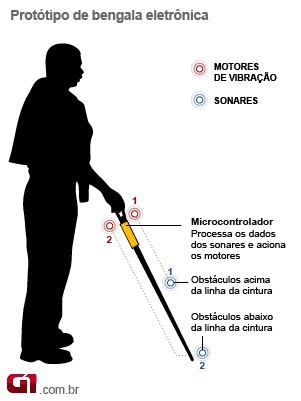
\includegraphics[width=0.4 \textwidth]{Figuras/bengala2.jpg}
  \\
  Disponível em: \url{https://www.deficienteciente.com.br/brasileiro-cria-bengala-eletronica-de-baixo-custo-para-deficientes-visuais.html} (Acessado em 01/04/2025)
  \label{fg-bengala}
\end{figure}
% --- FIM Figura

% --- Figura
\begin{figure}[htbp]
  \centering
  \caption{Sinalização por vibração}
  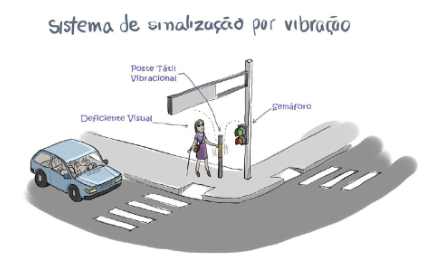
\includegraphics[width=0.6 \textwidth]{Figuras/sinal-vibra.png}
  \\
  Disponível em: \url{https://www.passeidireto.com/arquivo/79514730/deficiente-visual-e-o-transito-final} (Acessado em 01/04/2025)
  \label{fg-sinal}
\end{figure}
% --- Figura

% --- INÍCIO Figura
\begin{figure}[htbp]
  \centering
  \caption{Caneta falante}
  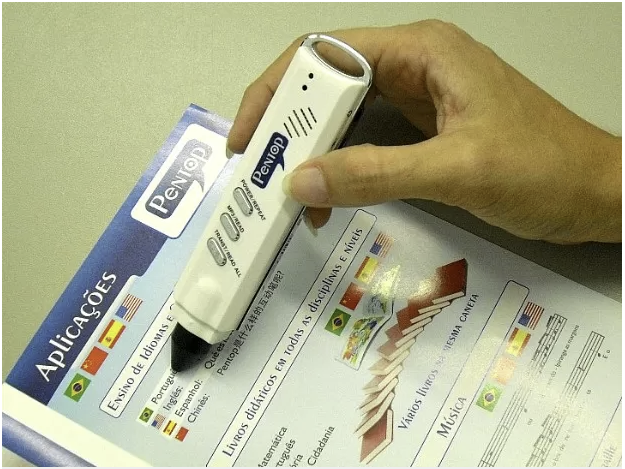
\includegraphics[width=0.8 \textwidth]{Figuras/caneta-fala.png}
  \\
  Disponível em: \url{https://g1.globo.com/am/amazonas/noticia/2012/09/caneta-que-fala-valor-do-dinheiro-para-deficientes-visuais-e-produzida-no-am.html} (Acessado em 01/04/2025)
  \label{fg-caneta}
\end{figure}
% --- FIM Figura

A visão computacional é um ramo da inteligência artificial que busca simular a capacidade humana de interpretar o ambiente por meio de imagens e vídeos. No campo da acessibilidade, ela tem sido empregada para desenvolver sistemas que reconhecem objetos, textos, rostos e sinais, oferecendo suporte para a orientação e interação de pessoas com deficiência visual com o mundo físico. Combinada a outros recursos, como sensores e \textit{feedback} auditivo, a visão computacional permite criar experiências assistivas mais ricas e contextualmente informadas \cite{Goodrich2020}.

Dentre as aplicações mais promissoras da visão computacional na assistência a pessoas cegas ou com baixa visão estão os sistemas de navegação autônoma em ambientes urbanos, o reconhecimento de sinais e placas, e a identificação de objetos em tempo real. Projetos como o Seeing AI, apresentado na Figura \ref{fg-seeing-ai}, da Microsoft, ou o OrCam MyEye, demonstram como dispositivos portáteis podem traduzir elementos visuais em áudio, promovendo independência funcional \cite{Li2021}. Embora esses sistemas tenham alcançado certo grau de sofisticação, ainda enfrentam limitações em ambientes muito específicos ou desorganizados, como é o caso de muitos campi universitários brasileiros.

% --- INÍCIO Figura
\begin{figure}[htbp]
  \centering
  \caption{Seeing Ai, Microsoft}
  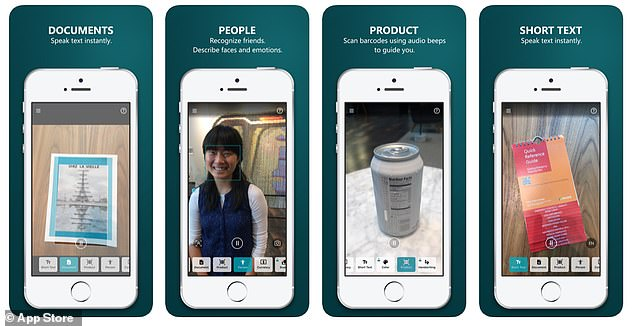
\includegraphics[width=0.8 \textwidth]{Figuras/seeing-ai.jpg}
  \\
  Disponível em: \url{https://ixd.prattsi.org/2024/09/assistive-technology-microsoft-seeing-ai/} (Acessado em 01/04/2025)
  \label{fg-seeing-ai}
\end{figure}
% --- FIM Figura

Apesar dos avanços, a maior parte dos sistemas comerciais apresenta limitações de contexto e adaptabilidade. Estudos como o de \citeonline{Martins2022} indicam que soluções importadas muitas vezes não se ajustam à realidade arquitetônica e cultural brasileira, seja por dificuldades na segmentação semântica de ambientes abertos, seja por falhas na detecção de objetos urbanos comuns no Brasil, como pontos de ônibus não padronizados ou faixas de pedestres pouco visíveis. Isso reforça a importância do desenvolvimento de sistemas contextualmente situados, com bases de dados e treinos locais, como proposto neste trabalho.

Uma característica central das tecnologias assistivas baseadas em visão computacional é o modo como os dados visuais são traduzidos em informação acessível. O \textit{feedback} auditivo é uma das interfaces mais eficazes para usuários com deficiência visual, pois permite a interpretação imediata de informações ambientais sem a necessidade de leitura tátil ou intervenção manual. Segundo \citeonline{Nguyen2020-feedback_strategies}, o uso de sinais auditivos diretos e contextuais reduz o tempo de resposta do usuário e aumenta sua percepção de controle sobre o ambiente, especialmente quando integrado com reconhecimento de objetos em vídeo.

Portanto, a aplicação da visão computacional com suporte de inteligência artificial em contextos assistivos não só é viável, como desejável do ponto de vista técnico e social. O uso de algoritmos robustos como o YOLO versão 11 (YOLOv11), que oferecem detecção em alta velocidade e com alta precisão, representa um avanço relevante frente aos métodos mais tradicionais. Como apontam \citeonline{redmon2018}, modelos da família YOLO são especialmente indicados para aplicações em tempo real e ambientes não controlados, características que se alinham perfeitamente à proposta deste trabalho no campus universitário.

\section{\textbf{Detecção de Objetos com Inteligência Artificial: O Algoritmo YOLOv11}}

Neste capítulo, são apresentados os fundamentos técnicos que sustentam o desenvolvimento da ferramenta proposta neste trabalho, com ênfase em visão computacional, aprendizado profundo e detecção de objetos com o algoritmo YOLOv11.

\subsection{\textbf{Fundamentos de Visão Computacional e Aprendizado Profundo}}

A visão computacional é um campo interdisciplinar que visa permitir que computadores interpretem e compreendam imagens e vídeos, simulando a capacidade perceptiva dos seres humanos, como mostrado na Figura \ref{fg-visao-computacional}. Essa área envolve diversas etapas, como a aquisição de imagens, o processamento digital, a análise e a interpretação de informações visuais. Ao longo das últimas décadas, avanços significativos em algoritmos, aumento de poder computacional e disponibilidade de grandes volumes de dados tornaram essa disciplina uma base essencial para soluções modernas em inteligência artificial  \cite{szeliski2022}.

% --- INÍCIO Figura
\begin{figure}[htbp]
  \centering
  \caption{Visão computacional - similaridade com percepção humana}
  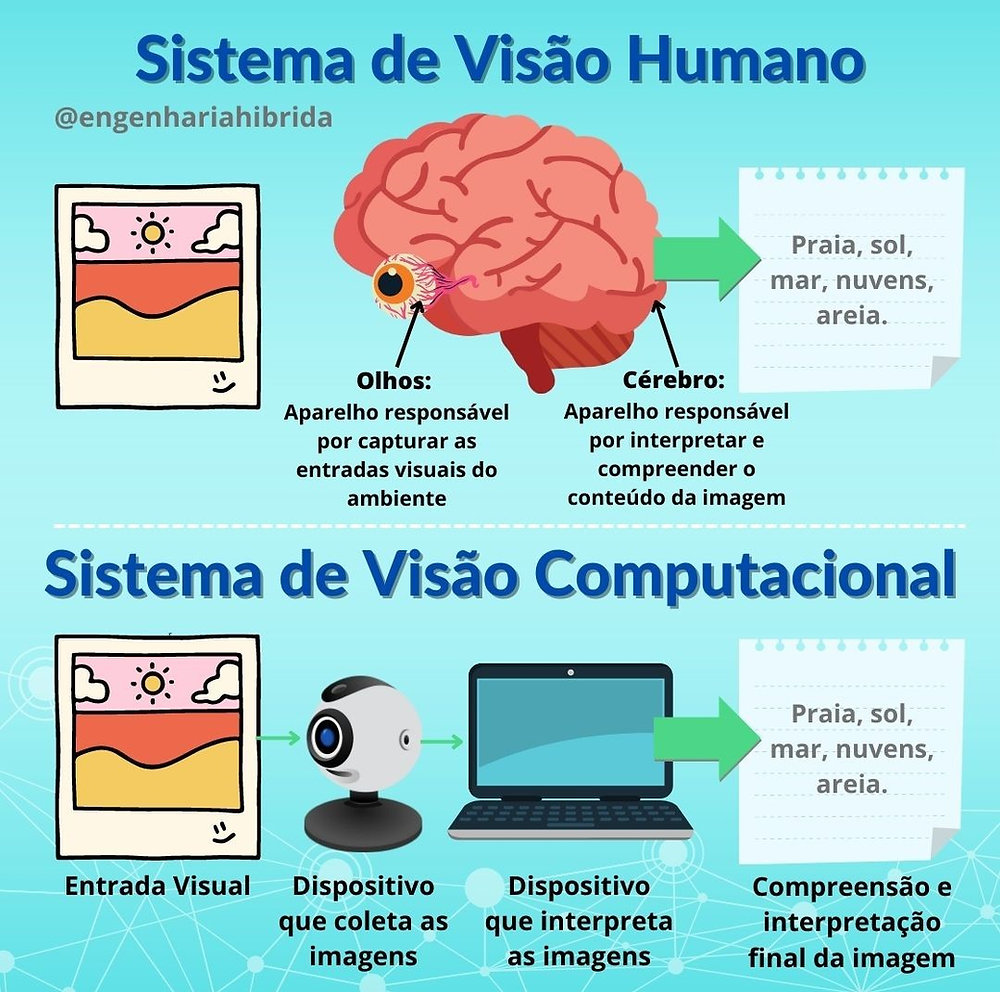
\includegraphics[width=0.8 \textwidth]{Figuras/visao-computacional.jpg}
  \\
  Disponível em: \url{https://www.engenhariahibrida.com.br/post/visao-computacional-como-funciona} (Acessado em 01/04/2025)
  \label{fg-visao-computacional}
\end{figure}
% --- FIM Figura

A aplicação da visão computacional se estende a diversas áreas, como medicina (diagnóstico por imagem), indústria (inspeção de qualidade), segurança (reconhecimento facial), transportes (veículos autônomos) e, mais recentemente, acessibilidade. Em contextos assistivos, sua aplicação visa melhorar a interação de pessoas com deficiência visual com o ambiente, oferecendo soluções de detecção e descrição auditiva de objetos e espaços \cite{goodfellow2016}.

A transformação mais significativa da visão computacional ocorreu com a introdução do aprendizado profundo, especialmente com as redes neurais convolucionais (CNNs). Essas redes se tornaram fundamentais para a análise de dados visuais, pois conseguem extrair características complexas das imagens de forma autônoma, sem necessidade de engenharia manual de atributos \cite{gu2018}.

Com a disseminação de ferramentas como TensorFlow, Keras e PyTorch, o desenvolvimento de aplicações de visão computacional com aprendizado profundo foi amplamente democratizado. Essas bibliotecas de utilização livre (\textit{open source}) permitem que pesquisadores e desenvolvedores criem modelos personalizados com maior facilidade, acelerando o processo de prototipagem e implantação \cite{hassaballah2020}.

Por fim, o avanço do \textit{hardware}, especialmente unidades de processamento gráfico (GPUs) e as unidades de processamento de tensor (TPUs), e a popularização de dispositivos móveis com capacidade de processamento elevado ampliaram ainda mais o campo de aplicação da visão computacional. Atualmente, sistemas inteligentes com reconhecimento de imagem podem ser executados em \textit{smartphones}, possibilitando aplicações portáteis e acessíveis, como é o caso do presente trabalho voltado para usuários com deficiência visual \cite{geron2022}.

\subsection{\textbf{Conceitos Básicos de Aprendizado Profundo}}

O aprendizado profundo é uma subárea do aprendizado de máquina que utiliza redes neurais artificiais com várias camadas para aprender representações hierárquicas dos dados. Essas redes são capazes de identificar padrões complexos por meio de sucessivas transformações não lineares dos dados de entrada, aproximando-se do comportamento de redes neurais biológicas \cite{goodfellow2016}).

Um dos principais diferenciais do aprendizado profundo é a sua capacidade de realizar a extração automática de características. Isso significa que, ao contrário de técnicas mais tradicionais, não há necessidade de que especialistas definam previamente os atributos que serão analisados: a própria rede aprende essas representações a partir dos dados \cite{Agarwal2021-deeplearning}.

A estrutura dessas redes, mostrada na Figura \ref{fg0}, inclui uma camada de entrada, múltiplas camadas ocultas e uma camada de saída. Cada camada realiza cálculos com base nas saídas das camadas anteriores, e as conexões entre os neurônios são ponderadas por valores ajustáveis durante o treinamento. Funções de ativação como a unidade linear retificada (ReLU) são essenciais para introduzir não linearidades no modelo, permitindo a representação de relações complexas \cite{gu2018}.

% --- Figura
\begin{figure}[htbp]
  \centering
  \caption{Estrutura de uma rede neural profunda}
  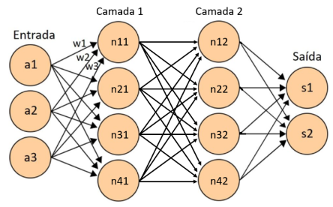
\includegraphics[width=0.6\textwidth]{Figuras/Est-rede-neural-profunda.png}
  \\
  Disponível em: \url{https://didatica.tech/introducao-a-redes-neurais-e-deep-learning/} (Acessado em 01/04/2025)
  \label{fg0}
\end{figure}
% --- Figura

\subsection{\textbf{Redes Neurais Convolucionais para Reconhecimento de Objetos}}
As CNNs foram projetadas especificamente para lidar com imagens. Inspiradas na organização do córtex visual dos mamíferos, essas redes exploram relações espaciais locais por meio do uso de filtros convolucionais, que varrem a imagem identificando padrões específicos em diferentes regiões \cite{lecun2015}.

Uma CNN, como mostrado na Figura \ref{fg-cnn}, é composta por várias camadas: convolucionais, de \textit{pooling} e totalmente conectadas. As camadas convolucionais aplicam filtros que produzem mapas de ativação, nos quais são realçadas características como bordas ou formas. As camadas de \textit{pooling} têm a função de reduzir a resolução espacial desses mapas, diminuindo a complexidade computacional e ajudando a evitar o sobreajuste \cite{gu2018}.

% --- Figura
\begin{figure}[htbp]
  \centering
  \caption{Estrutura de uma rede neural profunda}
  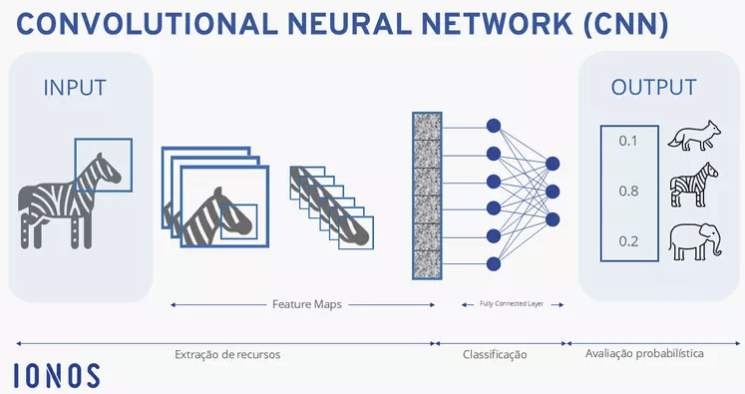
\includegraphics[width=0.8\textwidth]{Figuras/cnn.png}
  \\
  Disponível em: \url{https://www.ionos.com/pt-br/digitalguide/sites-de-internet/desenvolvimento-web/convolutional-neural-network/} (Acessado em 01/04/2025)
  \label{fg-cnn}
\end{figure}
% --- Figura

Um marco importante foi a criação da AlexNet em 2012, que venceu a competição ImageNet, demonstrando o potencial das CNNs em tarefas de larga escala \cite{krizhevsky2012}. Desde então, arquiteturas como VGG, GoogLeNet e ResNet ampliaram a profundidade e a eficiência das redes, contribuindo para a evolução da detecção de objetos.

A Figura \ref{fg1} detalha a arquitetura de AlexNet, uma rede neural convolucional que revolucionou a visão computacional ao vencer a competição ImageNet em 2012.

% --- Figura
\begin{figure}[htbp]
  \centering
  \caption{Arquitetura do AlexNet}
  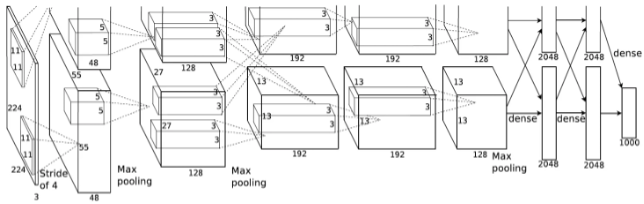
\includegraphics[width=1.0\textwidth]{Figuras/arquitetura-alexnet.png}
  \\
  Disponível em: \url{https://jefferson023.medium.com/alexnet-para-classifica%C3%A7%C3%A3o-de-imagens-d86c482a44b3} \\(Acessado em 01/04/2025)
  \label{fg1}
\end{figure}
% --- Figura

A eficiência computacional das CNNs permite que esses modelos sejam aplicados em tempo real ou quase tempo real, o que é essencial para sistemas assistivos com resposta imediata ao usuário \cite{bochkovskiy2020}.

\subsection{\textbf{Evolução e Funcionamento do Algoritmo YOLO}}

O algoritmo YOLO revolucionou a detecção de objetos ao propor uma abordagem unificada e extremamente rápida. Em vez de seguir o paradigma tradicional, que separava a tarefa em etapas como geração de propostas de região e posterior classificação, o YOLO trata toda a detecção como um problema de regressão direta, em que uma única rede neural realiza todas as previsões simultaneamente \cite{redmon2016}.

A imagem de entrada é dividida em uma grade, e cada célula dessa grade é responsável por prever várias caixas delimitadoras e suas respectivas probabilidades de classe. Essa abordagem permite que a detecção seja extremamente rápida, o que é essencial para aplicações em tempo real \cite{bochkovskiy2020}.

Como ilustrado na Figura \ref{fg2}, o algoritmo YOLO é capaz de realizar a detecção de objetos em tempo real, identificando múltiplos objetos em uma única imagem e delineando-os com \textit{bounding boxes}.

% --- Figura
\begin{figure}[htbp]
  \centering
  \caption{Detecção de objetos em tempo real com o YOLO}
  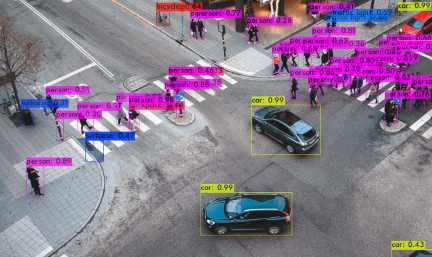
\includegraphics[width=1\textwidth]{Figuras/detec-yolo.png}
  \\
  Disponível em: \url{https://iaexpert.academy/2020/10/13/deteccao-de-objetos-com-yolo-uma-abordagem-moderna/?doing_wp_cron=1719375630.4834909439086914062500 } \\(Acessado em 01/04/2025)
  \label{fg2}
\end{figure}
% --- Figura

As versões subsequentes do YOLO, v3, v4, v5 até a v12, introduziram diversas melhorias, incluindo redes mais profundas, camadas residuais, normalização por lotes e previsão em múltiplas escalas \cite{bochkovskiy2020}.

O YOLOv11, desenvolvido pela Ultralytics, conta com uma infraestrutura moderna baseada em PyTorch, suporte nativo a exportação para ONNX e TensorRT, e integração com vídeos em tempo real, o que o torna altamente eficiente para aplicações práticas \cite{Ultralytics2024}.

\subsection{\textbf{Aplicação do YOLO em Tecnologias Assistivas}}

A detecção de objetos com o algoritmo tem sido amplamente explorada em projetos de tecnologias assistivas voltadas para pessoas com deficiência visual. A capacidade do algoritmo de realizar detecções em tempo real com alta precisão o torna ideal para aplicações que exigem respostas imediatas, como é o caso de sistemas de orientação pessoal e navegação urbana \cite{redmon2016}.

Diversos estudos têm utilizado o YOLO para construir sistemas portáteis que auxiliam deficientes visuais a identificar objetos e interagir com o ambiente. Por exemplo, \citeonline{Nguyen2020-smart_glasses} desenvolveram um sistema baseado em YOLOv3 embarcado em óculos inteligentes que detecta sinais de trânsito e envia mensagens de voz ao usuário. Outros projetos, como o de \citeonline{Khan2021}, usaram o YOLOv4 para detectar degraus, portas e semáforos, auxiliando na mobilidade autônoma em espaços urbanos.

A robustez do YOLO para detectar objetos diversos em diferentes condições ambientais é uma de suas principais vantagens em cenários assistivos. Isso permite que o algoritmo seja aplicado em ambientes dinâmicos e pouco padronizados, como é o caso de ruas, praças e campi universitários. Além disso, sua compatibilidade com dispositivos embarcados facilita a construção de sistemas de baixo custo e alta portabilidade \cite{bochkovskiy2020}.

Apesar de suas qualidades, o uso do YOLO em aplicações assistivas também enfrenta desafios. Entre eles estão a detecção de objetos pequenos ou parcialmente ocultos e a variabilidade de iluminação nos ambientes reais. Estudos como o de \citeonline{Li2022} apontam que a acurácia do algoritmo pode ser comprometida em condições adversas, o que reforça a necessidade de adaptações e treinamento com dados contextualizados.

\section{\textbf{Construção de conjunto de dados personalizados}}

A construção de conjunto de dados (\textit{datasets}) personalizados é uma etapa fundamental no desenvolvimento de sistemas de visão computacional baseados em aprendizado profundo. Enquanto grandes bancos de dados públicos, como ImageNet, COCO e Open Images, são amplamente utilizados para treinamentos genéricos, aplicações específicas exigem conjuntos de dados adaptados ao contexto e aos objetivos do projeto \cite{Zhou2017}.

Em projetos voltados para acessibilidade, como sistemas de assistência para pessoas com deficiência visual, a construção de um \textit{dataset} personalizado permite que o modelo aprenda padrões visuais diretamente relacionados ao ambiente de uso. Isso é particularmente importante em ambientes urbanos ou universitários, nos quais a variação de elementos arquitetônicos, sinalização e objetos é significativa e muitas vezes fora do escopo dos \textit{datasets} públicos \cite{Khan2021}.

A construção de um \textit{dataset} personalizado segue algumas etapas essenciais: i. captura de imagens ou vídeos, ii. seleção e extração de \textit{frames}, iii. anotação das \textit{bounding boxes} e, iv. classificação dos objetos. Diversas ferramentas auxiliam nesse processo, como o LabelImg, VoTT e o Roboflow, que oferecem interfaces intuitivas para rotulagem e exportação em formatos compatíveis com os principais modelos de detecção \cite{Tzutalin2015}.

Outro aspecto crítico é a qualidade e diversidade dos dados. Para que um modelo generalize bem, o \textit{dataset} deve incluir variações de iluminação, perspectiva, escala e posicionamento dos objetos. Técnicas de \textit{data augmentation}, como rotação, inversão, ajuste de brilho e aplicação de ruído, são comumente empregadas para ampliar artificialmente o volume de exemplos sem comprometer a veracidade das informações \cite{Shorten2019}.

Por fim, é importante que o \textit{dataset} reflita não apenas a variedade de situações do mundo real, mas também os objetivos da aplicação. Em projetos assistivos, por exemplo, pode ser mais relevante rotular elementos como rampas, escadas, sinalização auditiva ou superfícies táteis, em vez de objetos comuns como carros ou pessoas. A adequação do \textit{dataset} ao contexto real de uso é o que garante a efetividade prática do modelo treinado.

\section{\textbf{Sinais Auditivos e \textit{Feedback} em Sistemas Assistivos}}

Os sinais auditivos são amplamente utilizados como mecanismo de \textit{feedback} em tecnologias assistivas voltadas para pessoas com deficiência visual. Por meio de sons, alertas ou mensagens de áudio, esses sistemas fornecem informações essenciais sobre o ambiente, promovendo maior autonomia e segurança aos usuários \cite{Milella2014}.

A principal vantagem do \textit{feedback} auditivo é a capacidade de transmitir informações de forma não visual, liberando o sentido da audição para suprir a falta de percepção visual. Estudos mostram que sinais auditivos bem projetados contribuem significativamente para a localização de objetos, orientação espacial e prevenção de acidentes \cite{Nguyen2020-feedback_strategies}.

Existem diferentes abordagens para a implementação de \textit{feedback} auditivo em sistemas assistivos. Algumas utilizam sons padronizados para indicar a presença de um objeto, enquanto outras se valem de mensagens de voz geradas dinamicamente. A escolha da abordagem depende do tipo de informação a ser transmitida, da urgência do alerta e do contexto de uso \cite{Spagnol2018}.

Um desafio importante é evitar a sobrecarga auditiva do usuário. Sistemas que emitem muitos sons ou mensagens em sequência podem causar distração ou confusão. Por isso, boas práticas envolvem a hierarquização dos alertas, uso de sons distintos e ajustes dinâmicos de volume com base no nível de ruído ambiente \cite{Akbar2022}.

Diversos dispositivos já exploram com sucesso o uso de \textit{feedback} auditivo, como o OrCam MyEye - mostrado na Figura \ref{fg-orcammyeye}, o projeto Microsoft Seeing AI e soluções embarcadas com Raspberry Pi. Esses exemplos demonstram a viabilidade e a eficácia do uso de sinais auditivos como ponte entre a interpretação visual automatizada e a comunicação com o usuário final.

% --- Figura
\begin{figure}[htbp]
  \centering
  \caption{OrCam MyEye}
  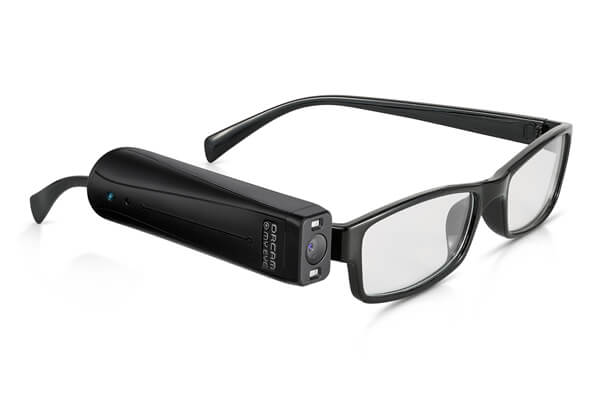
\includegraphics[width=0.8\textwidth]{Figuras/orcammyeye.jpg}
  \\
  Disponível em: \url{https://maisautonomia.com.br/produto/orcam-myeye-2-0/} \\(Acessado em 01/04/2025)
  \label{fg-orcammyeye}
\end{figure}
% --- Figura

\section{\textbf{Dispositivos e Plataformas para Tecnologias Assistivas Visuais}}

O desenvolvimento de dispositivos e plataformas tecnológicas voltados para pessoas com deficiência visual tem se expandido significativamente nos últimos anos, impulsionado pelos avanços em inteligência artificial, miniaturização de componentes e acessibilidade digital. Esses sistemas visam fornecer informações contextuais sobre o ambiente por meio de canais alternativos à visão, como a audição ou o tato, promovendo maior autonomia e inclusão \cite{Saeedi2021}.

Entre os dispositivos mais comuns estão os vestíveis do dia a dia, como óculos inteligentes e pulseiras sensoriais, que capturam dados do ambiente por meio de câmeras, sensores ultrassônicos, LiDAR e GPS, assim como fornecem \textit{feedback} em tempo real. Uma das iniciativas mais conhecidas é o OrCam MyEye, um pequeno dispositivo acoplado a óculos comuns, capaz de ler textos, reconhecer rostos e objetos, emitindo mensagens auditivas para o usuário \cite{OrCam2022}.

Outra plataforma amplamente reconhecida é o Microsoft Seeing AI, um aplicativo gratuito para \textit{smartphones} que utiliza visão computacional para descrever cenas, identificar produtos, reconhecer textos e até emoções faciais. O Seeing AI é um exemplo de solução acessível e eficaz, pois utiliza o \textit{hardware} já disponível em celulares modernos, dispensando a aquisição de dispositivos específicos \cite{Microsoft2023}.

Outras soluções têm apostado na integração de sensores múltiplos para oferecer navegação segura em tempo real. O projeto BLAID da Toyota, por exemplo, propõe um dispositivo vestível que combina visão computacional com sensores de profundidade para detectar obstáculos e orientar o deslocamento em ambientes internos, como corredores e escadas \cite{Toyota2018}.

Além dos dispositivos vestíveis e aplicativos móveis, plataformas embarcadas como Raspberry Pi e Arduino são comumente utilizadas em projetos de pesquisa e prototipagem rápida. Essas placas de baixo custo permitem a criação de sistemas personalizados, com câmeras e atuadores auditivos, sendo muito utilizadas em ambientes acadêmicos como parte de soluções educacionais acessíveis \cite{Pino2020}.

A escolha entre dispositivos dedicados e soluções baseadas em \textit{smartphones} depende de fatores como custo, portabilidade, facilidade de uso e escalabilidade. Aplicativos móveis são vantajosos pela ubiquidade dos celulares e atualização constante via \textit{software}, enquanto dispositivos dedicados, como óculos inteligentes, oferecem maior integração sensorial e desempenho específico \cite{Saeedi2021}.

Por fim, é importante destacar que a eficácia desses dispositivos não depende apenas de sua sofisticação tecnológica, mas também da sua usabilidade e adaptação ao contexto do usuário. Sistemas com interfaces intuitivas, comandos por voz e \textit{feedback} personalizado são os que tendem a gerar maior aceitação e impacto positivo na vida de pessoas com deficiência visual. A revisão das plataformas existentes contribui, portanto, para fundamentar as escolhas tecnológicas feitas no presente trabalho.

\section{\textbf{Avaliação da Efetividade em Tecnologias Assistivas}}
A avaliação da efetividade de tecnologias assistivas é uma etapa essencial para garantir que as soluções tecnológicas desenvolvidas realmente atendam às necessidades dos usuários com deficiência. Esse processo vai além da validação técnica e contempla aspectos como usabilidade, acessibilidade, satisfação do usuário, segurança e impacto na qualidade de vida \cite{Wentz2013}.

Um dos principais métodos para avaliação de sistemas assistivos é a aplicação de testes com usuários reais em ambientes controlados e em situações reais de uso. Esses testes permitem identificar barreiras de uso, falhas de comunicação entre sistema e usuário, e oportunidades de melhoria. O uso de entrevistas, questionários e observação direta são ferramentas valiosas nesse contexto \cite{Kintsch2002}.

Outra abordagem relevante é a aplicação de instrumentos padronizados de avaliação, como a escala de usabilidade do sistema, que fornece um índice quantitativo da usabilidade percebida pelo usuário. Esses instrumentos têm a vantagem de permitir a comparação entre diferentes tecnologias e protótipos, oferecendo uma base objetiva para tomada de decisão sobre aprimoramentos \cite{Brooke1996}.

A avaliação também deve considerar os princípios das diretrizes internacionais de acessibilidade digital mesmo quando o sistema não for estritamente digital. Esses princípios ajudam a garantir que as interfaces, alertas auditivos e formas de interação sejam compatíveis com diferentes perfis de usuários \cite{W3C2023}.

Estudos de caso com aplicação em campo são considerados uma das formas mais ricas de avaliação, pois permitem observar o impacto da tecnologia em situações reais e sob condições não controladas. Avaliações longitudinais, com acompanhamento ao longo do tempo, são especialmente valiosas para verificar adesão ao uso e impactos duradouros \cite{Batavia1990}.

Por fim, o envolvimento direto dos usuários com deficiência visual em todas as fases do desenvolvimento e da avaliação do sistema contribui para a construção de soluções centradas nas pessoas. Essa abordagem participativa tem sido promovida como uma boa prática no âmbito do design universal e da inclusão digital \cite{Story1998}.

\section{\textbf{Ética e Responsabilidade no Uso de Inteligência Artificial Assistiva}}

O uso de inteligência artificial (IA) em tecnologias assistivas levanta questões éticas relevantes que vão além da eficiência técnica. Ao lidar com dados sensíveis, como imagens do ambiente e comportamentos dos usuários, esses sistemas devem ser projetados considerando princípios como privacidade, segurança, transparência e não discriminação \cite{Floridi2018}.

A coleta e o processamento de imagens em tempo real, por exemplo, podem expor terceiros inadvertidamente, levantando preocupações sobre consentimento e anonimato. Em ambientes universitários ou urbanos, onde há tráfego constante de pessoas, é fundamental garantir que os dados captados não sejam armazenados indevidamente ou utilizados para outros fins sem autorização \cite{Jobin2019}.

Outro aspecto crítico é o viés algorítmico. Modelos de IA treinados com bases de dados pouco diversificadas podem apresentar desempenho inferior para determinados grupos, perpetuando desigualdades. Em tecnologias assistivas, isso pode significar falhas na detecção de objetos relevantes em contextos específicos, como escolas públicas, periferias ou comunidades rurais \cite{Buolamwini2018}.

A transparência também é uma exigência crescente. Usuários de sistemas assistivos têm direito a compreender como as decisões são tomadas, como os dados são processados e que garantias existem contra erros. Para isso, boas práticas incluem o fornecimento de informações acessíveis, documentação clara e possibilidade de auditoria \cite{Morley2020}.

Responsabilidade legal também é um ponto sensível: quem responde por falhas de um sistema assistivo automatizado? Fabricante, desenvolvedor, instituição usuária? A ausência de regulamentações específicas para IA em muitos países torna essencial a adoção de princípios de ética por design, ou seja, a incorporação de valores humanos e sociais desde o início do desenvolvimento \cite{Dignum2019}.

Esforços internacionais como o da Organização das Nações Unidas para a Educação, a Ciência e a Cultura (UNESCO) e da União Europeia têm buscado estabelecer diretrizes para o uso ético da IA. O Brasil também avança com a Estratégia Brasileira de Inteligência Artificial, que destaca a inclusão, a proteção de dados e os direitos humanos como pilares para o uso consciente dessas tecnologias \cite{MCTI2021}.

\section{\textbf{Considerações Finais}}

Diante desse cenário, este trabalho busca contribuir com a inclusão universitária por meio do desenvolvimento de uma ferramenta baseada em visão computacional, capaz de reconhecer elementos do ambiente físico da UFMG e fornecer \textit{feedback} auditivo em tempo real ao usuário com deficiência visual. A seguir, discute-se o panorama das tecnologias assistivas baseadas em visão computacional. 

Para que sistemas assistivos baseados em visão computacional sejam eficazes, é essencial que estejam sintonizados com o ambiente onde serão utilizados. A utilização de vídeos capturados diretamente no campus da UFMG e a construção de um \textit{dataset} com objetos de interesse locais, como faixas de pedestre, bancos e placas, permite uma adaptação do sistema às condições reais de uso. Essa abordagem é consistente com recomendações de estudos recentes, que destacam a importância da coleta de dados em contextos específicos para aumentar a precisão da detecção e a usabilidade final \cite{Borges2023}. 
\chapter{\textbf{METODOLOGIA}}
\section{\textbf{Levantamento Exploratório de Tecnologias Assistivas}}

Nesta etapa, é realizado um levantamento de soluções tecnológicas assistivas que utilizam visão computacional para auxiliar pessoas com deficiência visual. O foco é identificar abordagens técnicas recentes, algoritmos eficazes e boas práticas relevantes para aplicações de detecção de objetos em tempo real.

São analisados artigos científicos, repositórios públicos e demonstrações práticas de sistemas existentes. A comparação entre diferentes algoritmos, como SSD, Faster R-CNN e YOLO, revela que o YOLO se destaca pelo equilíbrio entre acurácia e velocidade, sendo adotado como base do presente projeto. Também é observada a ampla adoção de técnicas como \textit{transfer learning} e o uso de modelos pré-treinados para agilizar a adaptação a conjuntos de dados específicos.

Para confirmar a escolha, são testadas diferentes versões do YOLO (v8 a v11) sobre um mesmo vídeo gravado no campus da UFMG. As versões yolo8m, yolo9m, yolo10m e yolo11m são comparadas em termos de velocidade de inferência, precisão das caixas delimitadoras e estabilidade das detecções. O modelo yolo11m.pt apresenta o melhor desempenho e é selecionado para os próximos estágios do projeto.

Além da análise técnica, também é avaliada a viabilidade de implementação em ambientes externos e a clareza do feedback auditivo. A solução final é planejada com base em três objetos de interesse: bancos, faixas de pedestre e placas de ponto de ônibus, priorizando robustez, baixo custo computacional e utilidade prática no contexto do campus.

\section{\textbf{Ferramentas, Recursos e Ambiente de Desenvolvimento}}

O sistema é desenvolvido na linguagem Python 3.11.12, com execução em notebooks Jupyter no ambiente Google Colab. Essa plataforma oferece acesso gratuito a GPUs NVIDIA Tesla T4 com 15 \textit{Gigabytes} (GB) de \textit{video random-access memory} (VRAM), viabilizando o treinamento eficiente do modelo sem a necessidade de \textit{hardware} local. Os arquivos de vídeo, datasets e modelos treinados são armazenados no Google Drive, facilitando a integração e continuidade do projeto em diferentes dispositivos.

A principal biblioteca utilizada para detecção de objetos é a Ultralytics YOLOv11, escolhida por sua interface simplificada, suporte nativo a datasets customizados e bom desempenho em tarefas de tempo real. O modelo de base adotado é o yolo11m.pt, que apresenta equilíbrio entre velocidade e acurácia. A manipulação e visualização dos resultados ocorrem com a biblioteca OpenCV, responsável pela renderização das \textit{bounding boxes}, rótulos de classe, linhas divisórias na imagem e textos com valores de confiança.

A construção e anotação do dataset são realizadas na plataforma Roboflow, que permite \textit{upload} de imagens, rotulagem precisa, aplicação de técnicas de \textit{data augmentation} e exportação direta para o Colab via \textit{application programming interface} (API). A ferramenta também fornece relatórios visuais sobre a distribuição das classes e garante controle sobre a divisão entre treino e validação. Para a geração dos alertas sonoros, é usada a biblioteca gTTS, com sincronização de áudio e vídeo feita via MoviePy.

Outras bibliotecas complementares utilizadas incluem NumPy, para verificação de proximidade espacial e aplicação de filtros de debouncing, e logging, para o registro automatizado de eventos e erros durante a execução. Todas as ferramentas utilizadas são de código aberto e amplamente documentadas, promovendo a reprodutibilidade, portabilidade e acessibilidade do sistema.

A Figura \ref{fg-tecnologias-logos} mostra visualmente as principais tecnologias utilizadas neste trabalho.
% --- INÍCIO Figura
\begin{figure}[htbp]
  \centering
  \caption{Logos das principais tecnologias utilizadas neste trabalho}
  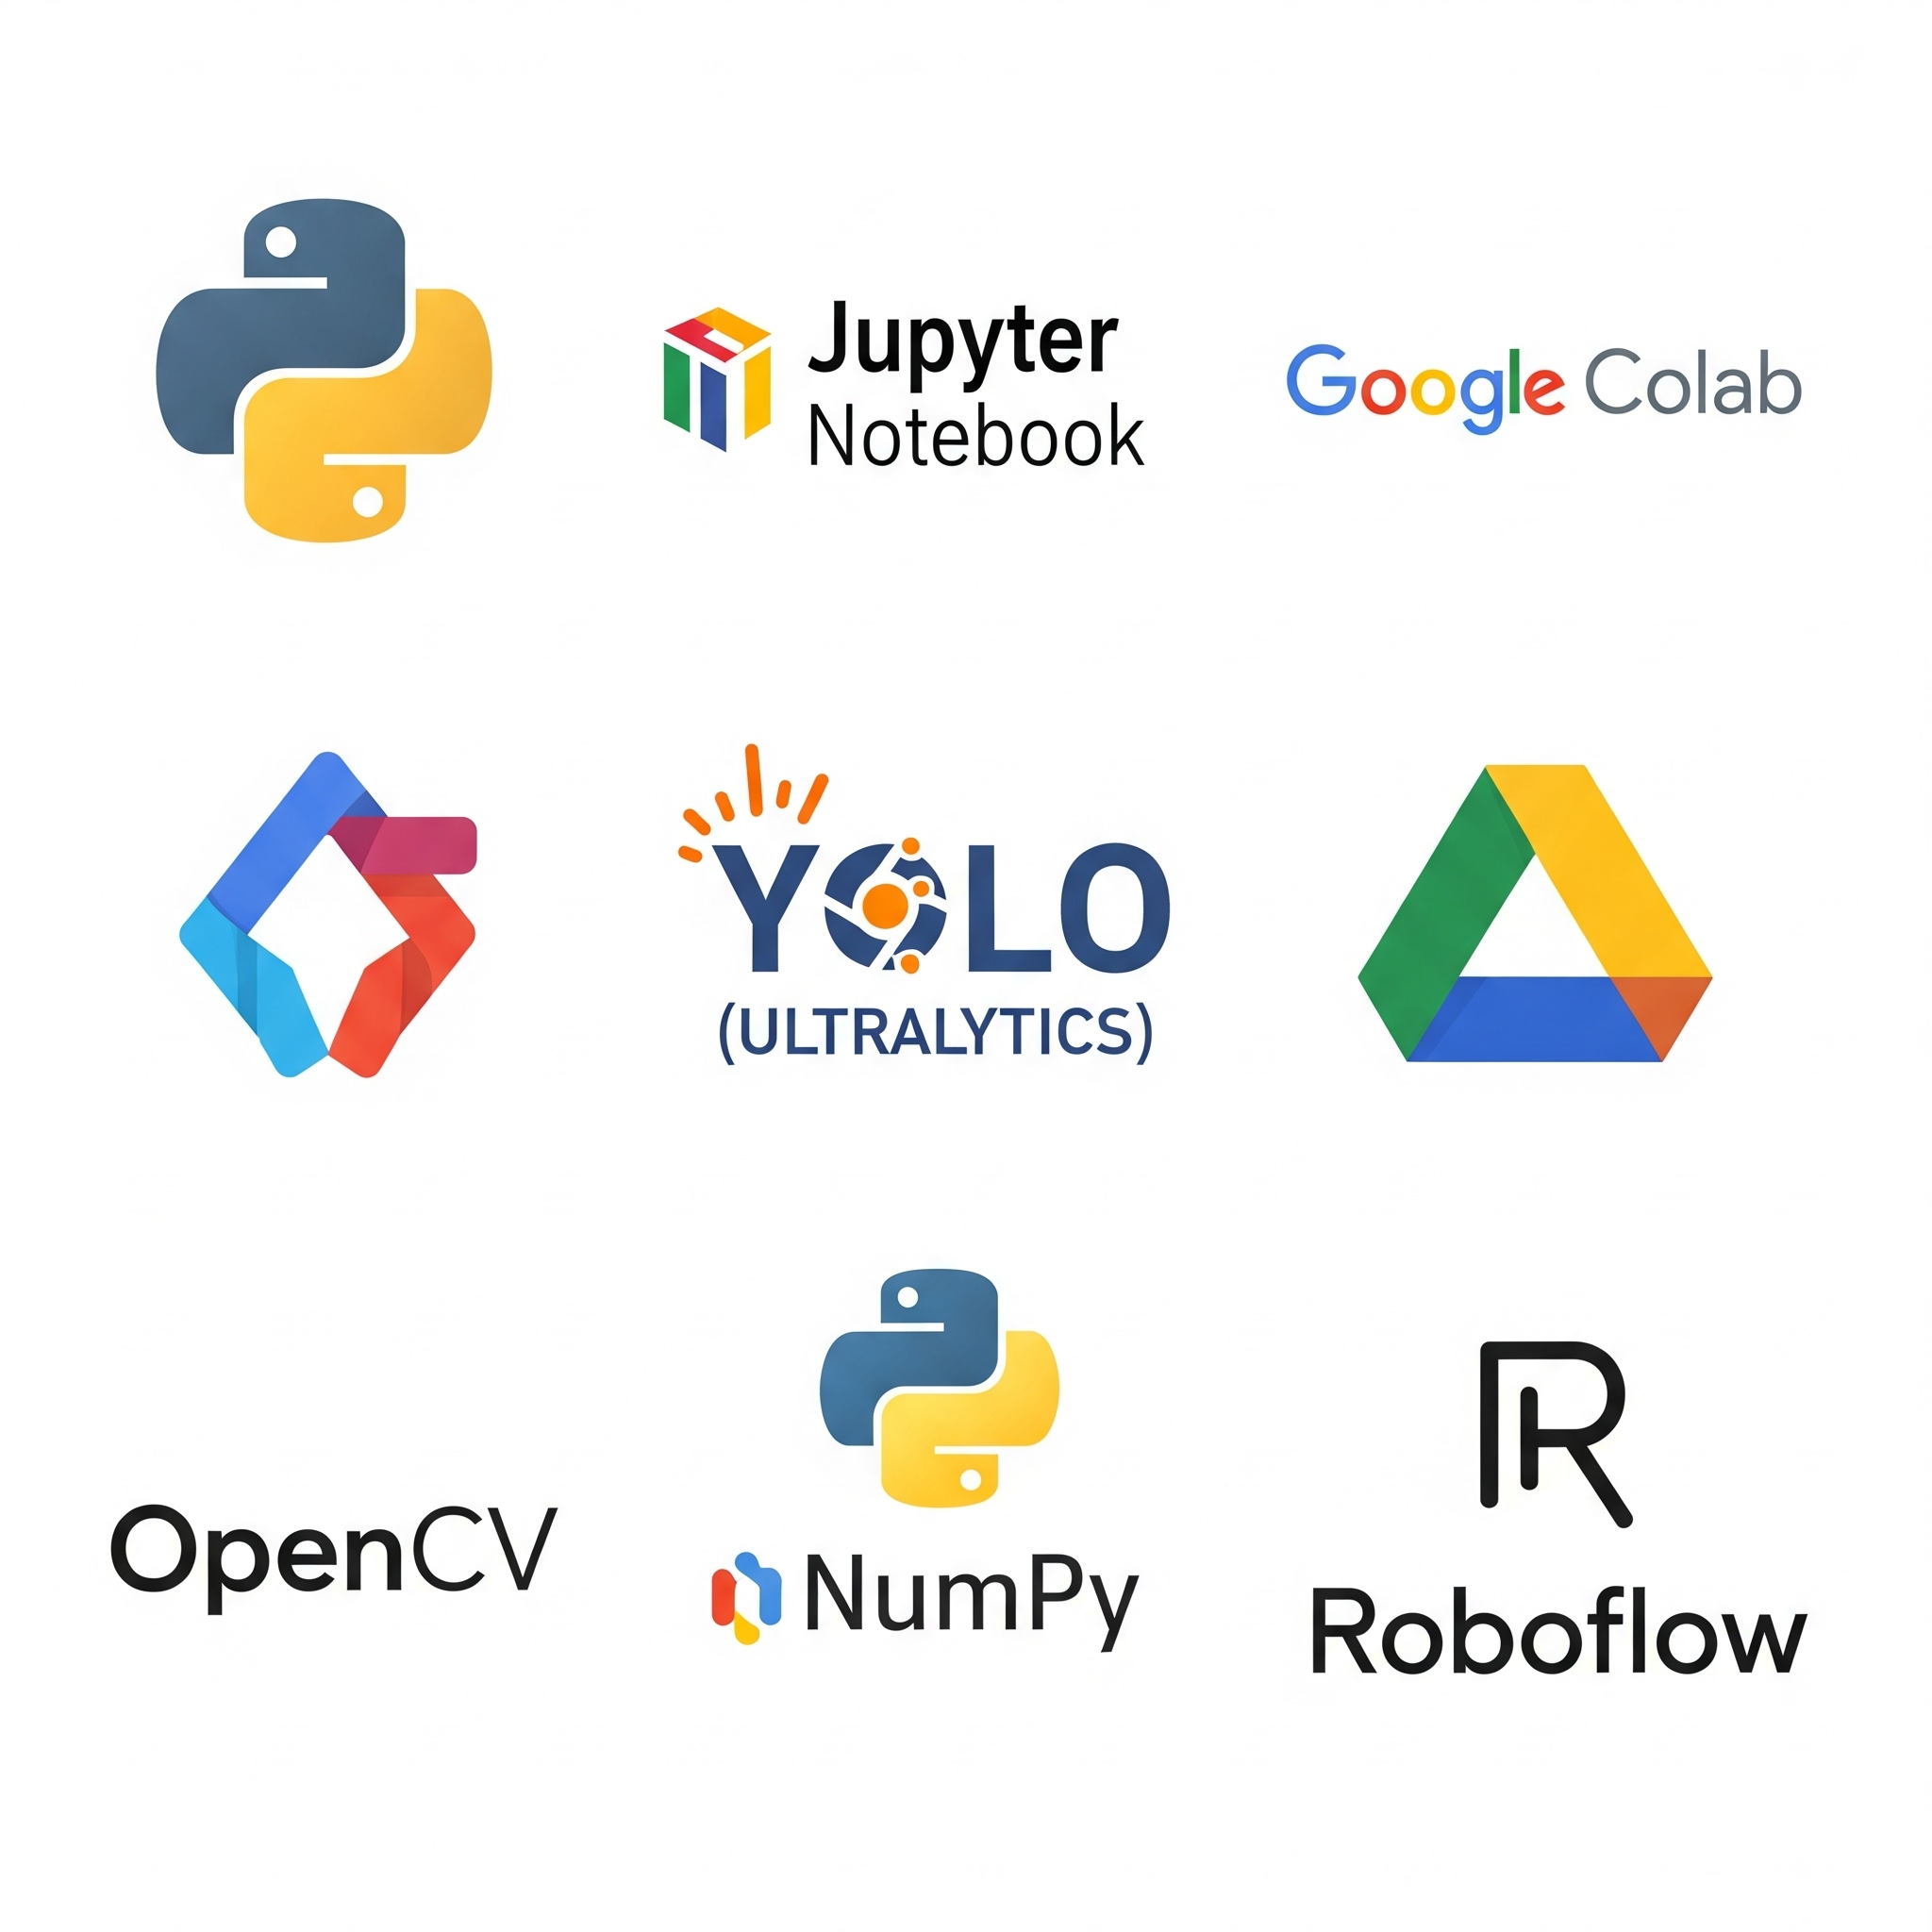
\includegraphics[width=0.6 \textwidth]{Figuras/tecnologias_logos.png}
  \\
  Fonte: Google Gemini.
  \label{fg-tecnologias-logos}
\end{figure}
% --- FIM Figura

\section{\textbf{Coleta de Dados Visuais no Ambiente-Alvo}}

A coleta de dados visuais é realizada no campus Pampulha da UFMG, ambiente escolhido por reunir circulação real de estudantes e variabilidade de cenários urbanos, como ruas internas, praças e paradas de ônibus. As gravações ocorrem em múltiplos dias e horários, abrangendo diferentes condições de luminosidade (manhã, tarde e noite) e de fluxo de pessoas, a fim de garantir diversidade nos dados. As Figuras \ref{fg-exe_grav_dia} e \ref{fg-exe_grav_noite} mostram exemplos diurnos e noturnos das fotos utilizadas.

% --- INÍCIO Figura
\begin{figure}[htbp]
  \centering
  \caption{Exemplo de foto diurna}
  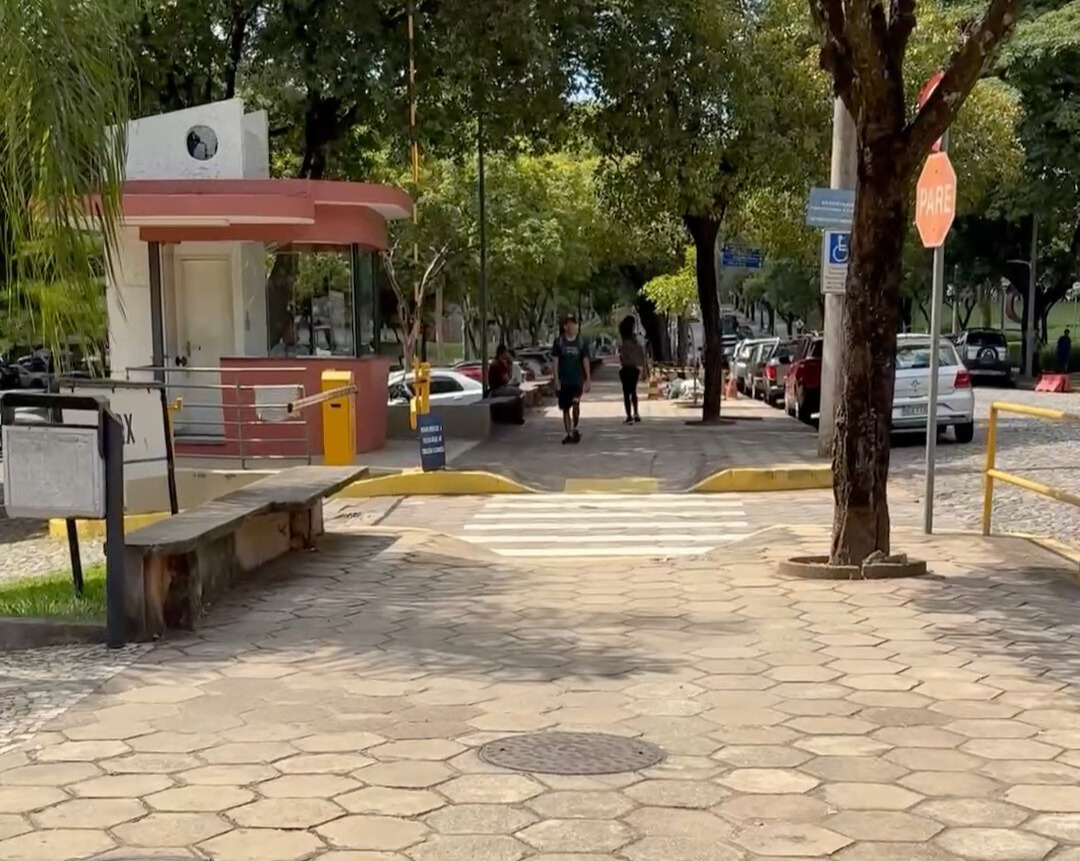
\includegraphics[width=0.8 \textwidth]{Figuras/exe_grav_dia - Editado.jpg}
  \\
  Fonte: Autoral.
  \label{fg-exe_grav_dia}
\end{figure}
% --- FIM Figura

% --- INÍCIO Figura
\begin{figure}[htbp]
  \centering
  \caption{Exemplo de foto noturna}
  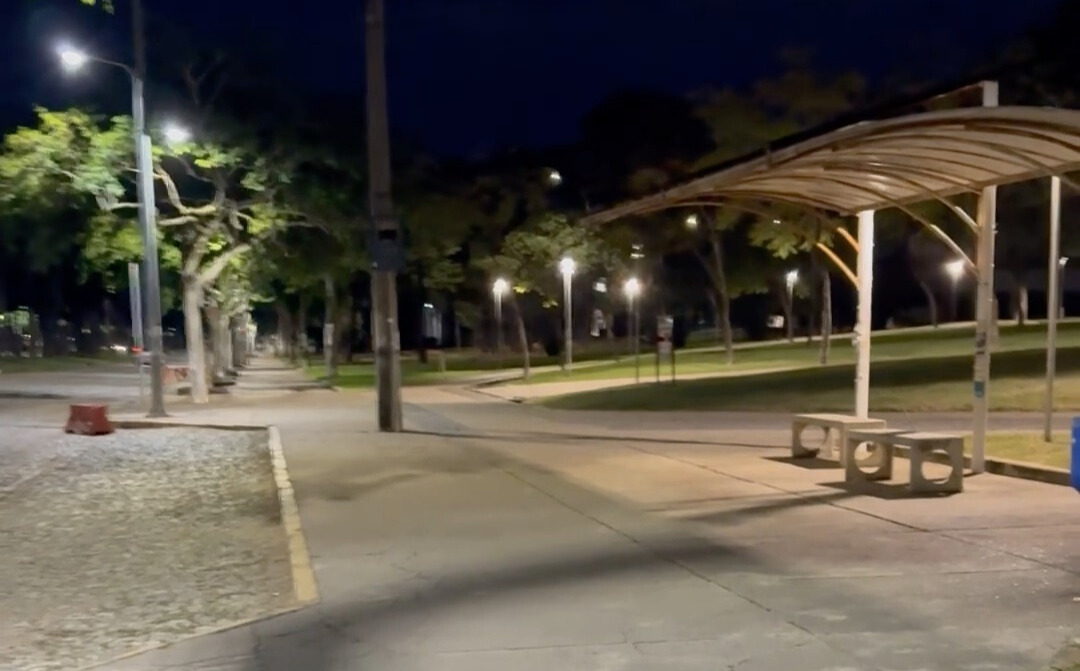
\includegraphics[width=0.8 \textwidth]{Figuras/exe_grav_noite - Editado.jpg}
  \\
  Fonte: Autoral.
  \label{fg-exe_grav_noite}
\end{figure}
% --- FIM Figura

Os vídeos são capturados com um smartphone posicionado na altura do peito, simulando a perspectiva de um usuário caminhando. Essa abordagem reproduz uma situação prática de uso em aplicações futuras. Todos os vídeos seguem configuração padronizada de resolução e taxa de quadros para manter consistência na captura.

Ao longo da coleta, são priorizados pontos do campus que contenham os três objetos de interesse: bancos, faixas de pedestre e placas de ponto de ônibus. A diversidade dos cenários permite treinar o modelo com diferentes formas, tamanhos e condições visuais dos objetos, incluindo situações com iluminação artificial, sombras acentuadas e obstruções parciais.

A extração de imagens dos vídeos é feita na plataforma Roboflow, resultando em aproximadamente 600 frames anotados. Cuidados éticos são tomados: evita-se focar em rostos ou informações pessoais, e os dados são usados exclusivamente para fins acadêmicos. Essa etapa assegura que o modelo seja treinado com dados realistas, aumentando sua robustez e aplicabilidade prática no mesmo ambiente onde será utilizado.

\section{\textbf{Preparação do \textit{Dataset} Personalizado}}

O dataset personalizado é construído com base em imagens extraídas dos vídeos gravados no campus Pampulha da UFMG. As três classes definidas para reconhecimento são: banco, faixa\_pedestre e placa\_onibus, escolhidas por sua relevância na navegação de pessoas com deficiência visual. Os frames são selecionados de forma a abranger diferentes horários do dia e níveis de ocupação do campus, garantindo diversidade nas condições de captura.

A anotação dos objetos é realizada manualmente na plataforma Roboflow, utilizando \textit{bounding boxes} para delimitar com precisão cada instância das classes de interesse. São anotadas mais de 600 imagens originais, com atenção à padronização dos nomes e ao formato das caixas, evitando inconsistências que possam prejudicar o aprendizado do modelo. As Figuras \ref{fg-ex_anot1}, \ref{fg-ex_anot2} e \ref{fg-ex_anot3} mostram exemplos de imagens anotadas no \textit{dataset} personalizado.

% --- INÍCIO Figura
\begin{figure}[htbp]
  \centering
  \caption{Exemplos de imagens com anotações realizadas}
  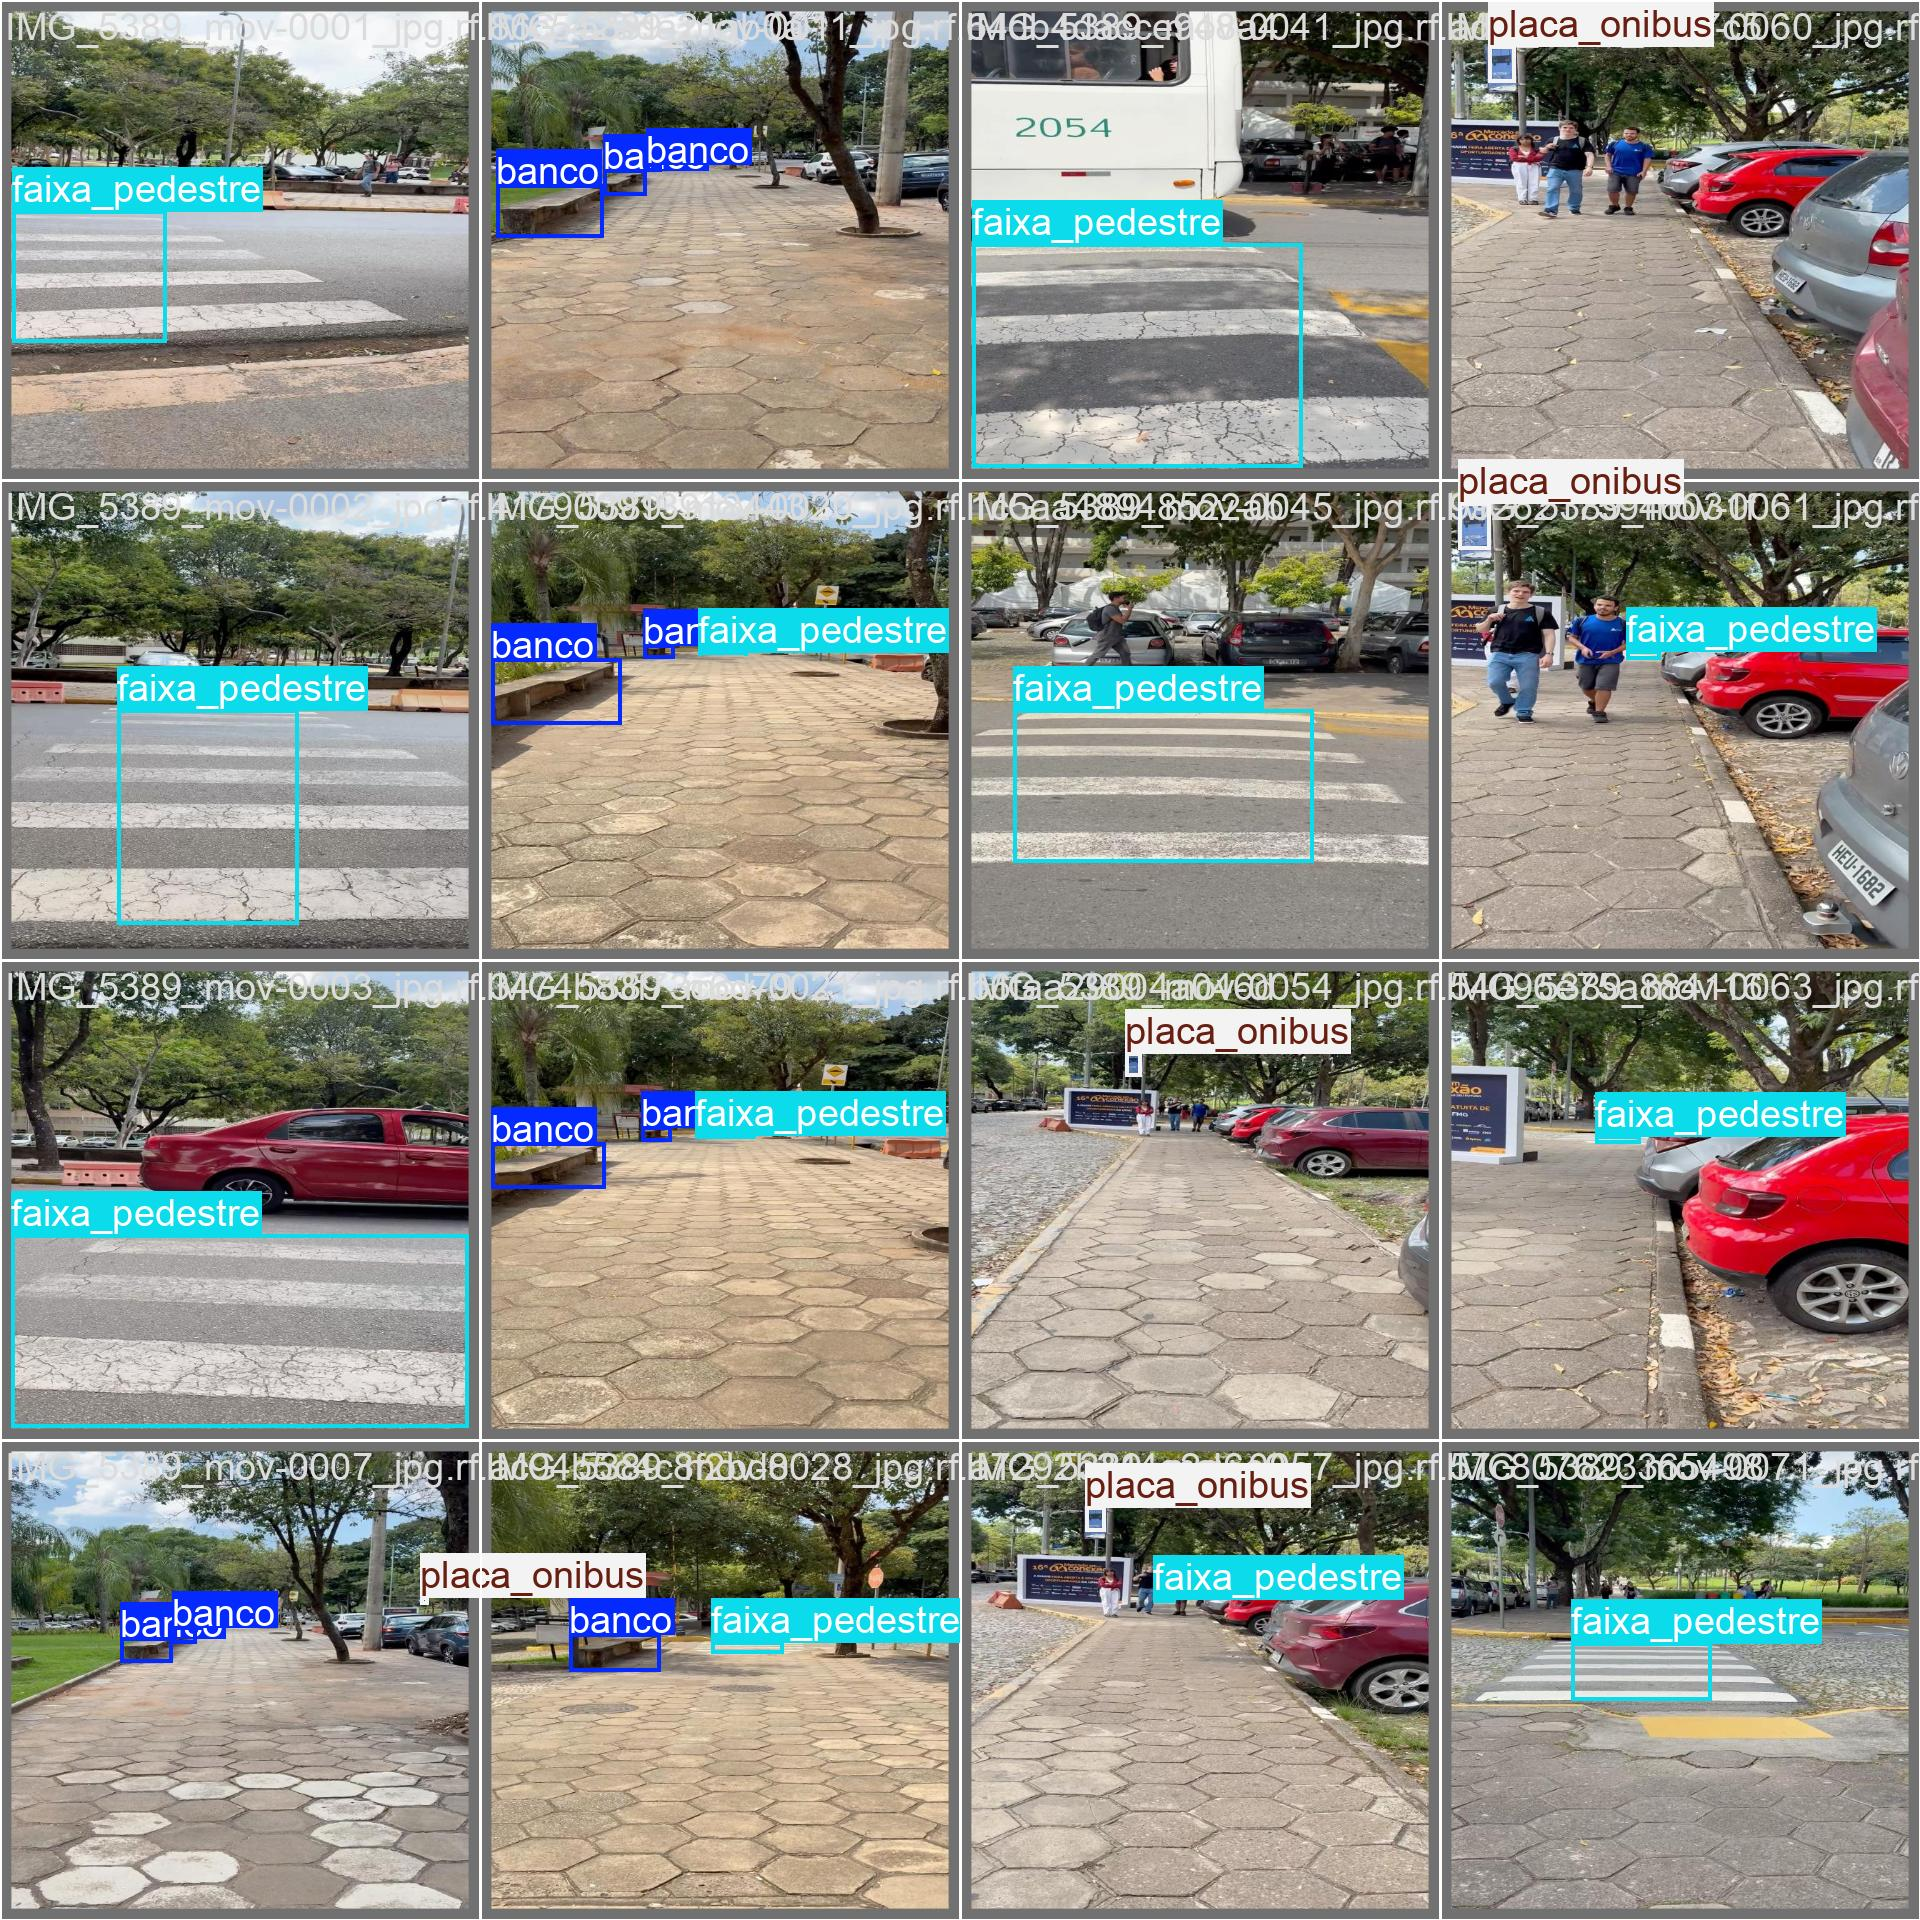
\includegraphics[width=1 \textwidth]{Figuras/val_batch0_labels.jpg}
  \\
  Fonte: Autoral.
  \label{fg-ex_anot1}
\end{figure}
% --- FIM Figura

% --- INÍCIO Figura
\begin{figure}[htbp]
  \centering
  \caption{Exemplos de imagens com anotações realizadas}
  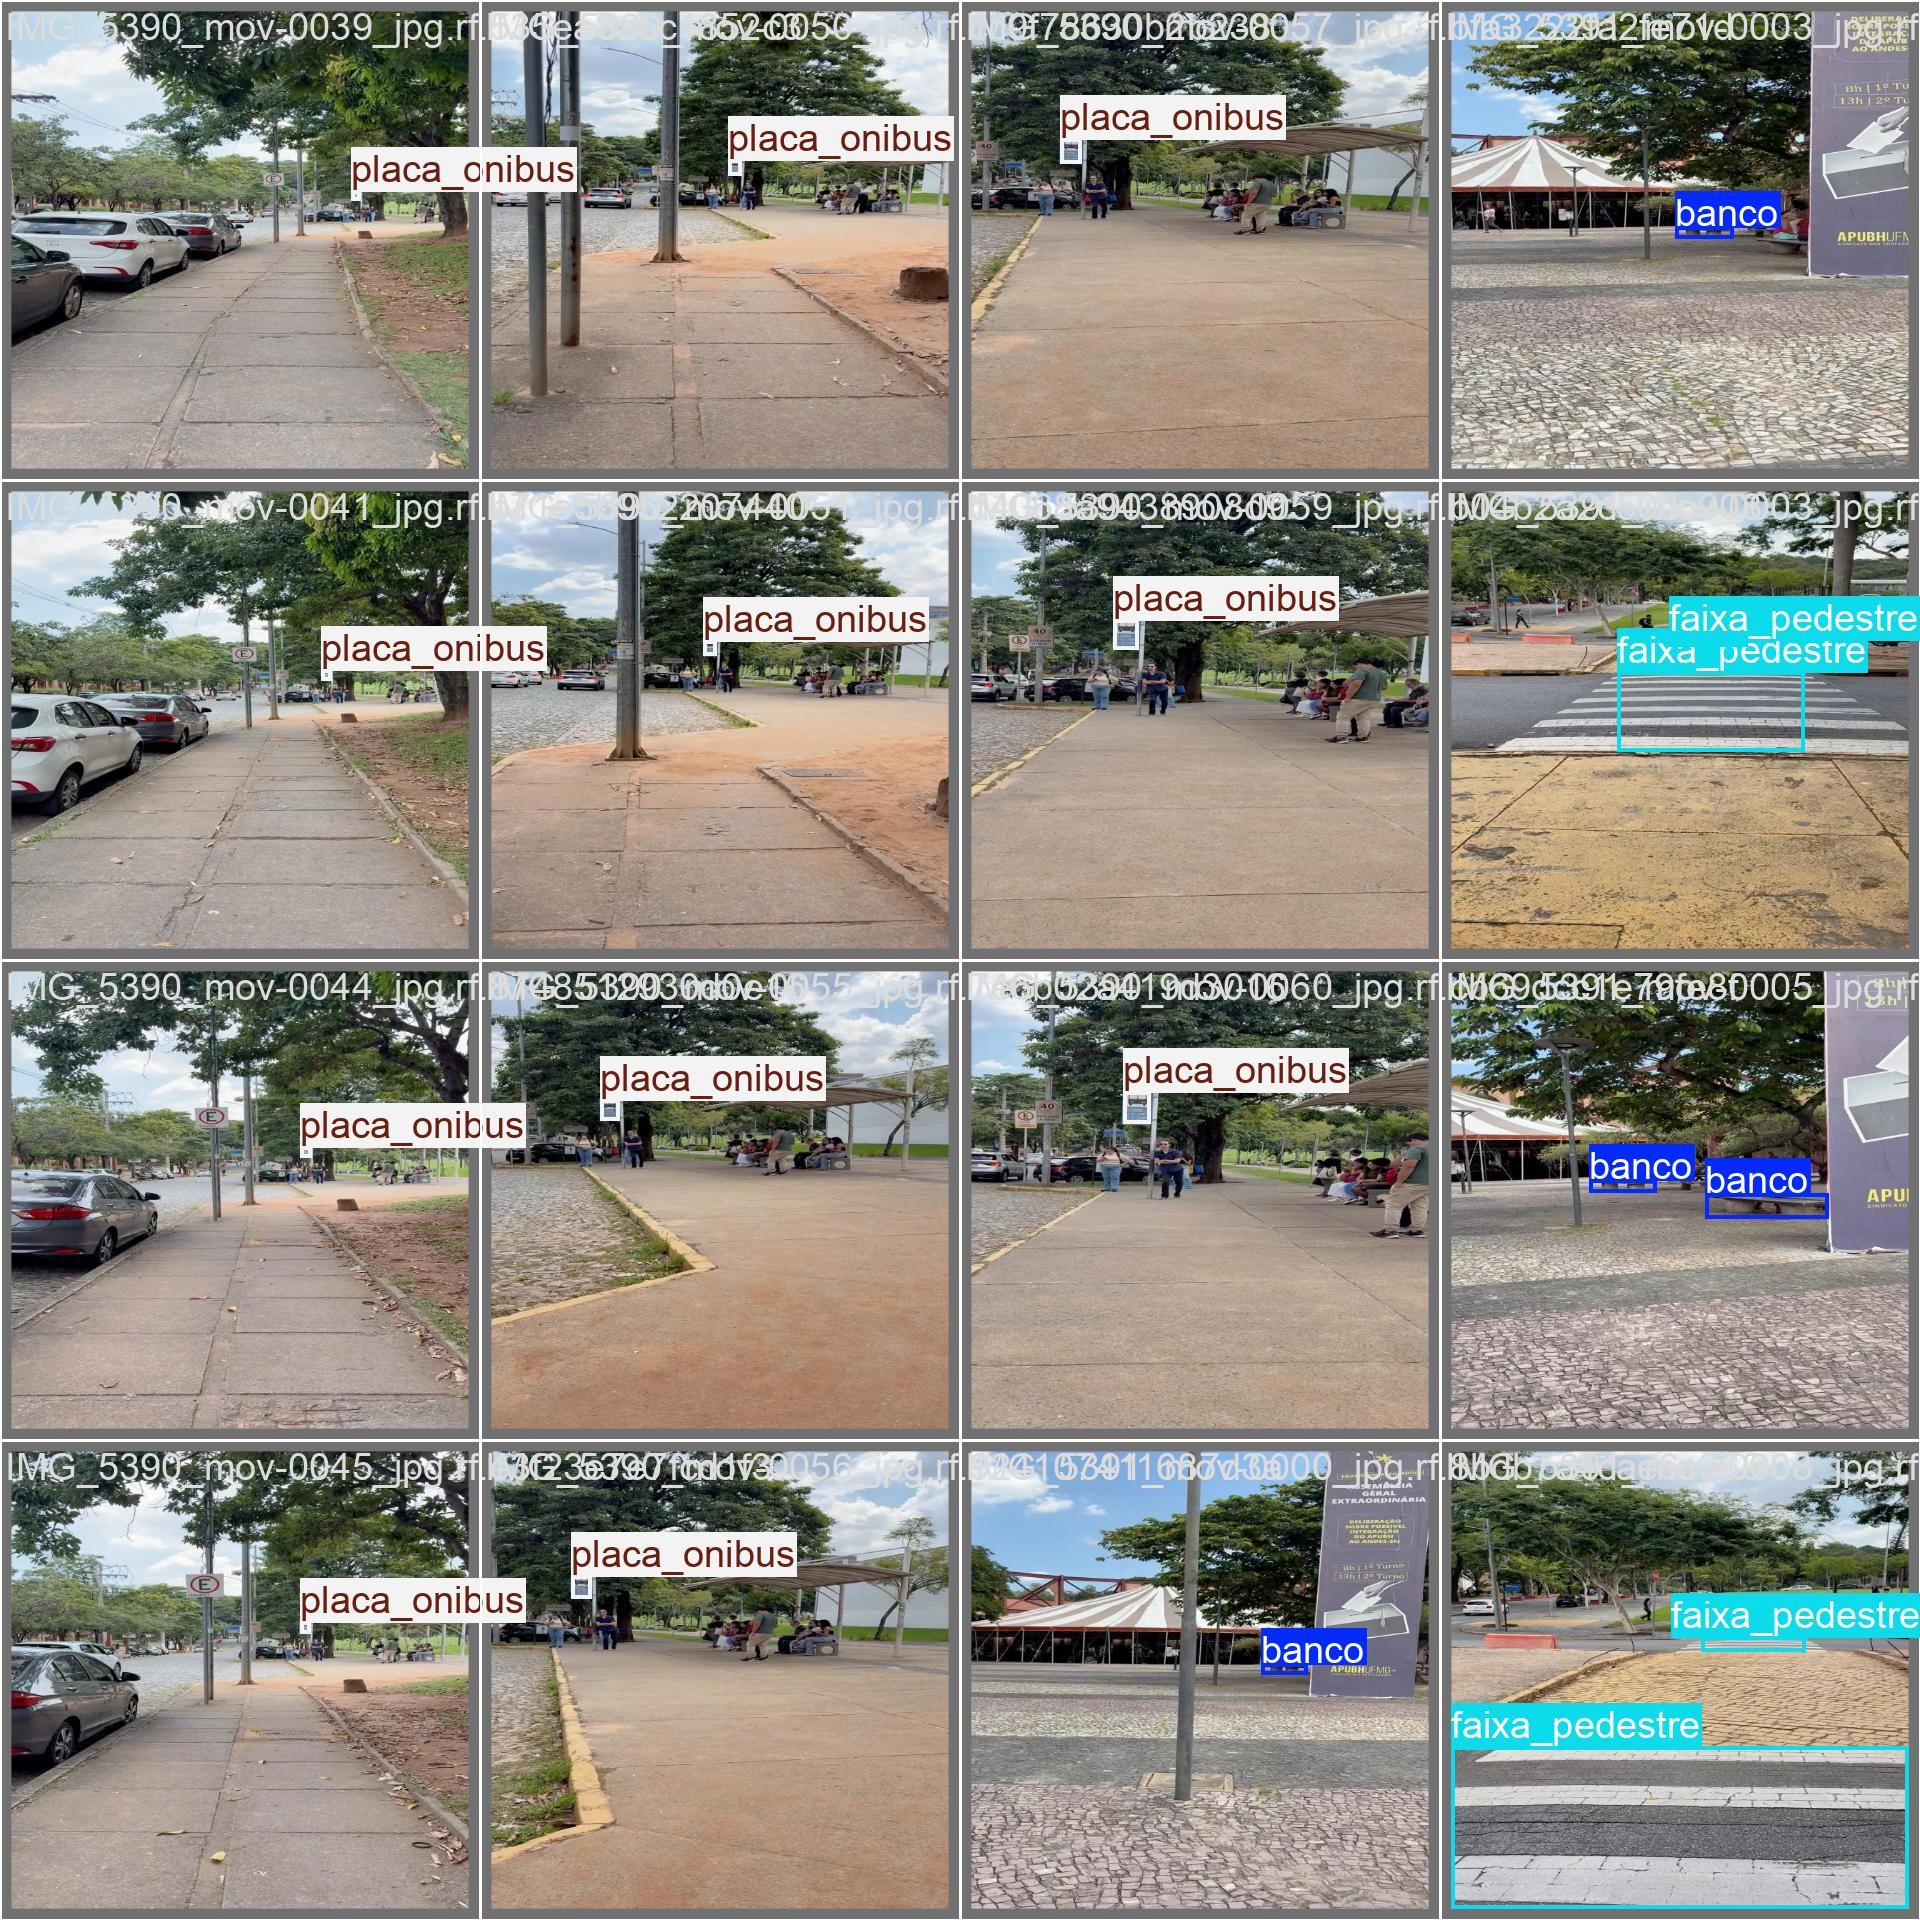
\includegraphics[width=1 \textwidth]{Figuras/val_batch1_labels.jpg}
  \\
  Fonte: Autoral.
  \label{fg-ex_anot2}
\end{figure}
% --- FIM Figura

% --- INÍCIO Figura
\begin{figure}[htbp]
  \centering
  \caption{Exemplos de imagens com anotações realizadas}
  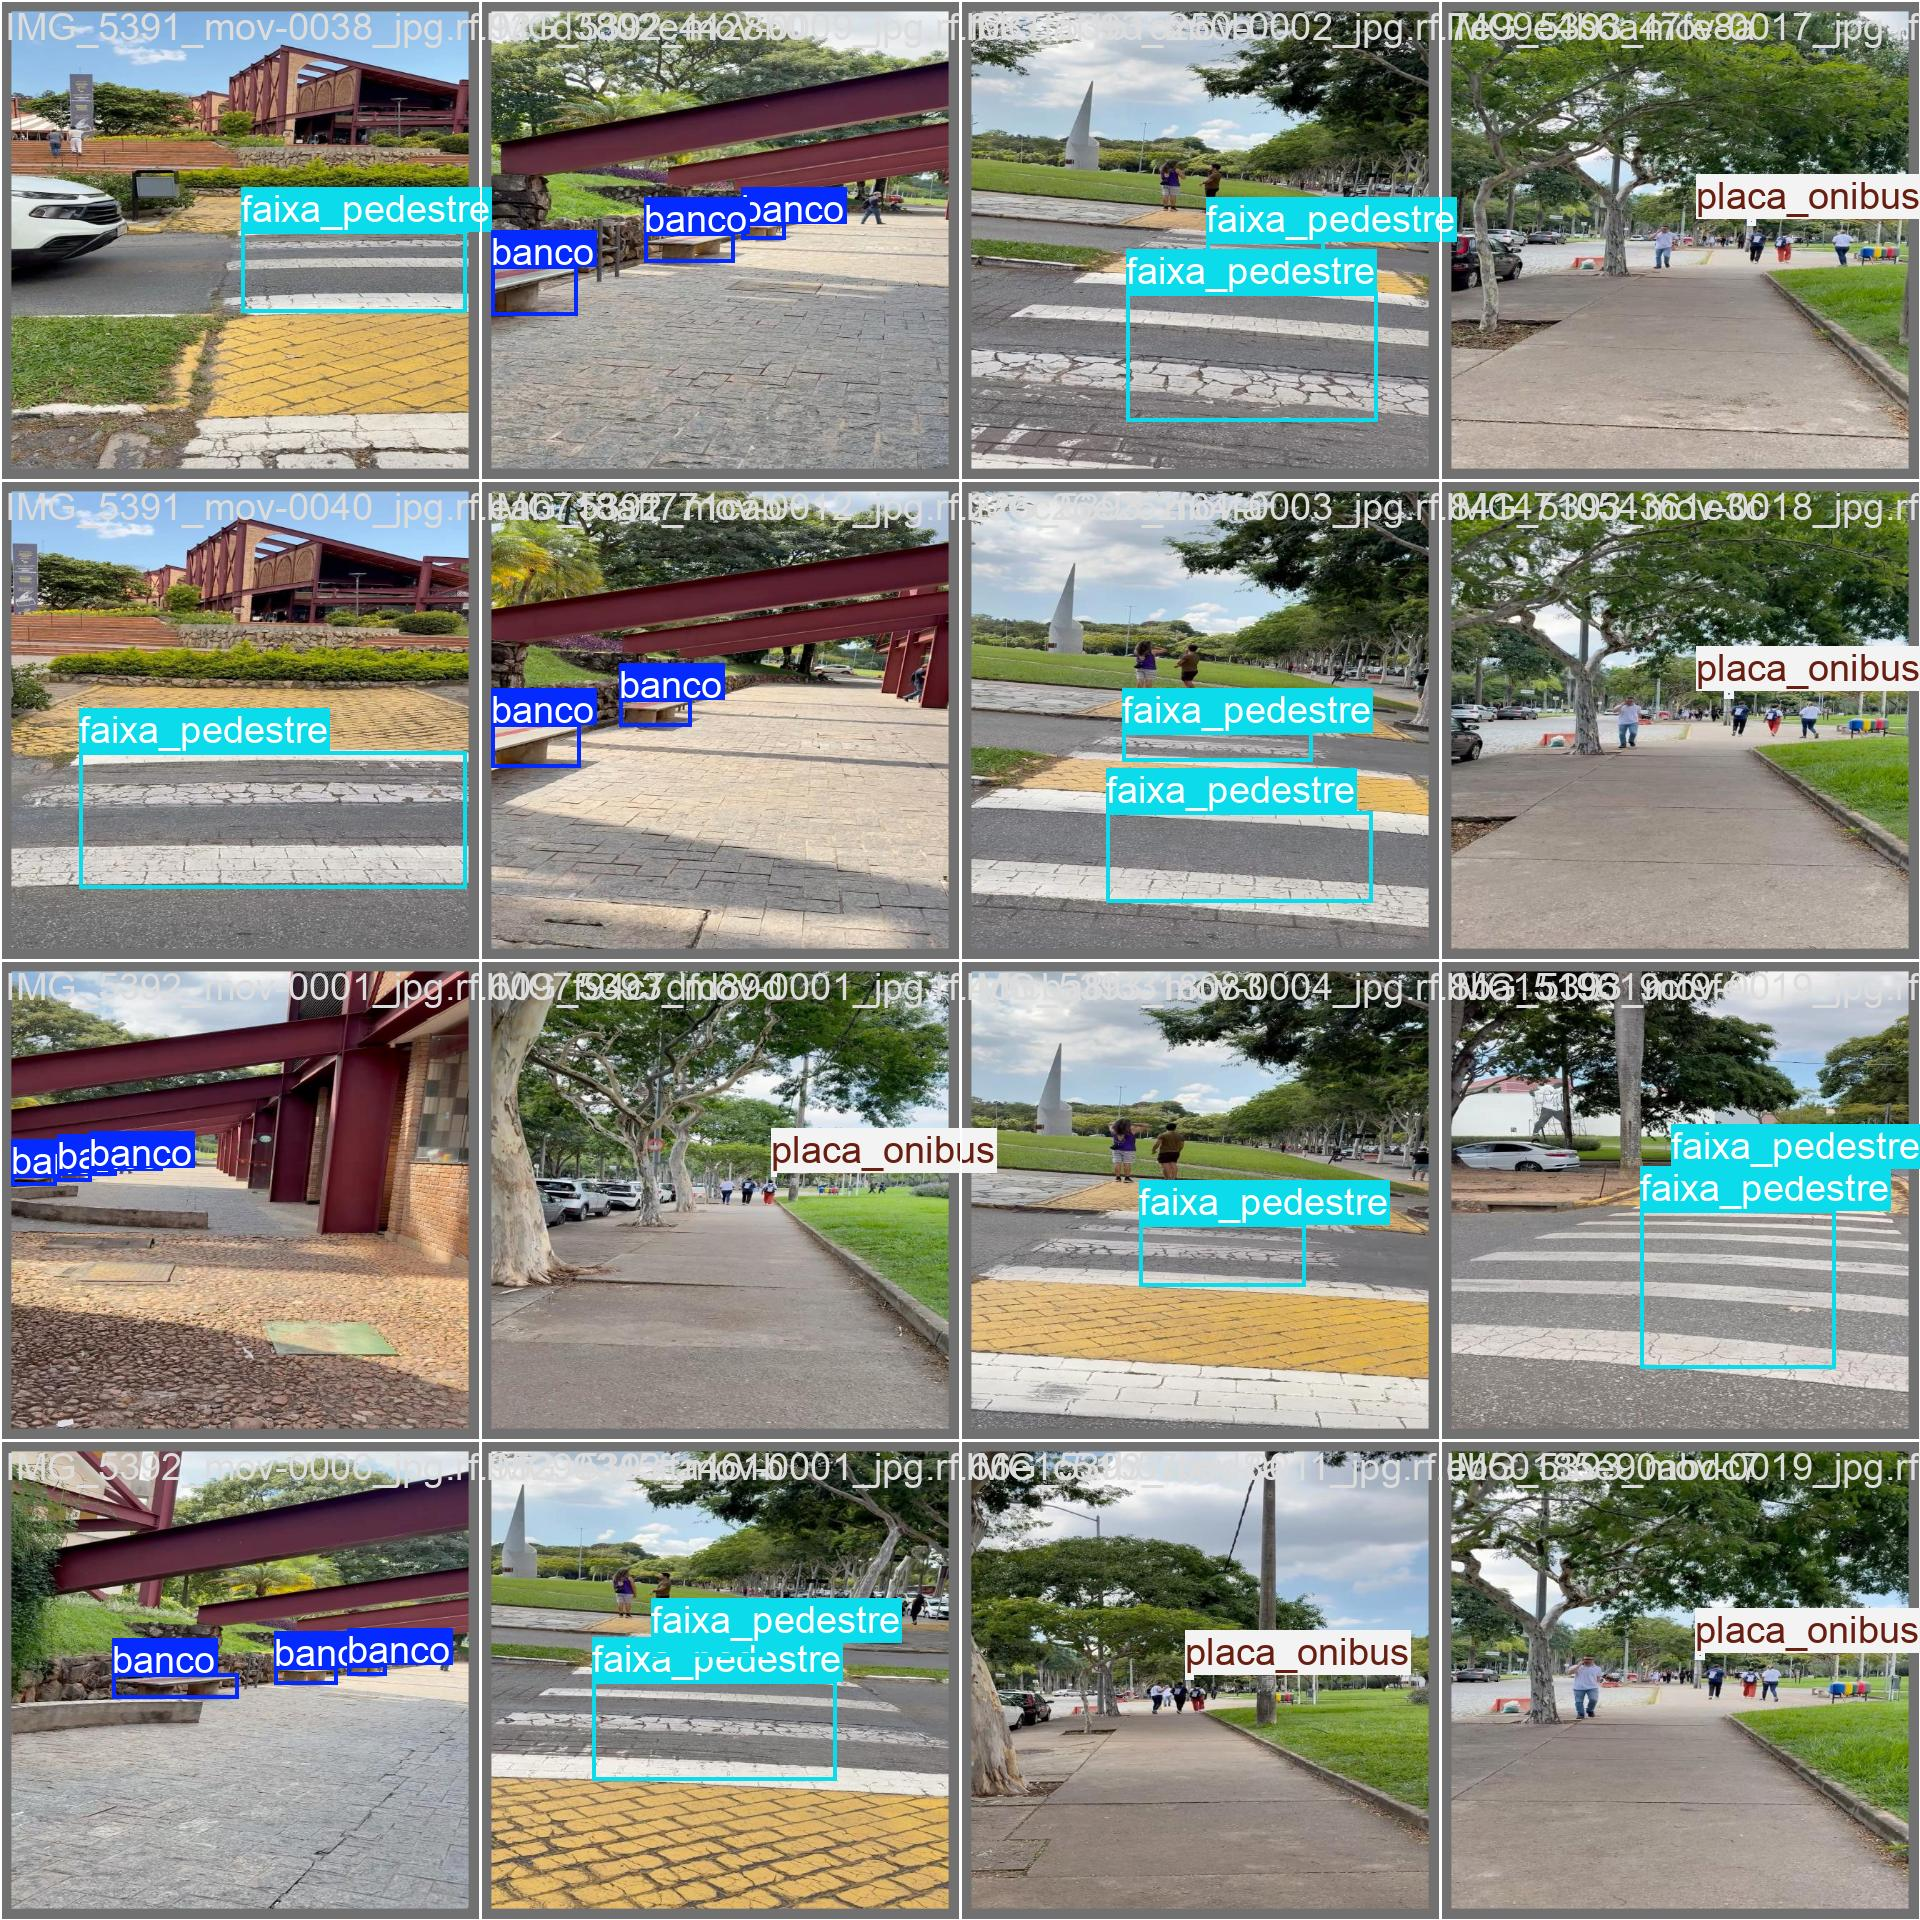
\includegraphics[width=1 \textwidth]{Figuras/val_batch2_labels.jpg}
  \\
  Fonte: Autoral.
  \label{fg-ex_anot3}
\end{figure}
% --- FIM Figura

Após a anotação, o dataset é expandido por meio de técnicas de \textit{data augmentation}, aplicando transformações como espelhamento, ajuste de brilho, saturação, ruído e \textit{blur}. Cada imagem gera três variações adicionais, elevando o número total para 1.444 imagens. Em seguida, os dados são redimensionados para 640x640 pixels e exportados no formato YOLO, com todos os arquivos organizados e enviados diretamente ao Google Colab via API.

A divisão final considera 88\% das imagens para treinamento e 12\% para validação, permitindo avaliar o desempenho durante o ajuste do modelo. A combinação de anotações precisas, variedade visual e aumentos realistas contribui para a robustez do modelo final, tornando essa etapa um dos pilares da qualidade do sistema proposto. A Figura \ref{fg-dataset-roboflow} ilustra o \textit{dataset} final na plataforma Roboflow.

% --- INÍCIO Figura
\begin{figure}[htbp]
  \centering
  \caption{Exemplo do \textit{dataset} final na plataforma Roboflow}
  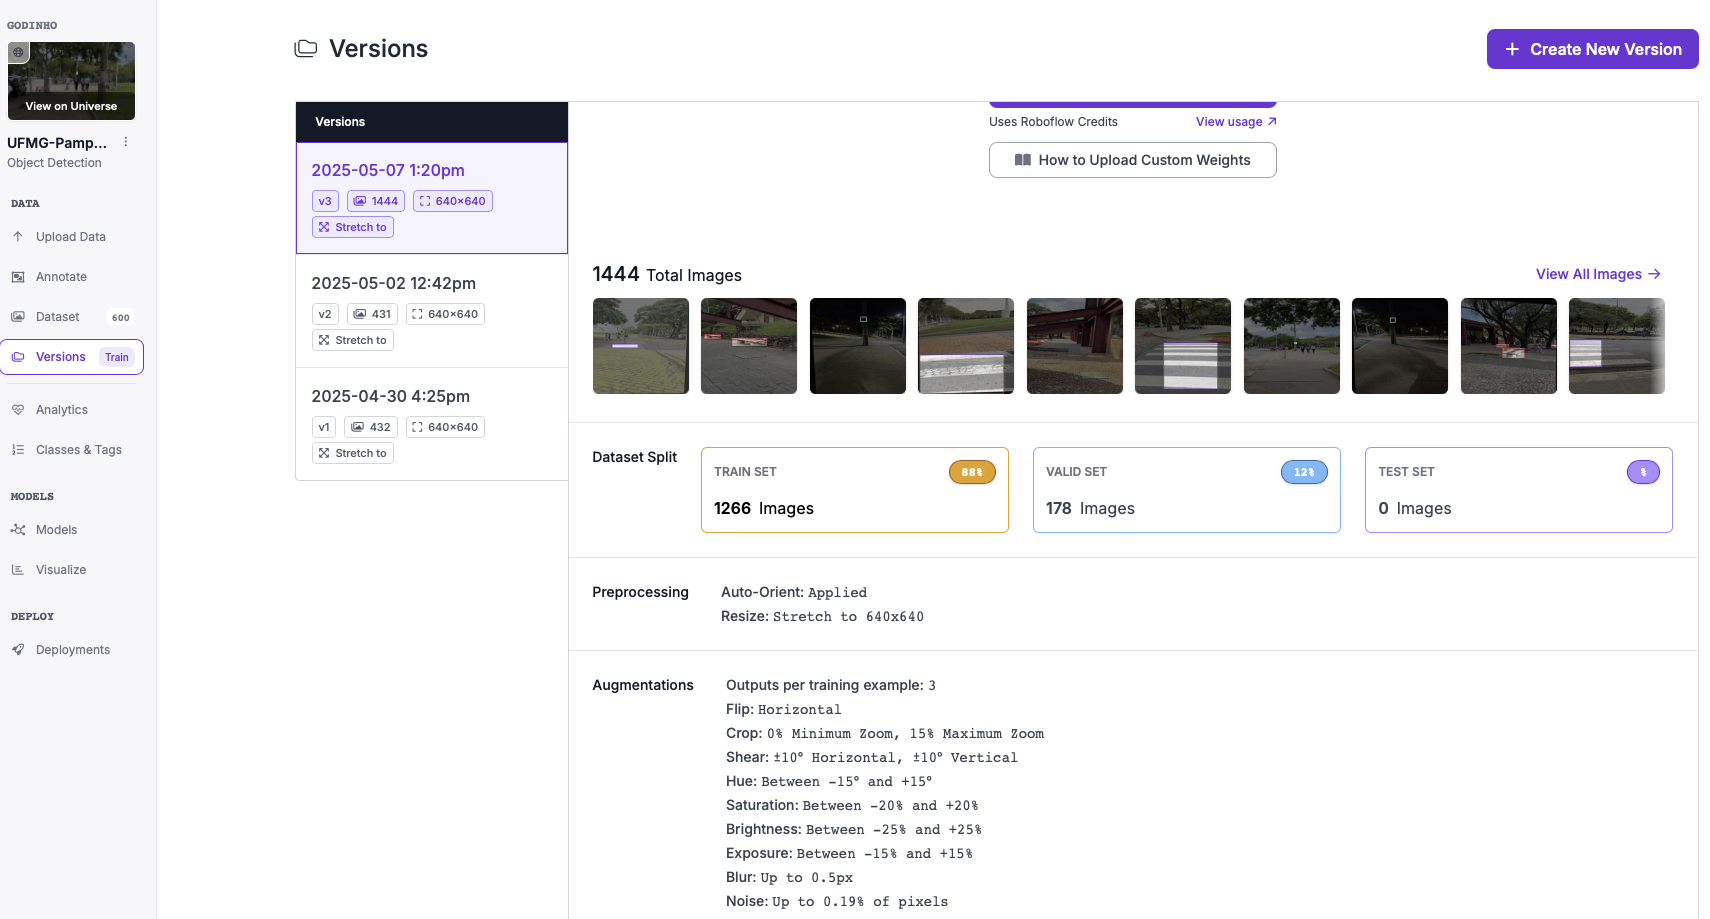
\includegraphics[width=1 \textwidth]{Figuras/dataset_roboflow.png}
  \\
  Fonte: Autoral.
  \label{fg-dataset-roboflow}
\end{figure}
% --- FIM Figura

\section{\textbf{Pré-processamento e \textit{Data Augmentation}}}

As etapas de pré-processamento e \textit{data augmentation} são executadas diretamente na plataforma Roboflow, com o objetivo de padronizar e diversificar as imagens do dataset. Todas as imagens são redimensionadas para 640×640 pixels, formato exigido pelo modelo YOLOv11, e passam por um processo automático de auto-orientação, que corrige a rotação de imagens capturadas em ângulos variados.

O processo de \textit{data augmentation} introduz variações sintéticas que simulam diferentes condições reais de iluminação, perspectiva e qualidade de captura. São aplicadas as seguintes transformações: \textit{flip} horizontal, \textit{zoom} com \textit{crop} (até 15\%), \textit{shear} horizontal e vertical (±10°), variações de brilho, exposição, matiz e saturação, além de \textit{blur} (até 0.5px) e ruído (até 0.19\%). Essas alterações visam aumentar a robustez do modelo frente a cenários não vistos durante o treinamento.

Cada imagem anotada gera três novas variações, aumentando o número de exemplos de forma significativa. A plataforma Roboflow garante que todas as \textit{bounding boxes} sejam ajustadas corretamente após cada transformação, mantendo a integridade dos dados anotados. O resultado é um dataset balanceado, diversificado e com anotações consistentes, pronto para ser exportado no formato YOLO, com arquivos .txt e data.yaml.

Esse aumento sintético permite ampliar a capacidade de generalização do modelo mesmo com uma base original limitada. A aplicação de \textit{augmentations} realistas contribui diretamente para o bom desempenho do sistema em ambientes com diferentes condições de iluminação, movimento e visibilidade, como será evidenciado nos resultados.

\section{\textbf{Treinamento do Modelo com o YOLOv11 personalizado}}

O modelo é treinado a partir da arquitetura YOLOv11, utilizando como base o yolo11m.pt, fornecido pela Ultralytics. Essa versão apresenta um bom equilíbrio entre precisão e velocidade de inferência, sendo adequada para dispositivos com recursos computacionais moderados.

O dataset é importado diretamente da Roboflow via API, contendo imagens, anotações e o arquivo data.yaml. O treinamento é iniciado com o seguinte comando padrão:

!yolo task=detect mode=train data=data.yaml model="yolo11m.pt" epochs=80\\imgsz=640 batch=-1

Esse comando define a tarefa de detecção, usa o modelo base YOLOv11m, executa 80 épocas de treinamento com imagens de 640×640 pixels e deixa o batch size em modo automático. O modelo ajusta seus pesos com base em \textit{backpropagation} e otimização por gradiente, monitorando continuamente as perdas de caixas delimitadoras (\textit{box\_loss}), classes (\textit{cls\_loss}) e distribuição de distância de focal (\textit{dfl\_loss}).

A cada época, o desempenho é validado com base nas métricas \textit{Precision}, \textit{Recall}, mAP@0.5 e mAP@0.5:0.95. O melhor modelo é salvo automaticamente na pasta /weights com o nome best.pt. O processo completo leva menos de 1 hora, com estabilidade nas curvas de perda e sem indícios de \textit{overfitting}, o que indica que o modelo está generalizando bem para os dados de validação.

\section{\textbf{Validação e Avaliação de Desempenho do Modelo}}

A validação é conduzida com 12\% do conjunto de dados reservados exclusivamente para esse fim. Esse subconjunto inclui imagens em diferentes horários do dia, com variações de iluminação, distância e presença de oclusões parciais. O objetivo é verificar a capacidade de generalização do modelo YOLOv11 treinado e mensurar seu desempenho em condições realistas de uso.

A execução da validação é feita com o seguinte comando padrão:

!yolo task=detect mode=val model=best.pt data=data.yaml split=val

Os resultados incluem métricas padrão: \textit{Precision} (0.921), \textit{Recall} (0.915), mAP@0.5 (0.944) e mAP@0.5:0.95 (0.672). A performance por classe também é satisfatória, com destaque para “placa\_onibus”, que atinge \textit{Precision} de 1.000 e \textit{Recall} de 0.997. A classe “banco” apresenta desempenho ligeiramente inferior (mAP@0.5:0.95 de 0.615), influenciada por oclusões e variações visuais nos vídeos.

O tempo médio de inferência é de 29,1 ms por imagem, com pré-processamento em torno de 4,0 ms e pós-processamento de 4,8 ms, demonstrando viabilidade para aplicações em tempo quase real. As curvas de perda e gráficos de desempenho gerados pela biblioteca Ultralytics mostram uma convergência estável sem indícios de overfitting. Também é realizada uma validação qualitativa com novos vídeos capturados no campus, confirmando a precisão das detecções em ambientes não vistos pelo modelo.

\section{\textbf{Testes em Vídeos Reais e Análise Qualitativa}}

Para avaliar o desempenho do sistema em condições reais de uso, são realizados testes com vídeos distintos dos utilizados no treinamento e validação. As gravações são feitas com o celular preso à altura do peito, simulando a perspectiva de um usuário durante o deslocamento no campus Pampulha da UFMG. Os testes abrangem diferentes horários do dia, condições de iluminação e variação de ocupação do ambiente.

A análise qualitativa baseia-se na observação visual das detecções renderizadas sobre os vídeos. São avaliados a estabilidade das \textit{bounding boxes}, a consistência na classificação dos objetos e a robustez diante de oclusões, movimentações no cenário e variações de luz. O modelo mantém boa performance geral, com confiabilidade superior a 0.85 em grande parte dos quadros para as classes placa\_onibus e faixa\_pedestre. A classe banco apresenta maior sensibilidade a obstáculos visuais, como presença de pessoas ou vegetação.

Além das detecções visuais, também é testado o funcionamento do sistema de geração de alertas sonoros. Os áudios, sincronizados aos vídeos, transmitem informações contextuais com clareza e precisão. A integração entre detecção visual e feedback auditivo reforça o potencial da ferramenta para aplicações assistivas, demonstrando fluidez na comunicação com o usuário.

As limitações observadas incluem quedas na confiança durante cenas noturnas ou com iluminação artificial intensa, além de falhas pontuais na detecção de objetos em ângulos extremos. Apesar disso, os testes confirmam que o sistema é funcional em contextos diversos, com desempenho robusto e usabilidade promissora, servindo como prova de conceito viável para aplicações futuras em tempo real.

\section{\textbf{Geração de \textit{Feedback} Auditivo a partir das Detecções}}

Nesta etapa, o sistema converte as detecções visuais em mensagens sonoras, possibilitando que pessoas com deficiência visual compreendam a presença e a localização de objetos no ambiente. A conversão é feita com a biblioteca gTTS, que transforma textos em áudios no idioma português. A cada detecção válida, o sistema gera frases como “faixa de pedestre à frente” ou “banco à esquerda”, que são sincronizadas com o vídeo correspondente.

Para determinar a posição dos objetos, o sistema divide cada \textit{frame} em três regiões verticais (esquerda, centro e direita), com base no ponto central da \textit{bounding box} detectada. Um deslocamento percentual de 15\% dos \textit{pixels} a partir do centro define os limites laterais. A partir da classe e da posição, o sistema concatena a string da mensagem que será convertida em áudio.

O áudio gerado é sincronizado com os frames do vídeo utilizando a biblioteca MoviePy, enquanto o módulo de \textit{debouncing} evita repetição de alertas em posições semelhantes em curto intervalo de tempo. Os limiares de repetição são ajustados conforme a classe: placas de ponto de ônibus e faixas exigem maior espaçamento, enquanto bancos admitem menor intervalo.

O processamento final gera um vídeo com detecções visuais sobrepostas e alertas sonoros integrados, simulando o uso real do sistema. Toda a implementação é feita em Python, com as bibliotecas Ultralytics, OpenCV, gTTS, MoviePy, NumPy e logging. O código está disponível no GitHub\footnote{\url{https://github.com/Matheus-Godinho-Magalhaes/Final_Paper}} e modularizado para facilitar manutenção e reuso. O resultado demonstra que o sistema é capaz de traduzir informações visuais em mensagens acessíveis, aproximando-se de uma solução funcional de tecnologia assistiva.

\section{\textbf{Considerações Éticas e Limitações da Implementação}}

A coleta de dados visuais é realizada exclusivamente em áreas públicas do campus Pampulha da UFMG, com foco em objetos de interesse definidos previamente. O projeto evita a identificação de pessoas e não armazena dados sensíveis. Em casos em que indivíduos aparecem incidentalmente nos vídeos, não ocorre qualquer tentativa de reconhecimento facial ou extração de informações pessoais, e as imagens são utilizadas apenas para treinamento interno do modelo.

A proposta busca ampliar a acessibilidade para pessoas com deficiência visual, respeitando diretrizes éticas e legais. A solução é concebida como uma ferramenta de baixo custo, com potencial para ser embarcada em dispositivos móveis e adaptada a outros contextos institucionais ou urbanos. A finalidade do sistema é exclusivamente assistiva, sem coleta de dados do usuário ou uso comercial das imagens.

Entre as principais limitações, destaca-se o fato de que o sistema opera com vídeos pré-gravados, e não em tempo real. Isso impede seu uso imediato como ferramenta interativa e exige processamento posterior para gerar os alertas. A implementação em tempo real requer dispositivos com maior capacidade computacional e ajustes na integração com câmeras em execução contínua. Além disso, o modelo é treinado com dados específicos do campus da UFMG, o que pode reduzir sua precisão em outros contextos, como ruas urbanas ou outras instituições.

Variações ambientais, como baixa iluminação, obstruções visuais e mudanças climáticas, também impactam a confiabilidade do sistema. O posicionamento da câmera no corpo do usuário pode gerar distorções na detecção, exigindo padronização ou mecanismos adaptativos. Embora os testes realizados indiquem bons resultados, a validação com usuários reais ainda é necessária para aferir a clareza dos alertas, o conforto auditivo e a efetividade da solução em situações cotidianas.

\section{\textbf{Considerações Finais}}

Este trabalho adota uma abordagem aplicada e experimental, com foco na construção de uma solução funcional voltada à assistência de pessoas com deficiência visual no campus da UFMG. A proposta parte de um problema real e busca resolvê-lo com o uso de tecnologias existentes, integradas de forma prática, iterativa e mensurável.

A metodologia desenvolvida segue uma lógica incremental, em que cada etapa, desde a coleta dos dados até a geração de feedback auditivo, contribui de forma objetiva para a composição de um sistema funcional. O modelo treinado é testado com vídeos reais, anotados manualmente, e os resultados são validados por métricas quantitativas e por testes qualitativos em condições variadas de uso. Essa abordagem permite verificar não apenas a precisão algorítmica, mas também a adequação funcional do sistema no ambiente-alvo.

Do ponto de vista técnico, o trabalho se destaca por utilizar ferramentas de código aberto e infraestrutura gratuita (Google Colab, Roboflow, Ultralytics), promovendo reprodutibilidade, acessibilidade e escalabilidade. As decisões metodológicas priorizam a clareza, a leveza computacional e a adaptabilidade a diferentes contextos futuros, mesmo com recursos limitados.

Por fim, o trabalho propõe mais do que um experimento acadêmico: apresenta uma prova de conceito concreta, replicável e socialmente relevante. A estratégia adotada demonstra que é possível construir sistemas assistivos eficientes com tecnologias atuais e acessíveis, desde que com planejamento metodológico sólido e foco nas reais necessidades do público-alvo.
\chapter{\textbf{ANÁLISE E RESULTADOS}}
\section{\textbf{Introdução à Análise de Resultados}}

Este capítulo apresenta a análise e discussão dos resultados obtidos no desenvolvimento do sistema de detecção de objetos e espaços no campus Pampulha da UFMG, com foco em sua aplicação como ferramenta assistiva para pessoas com deficiência visual. A avaliação tem como principal objetivo verificar a eficácia do modelo yolo11m.pt treinado com um \textit{dataset} personalizado, considerando tanto aspectos quantitativos quanto qualitativos do seu desempenho.

A análise está estruturada com base em artefatos gerados ao longo das fases de treinamento e validação do modelo, dentre os quais se destacam os gráficos de evolução das métricas durante as épocas, matrizes de confusão, curvas de \textit{precision}-\textit{recall}, medidas consolidadas de desempenho e exemplos visuais de detecção. Estes elementos possibilitam uma compreensão abrangente da capacidade do modelo em reconhecer corretamente as classes de interesse, banco, faixa de pedestre e placa de ônibus, sob diferentes condições ambientais.

Inicialmente, o capítulo aborda a caracterização do \textit{dataset} utilizado, detalhando sua composição e distribuição das classes. Em seguida, são analisadas as curvas de aprendizado do modelo, com foco na convergência das funções de perda e evolução das métricas. Na sequência, são apresentados os resultados quantitativos consolidados, seguidos por uma investigação mais minuciosa de erros e acertos por classe. Também são discutidas as relações entre o limiar de confiança e o comportamento das métricas de desempenho, com o auxílio de curvas \textit{Precision}-\textit{Recall} (PR) e \textit{F1-Score} (F1).

Complementarmente à análise numérica, são incluídas observações qualitativas baseadas em detecções reais em vídeos e imagens, buscando evidenciar situações práticas de acerto, erro e limitação do sistema. Por fim, é realizada uma discussão integrada dos resultados, com reflexões sobre o potencial do modelo como componente central de uma solução assistiva.

\section{\textbf{Caracterização do \textit{Dataset} e Configuração Detalhada do Treinamento}}

A qualidade e a representatividade do conjunto de dados são fatores determinantes para o desempenho de modelos baseados em aprendizado profundo, especialmente em aplicações de visão computacional. O \textit{dataset} utilizado neste trabalho foi construído com imagens capturadas no campus Pampulha da UFMG, abrangendo diferentes condições de luminosidade, horários do dia e contextos de ocupação do espaço. O objetivo foi garantir diversidade suficiente para permitir a generalização do modelo frente às variações ambientais do local de aplicação.

Foram definidas três classes de interesse, selecionadas com base em sua relevância para a orientação e segurança de pessoas com deficiência visual no contexto universitário: banco, faixa de pedestre e placa de ponto de ônibus. A distribuição dessas classes está ilustrada na Figura \ref{fg-labels}, com destaque para a predominância da classe banco, seguida por faixa de pedestre e, por fim, placa de ônibus. Embora o número de instâncias não seja equilibrado entre as classes, todas foram representadas em quantidade suficiente para permitir o aprendizado, considerando as boas práticas para \textit{datasets} personalizados de detecção de objetos.

% --- Figura
\begin{figure}[htbp]
  \centering
  \caption{Análise da distribuição das anotações e distribuição espacial das caixas delimitadoras no \textit{dataset}.}
  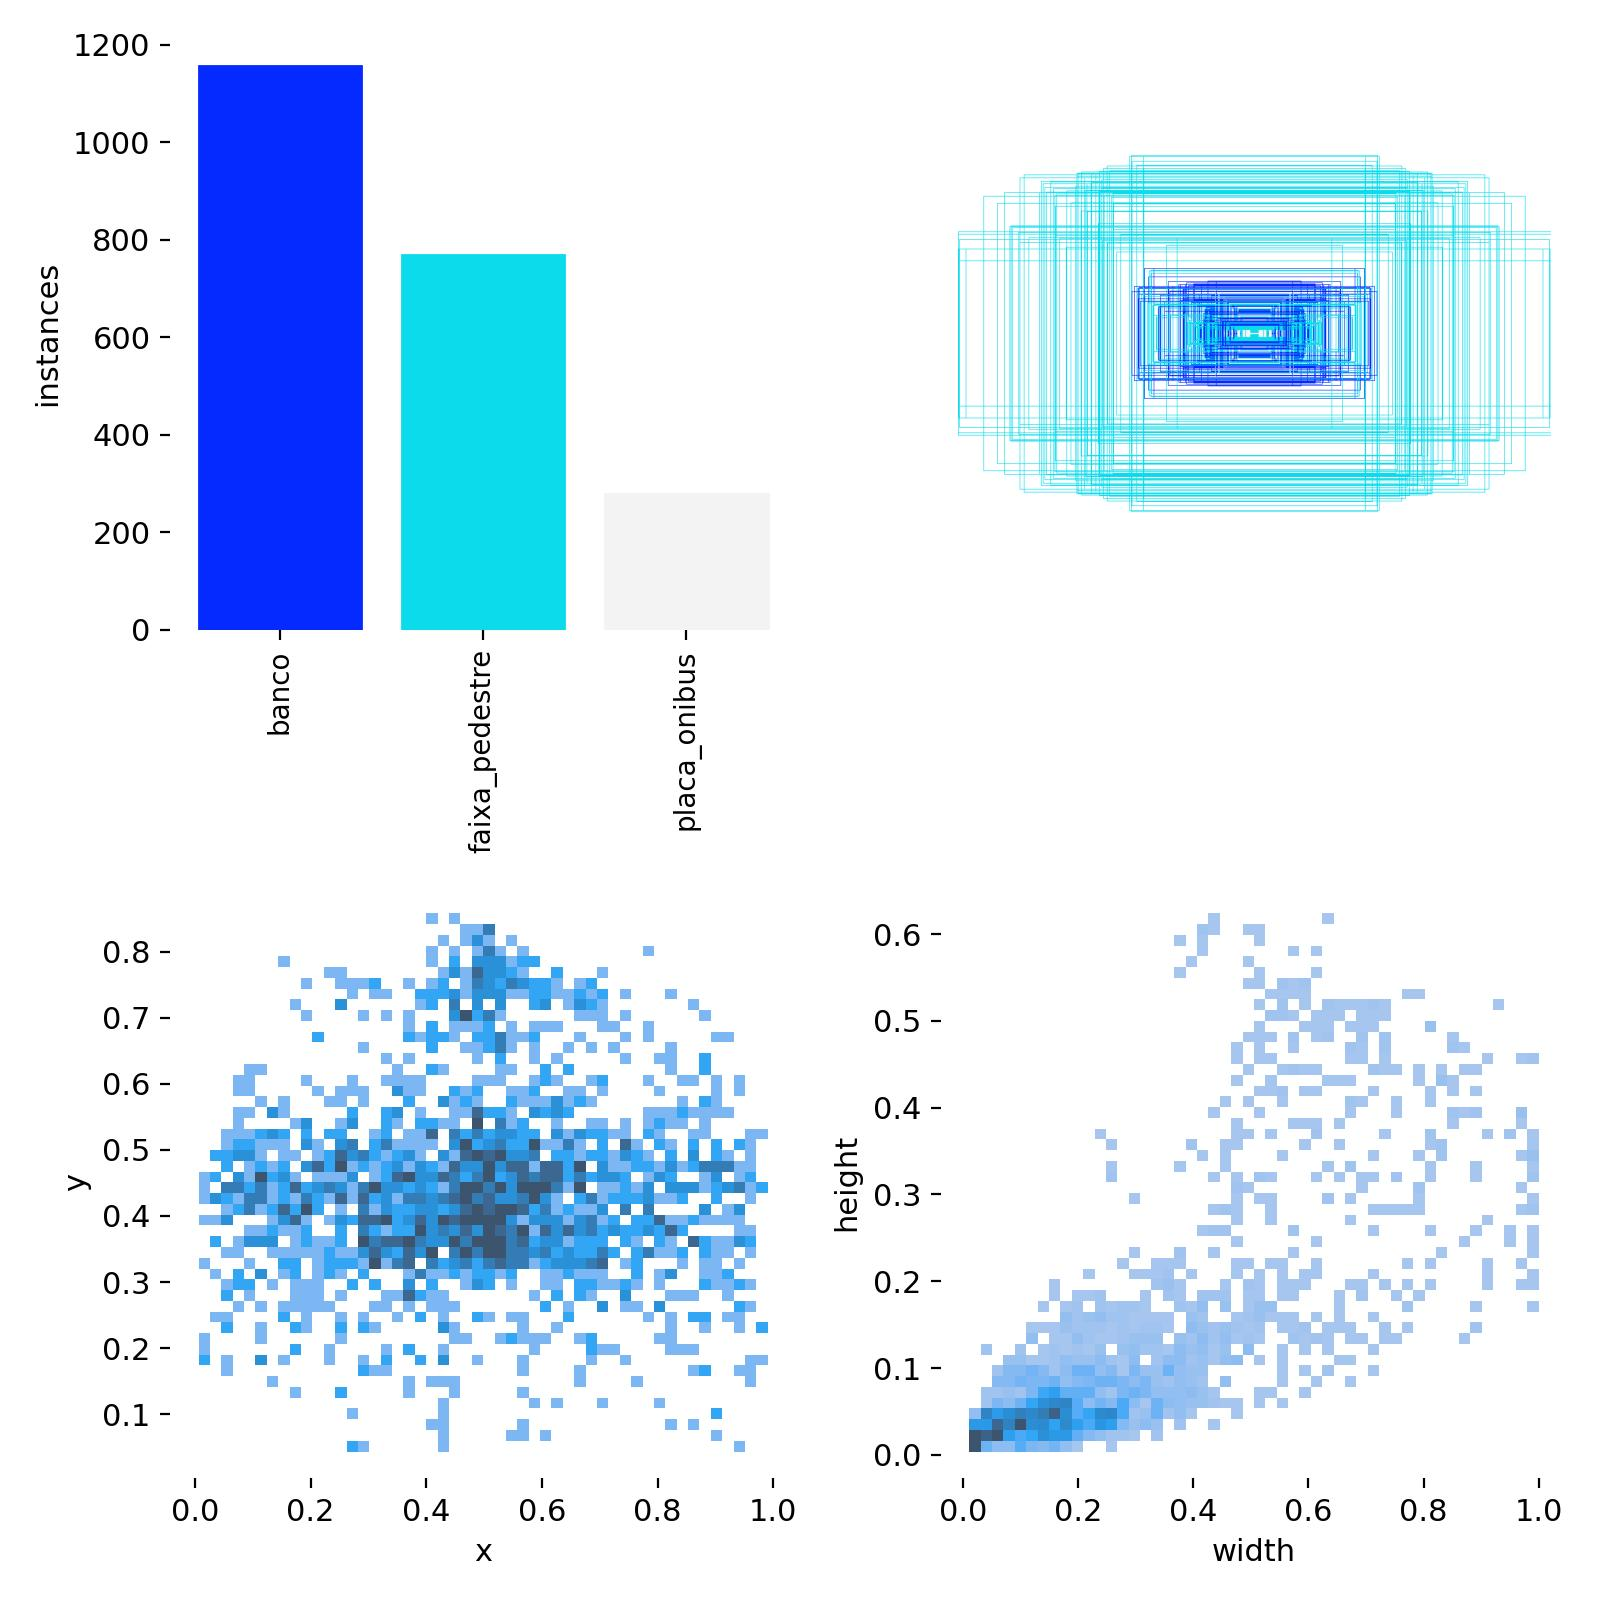
\includegraphics[width=0.8\textwidth]{Figuras/labels.jpg}
  \\
  Fonte: Autoral.
  \label{fg-labels}
\end{figure}
% --- Figura

A fim de aumentar a variabilidade das amostras e reduzir o risco de \textit{overfitting}, foi aplicada uma estratégia de \textit{data augmentation}, incluindo técnicas como espelhamento horizontal, ajustes de brilho e saturação, inserção de ruído e pequenas transformações geométricas. Com isso, o número total de imagens disponíveis para o treinamento foi expandido de aproximadamente 600 para 1444. Adicionalmente, as anotações foram realizadas de forma detalhada com auxílio da plataforma Roboflow, que também foi responsável pela divisão do \textit{dataset} em 88\% para o conjunto de treinamento e 12\% para validação.

A distribuição espacial das anotações nos \textit{frames} indica que os objetos foram capturados em diferentes posições e tamanhos dentro da imagem, o que é desejável para a aprendizagem de um detector robusto. A variedade nas dimensões e localizações das caixas delimitadoras reforça a heterogeneidade do conjunto, permitindo ao modelo aprender a identificar os objetos independentemente de sua escala, orientação ou posição no campo visual.

O processo de treinamento foi conduzido com base na arquitetura YOLOv11, utilizando pesos pré-treinados (modelo yolo11m.pt) como ponto de partida. A execução ocorreu em ambiente Google Colab, com o uso de uma GPU NVIDIA Tesla T4. As imagens foram redimensionadas para 640x640 pixels, e o treinamento estendeu-se por 80 épocas. A escolha automática do tamanho de batch (definido como -1) resultou em lotes de 14 imagens, considerando as limitações da GPU disponível.

A configuração dos hiperparâmetros foi gerenciada pela biblioteca Ultralytics, com a seleção automática do otimizador AdamW e de uma taxa de aprendizado ajustável. Essa automatização visou otimizar o processo para os recursos computacionais disponíveis e acelerar a convergência do modelo. A Figura \ref{fg-labels} também apresenta a distribuição dos centros e tamanhos das caixas, reforçando a diversidade de exemplos que alimentaram o processo de aprendizado.

Em síntese, a construção criteriosa do \textit{dataset} e a configuração adequada do processo de treinamento formaram uma base sólida para os resultados apresentados nas seções subsequentes. A diversidade de cenários contemplados, aliada ao uso de técnicas de \textit{data augmentation}, contribuiu significativamente para a robustez do modelo treinado frente às condições reais de aplicação no ambiente universitário.

\section{\textbf{Análise do Processo de Convergência do Modelo durante o Treinamento}}

A análise das curvas de convergência durante o treinamento do modelo yolo11m.pt fornece informações essenciais sobre a eficácia do processo de aprendizado e sobre a estabilidade das métricas de desempenho ao longo das épocas. A Figura \ref{fg-results} compila os gráficos gerados pela biblioteca Ultralytics, apresentando a evolução das funções de perda e métricas de \textit{precision} e \textit{recall} tanto para o conjunto de treinamento quanto para o conjunto de validação.

% --- Figura
\begin{figure}[htbp]
  \centering
  \caption{Evolução das métricas de perda (box, cls, dfl) e \textit{Mean Average Precision} (mAP50, mAP50-95) nos conjuntos de treinamento (linha superior) e validação (linha inferior) ao longo das 80 épocas de treinamento do modelo}
  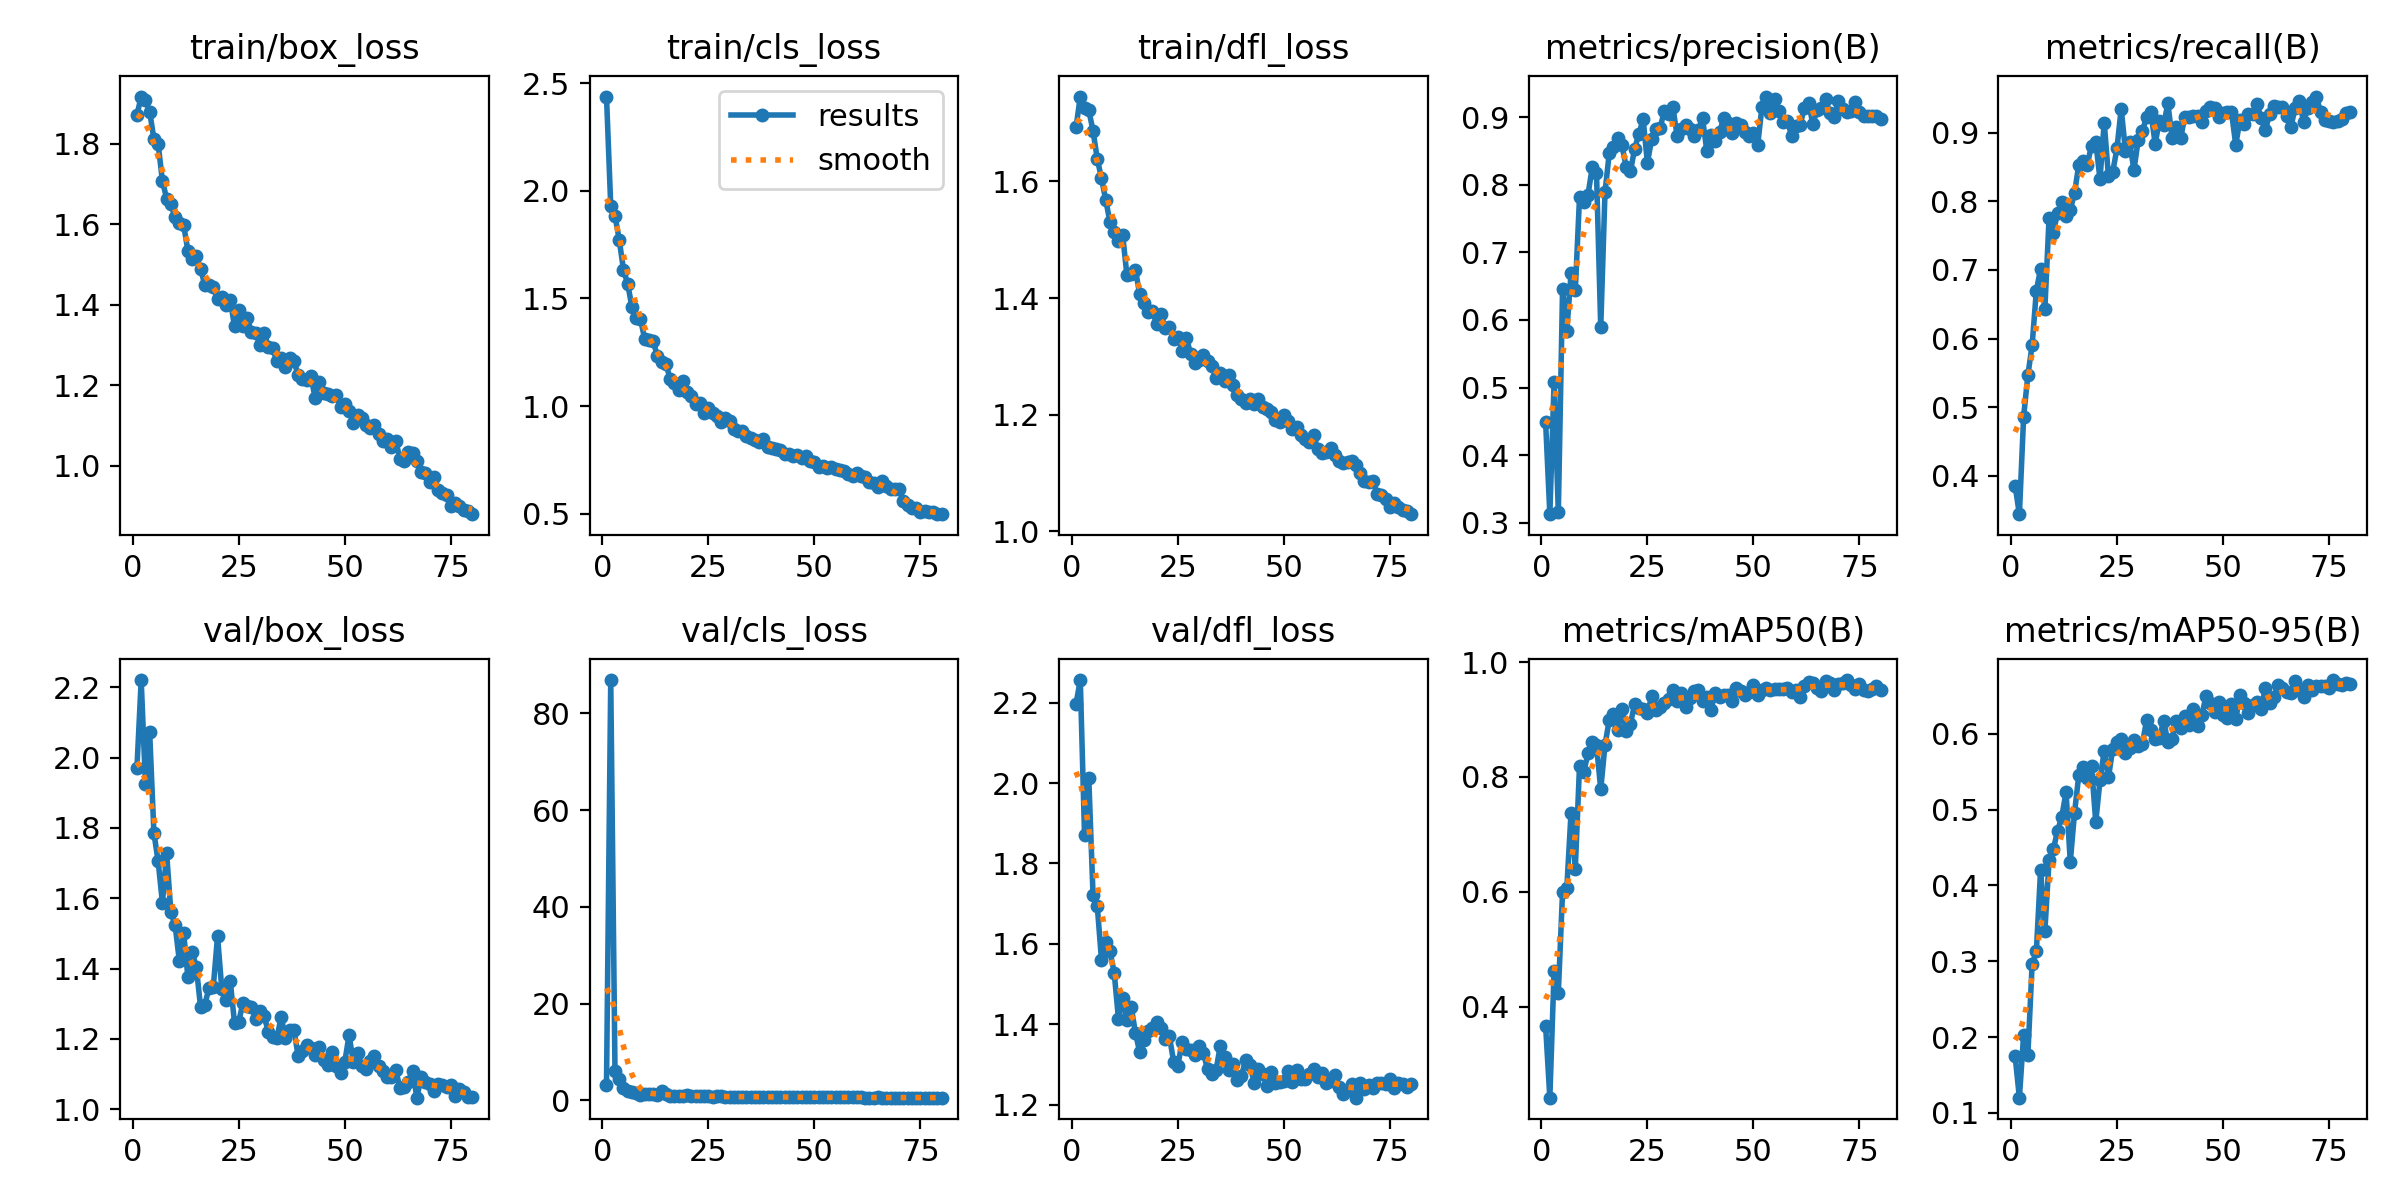
\includegraphics[width=1\textwidth]{Figuras/results.png}
  \\
  Fonte: Autoral.
  \label{fg-results}
\end{figure}
% --- Figura

Observa-se nas curvas de perda (\textit{box\_loss}, \textit{cls\_loss} e \textit{dfl\_loss}) um comportamento típico de convergência eficiente: redução acentuada nas primeiras 30 épocas, seguida de estabilização progressiva até aproximadamente a 75ª época. Este padrão é evidência de que o modelo ajustou adequadamente seus parâmetros iniciais, entrando posteriormente em uma fase de refinamento gradual. A ausência de oscilações abruptas ou aumentos nas curvas de perda valida a consistência do processo e a adequação da taxa de aprendizado empregada.

As curvas referentes ao conjunto de validação acompanham de forma coesa as do treinamento, sem divergências significativas entre elas. Essa proximidade indica que o modelo não sofreu \textit{overfitting} durante as 80 épocas, mantendo sua capacidade de generalização para dados não vistos. A semelhança entre os comportamentos dos dois conjuntos também sugere que as técnicas de regularização adotadas, aliadas à diversidade do \textit{dataset}, foram eficazes para a estabilização do processo.

Em relação às métricas de desempenho, destacam-se os valores progressivamente crescentes de mAP@0.5 e mAP@0.5:0.95. A métrica mAP@0.5 ultrapassou o valor de 0.90 antes da 50ª época, estabilizando-se em torno de 0.94 nas últimas iterações. Já a métrica mAP@0.5:0.95, mais rigorosa, apresentou crescimento contínuo, atingindo valores superiores a 0.70. Ambos os resultados são indicadores de desempenho elevado, considerando-se o contexto de aplicação e o volume de dados utilizados.

As métricas de \textit{precision} e \textit{recall} apresentaram curvas consistentes com o comportamento das perdas. Em particular, o \textit{recall} manteve-se elevado ao longo das últimas épocas, evidenciando a capacidade do modelo de detectar a maioria dos objetos presentes nas imagens. A \textit{precision}, por sua vez, apresentou estabilidade após a 40ª época, refletindo o equilíbrio alcançado entre acertos e falsos positivos.

Conclui-se, com base nas curvas de aprendizado e desempenho, que o modelo convergiu de forma eficaz dentro do intervalo estipulado de 80 épocas. A ausência de comportamento instável, a aproximação entre os conjuntos de treinamento e validação e os altos valores de mAP consolidam a confiabilidade do processo de treinamento, justificando a seleção do modelo gerado como base para as avaliações quantitativas e qualitativas posteriores.

\section{\textbf{Avaliação Quantitativa de Desempenho do Modelo Final}}

Finalizado o treinamento, o modelo yolo11m.pt foi avaliado por meio da aplicação do conjunto de pesos otimizados (arquivo best.pt) sobre o subconjunto de validação do \textit{dataset}, contendo 178 imagens e 306 instâncias. Essa validação foi conduzida com a ferramenta Ultralytics, utilizando o comando específico em modo val, responsável por calcular as métricas consolidadas de desempenho para cada classe. Os resultados estão organizados na Tabela \ref{tab:metricas-yolov11m}, que resume as métricas de \textit{precision}, \textit{recall}, mAP@0.5 e mAP@0.5:0.95 por classe e no total.

\begin{table}[htbp]
\centering
\caption{Métricas de desempenho do modelo \texttt{yolo11m.pt} (best.pt) no conjunto de validação}
\label{tab:metricas-yolov11m}
\resizebox{\textwidth}{!}{%
\begin{tabular}{lcccccc}
\toprule
\textbf{Classe} & \textbf{Imagens} & \textbf{Instâncias} & \textbf{\textit{Precision}} (P) & \textbf{\textit{Recall}} (R) & \textbf{mAP@0.5} & \textbf{mAP@0.5:0.95} \\
\midrule
Todas (média)   & 178               & 306                 & 0.927                 & 0.936               & 0.967            & 0.670               \\
Banco           & 67               & 152                  & 0.859                 & 0.941               & 0.942            & 0.681               \\
Faixa\_pedestre & 86               & 104                  & 0.921                 & 0.893               & 0.966            & 0.606               \\
Placa\_onibus   & 50               & 50                  & 1.000                 & 0.973               & 0.994            & 0.721               \\
\bottomrule
\end{tabular}%
}
\end{table}

A análise da média geral evidencia um desempenho expressivo do modelo. A \textit{precision} de 0.927 indica que, entre todas as detecções realizadas, aproximadamente 93\% foram corretas. O \textit{recall} de 0.936 demonstra que o modelo conseguiu identificar a grande maioria dos objetos presentes nas imagens. A métrica mAP@0.5, com valor de 0.967, confirma a alta acurácia da detecção com uma tolerância padrão de Intersecção sobre União (IoU) de 50\%. Já a mAP@0.5:0.95, com valor de 0.670, representa um resultado satisfatório mesmo sob critérios mais rígidos de correspondência entre predição e anotação.


No desempenho individual por classe, destaca-se a classe placa\_onibus, que atingiu \textit{precision} perfeita de 1.000, \textit{recall} de 0.973 e mAP@0.5:0.95 de 0.721 — o melhor entre todas as classes. Este resultado sugere que o modelo identificou com segurança e exatidão as placas de ponto de ônibus, possivelmente devido ao seu formato e cor característicos, que oferecem menor ambiguidade visual.

A classe faixa\_pedestre apresentou resultados igualmente positivos, com \textit{precision} de 0.921 e \textit{recall} de 0.893. O mAP@0.5 de 0.966 reflete o bom desempenho na detecção e delimitação espacial deste tipo de objeto, apesar de sua variabilidade de aparência e iluminação, especialmente sob diferentes condições de piso e sombra.

Já a classe banco, embora com métricas consideradas aceitáveis, apresentou o desempenho mais modesto. A \textit{precision} de 0.859 e o \textit{recall} de 0.941 indicam maior incidência de falsos positivos e negativos em relação às demais classes. O valor de mAP@0.5 de 0.942 confirma essa maior dificuldade, atribuível à diversidade de formas, tamanhos e materiais dos bancos encontrados no campus, além de sua frequente oclusão parcial por pessoas ou vegetação.

Ressalta-se que o conjunto de validação utilizado é limitado em tamanho, o que pode introduzir certa variabilidade estatística nos resultados. Ainda assim, os padrões observados são consistentes com as análises das curvas de treinamento (Figura \ref{fg-results}) e com as tendências verificadas na matriz de confusão (próxima seção). A velocidade de inferência, próxima de 23 ms por imagem na GPU Tesla T4, também reforça a viabilidade do modelo para aplicações em tempo real.

Em resumo, os resultados quantitativos obtidos confirmam que o modelo yolo11m.pt treinado apresenta desempenho compatível com aplicações práticas de suporte à navegação assistiva, oferecendo boa acurácia de detecção, baixo índice de erro e estabilidade frente a dados não vistos.

\section{\textbf{Análise Detalhada de Erros e Acertos com Base na Matriz de Confusão}}

A matriz de confusão é uma ferramenta essencial para a avaliação detalhada do desempenho de modelos de classificação, permitindo a identificação dos padrões de acertos e erros em cada classe individualmente. No contexto do modelo, essa análise revela não apenas a eficácia do algoritmo na classificação correta dos objetos, mas também os pontos de maior vulnerabilidade, especialmente no que diz respeito à distinção entre objetos de interesse e o fundo (\textit{background}).

A Figura \ref{fg-confusion_matrix} apresenta a matriz de confusão bruta, evidenciando a contagem absoluta das classificações feitas pelo modelo durante a validação. Os valores ao longo da diagonal principal indicam as classificações corretas, ou seja, os verdadeiros positivos (TP) para cada classe. Os valores fora da diagonal, por sua vez, representam erros de classificação, como falsos positivos (FP) e falsos negativos (FN). Observa-se que o modelo não apresentou confusões entre as classes-alvo, como por exemplo classificar um banco como faixa de pedestre. Isso demonstra uma clara capacidade discriminativa entre as classes definidas no \textit{dataset} personalizado.

% --- Figura
\begin{figure}[htbp]
  \centering
  \caption{Matriz de Confusão com contagens absolutas das predições no conjunto de validação do treinamento do modelo}
  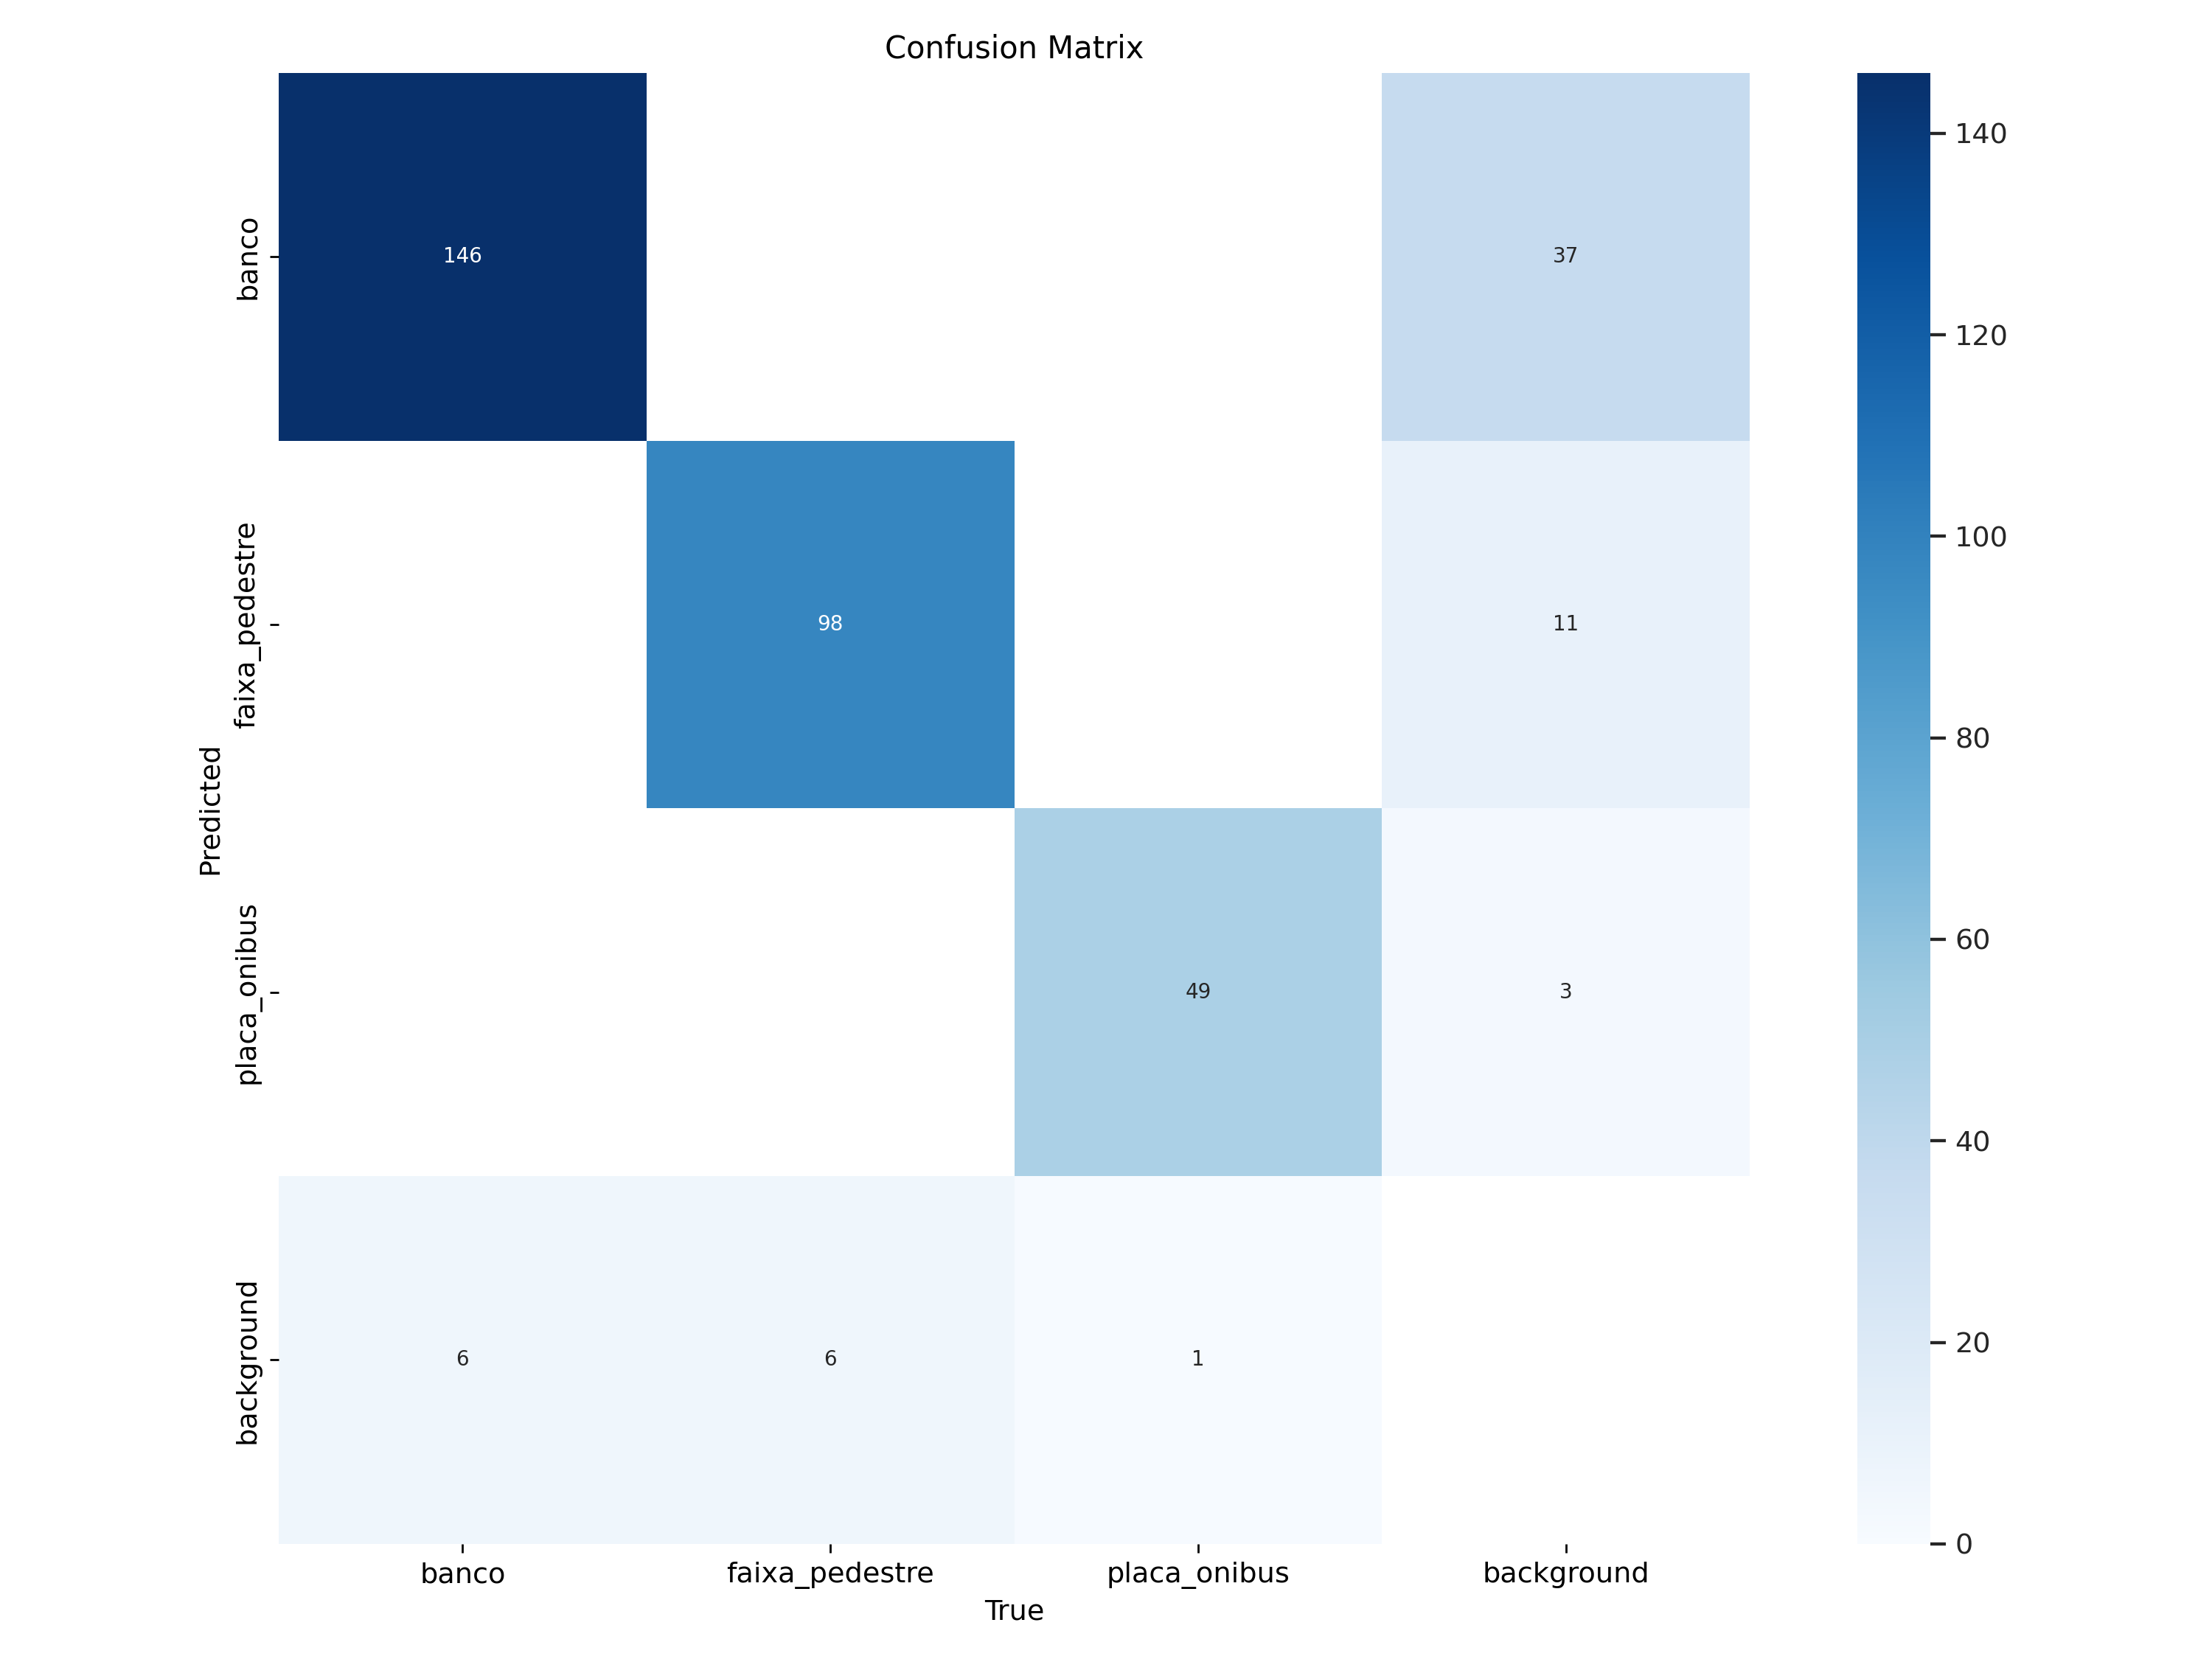
\includegraphics[width=1\textwidth]{Figuras/confusion_matrix.png}
  \\
  Fonte: Autoral.
  \label{fg-confusion_matrix}
\end{figure}
% --- Figura

No entanto, as maiores ocorrências de erros concentram-se na relação com o \textit{background}. Foram observados 37 falsos positivos para a classe banco, 11 para faixa\_pedestre e apenas 3 para placa\_onibus. Isso indica que o modelo, em algumas situações, interpretou elementos visuais do ambiente como objetos de interesse, quando na realidade tratava-se de elementos do cenário não anotados. Tais erros podem ser atribuídos a texturas ou estruturas visuais semelhantes aos objetos de interesse, como sombras, muros ou áreas pavimentadas com padrões similares.

A análise da matriz de confusão normalizada (Figura \ref{fg-confusion_matrix_normalized}) oferece uma visualização mais intuitiva do \textit{recall} por classe, ou seja, a proporção de objetos reais corretamente identificados pelo modelo. Os resultados indicam um desempenho elevado: banco com 96\%, faixa\_pedestre com 9\% e placa\_onibus com 98\%. Esses valores confirmam que o modelo possui uma elevada sensibilidade, sendo capaz de detectar a maioria dos objetos de cada categoria. Os erros restantes (FN) são geralmente atribuídos a condições adversas, como baixa iluminação, oclusões ou aparências incomuns dos objetos.

% --- Figura
\begin{figure}[htbp]
  \centering
  \caption{Matriz de Confusão Normalizada (valores da diagonal representam o \textit{Recall} por classe)}
  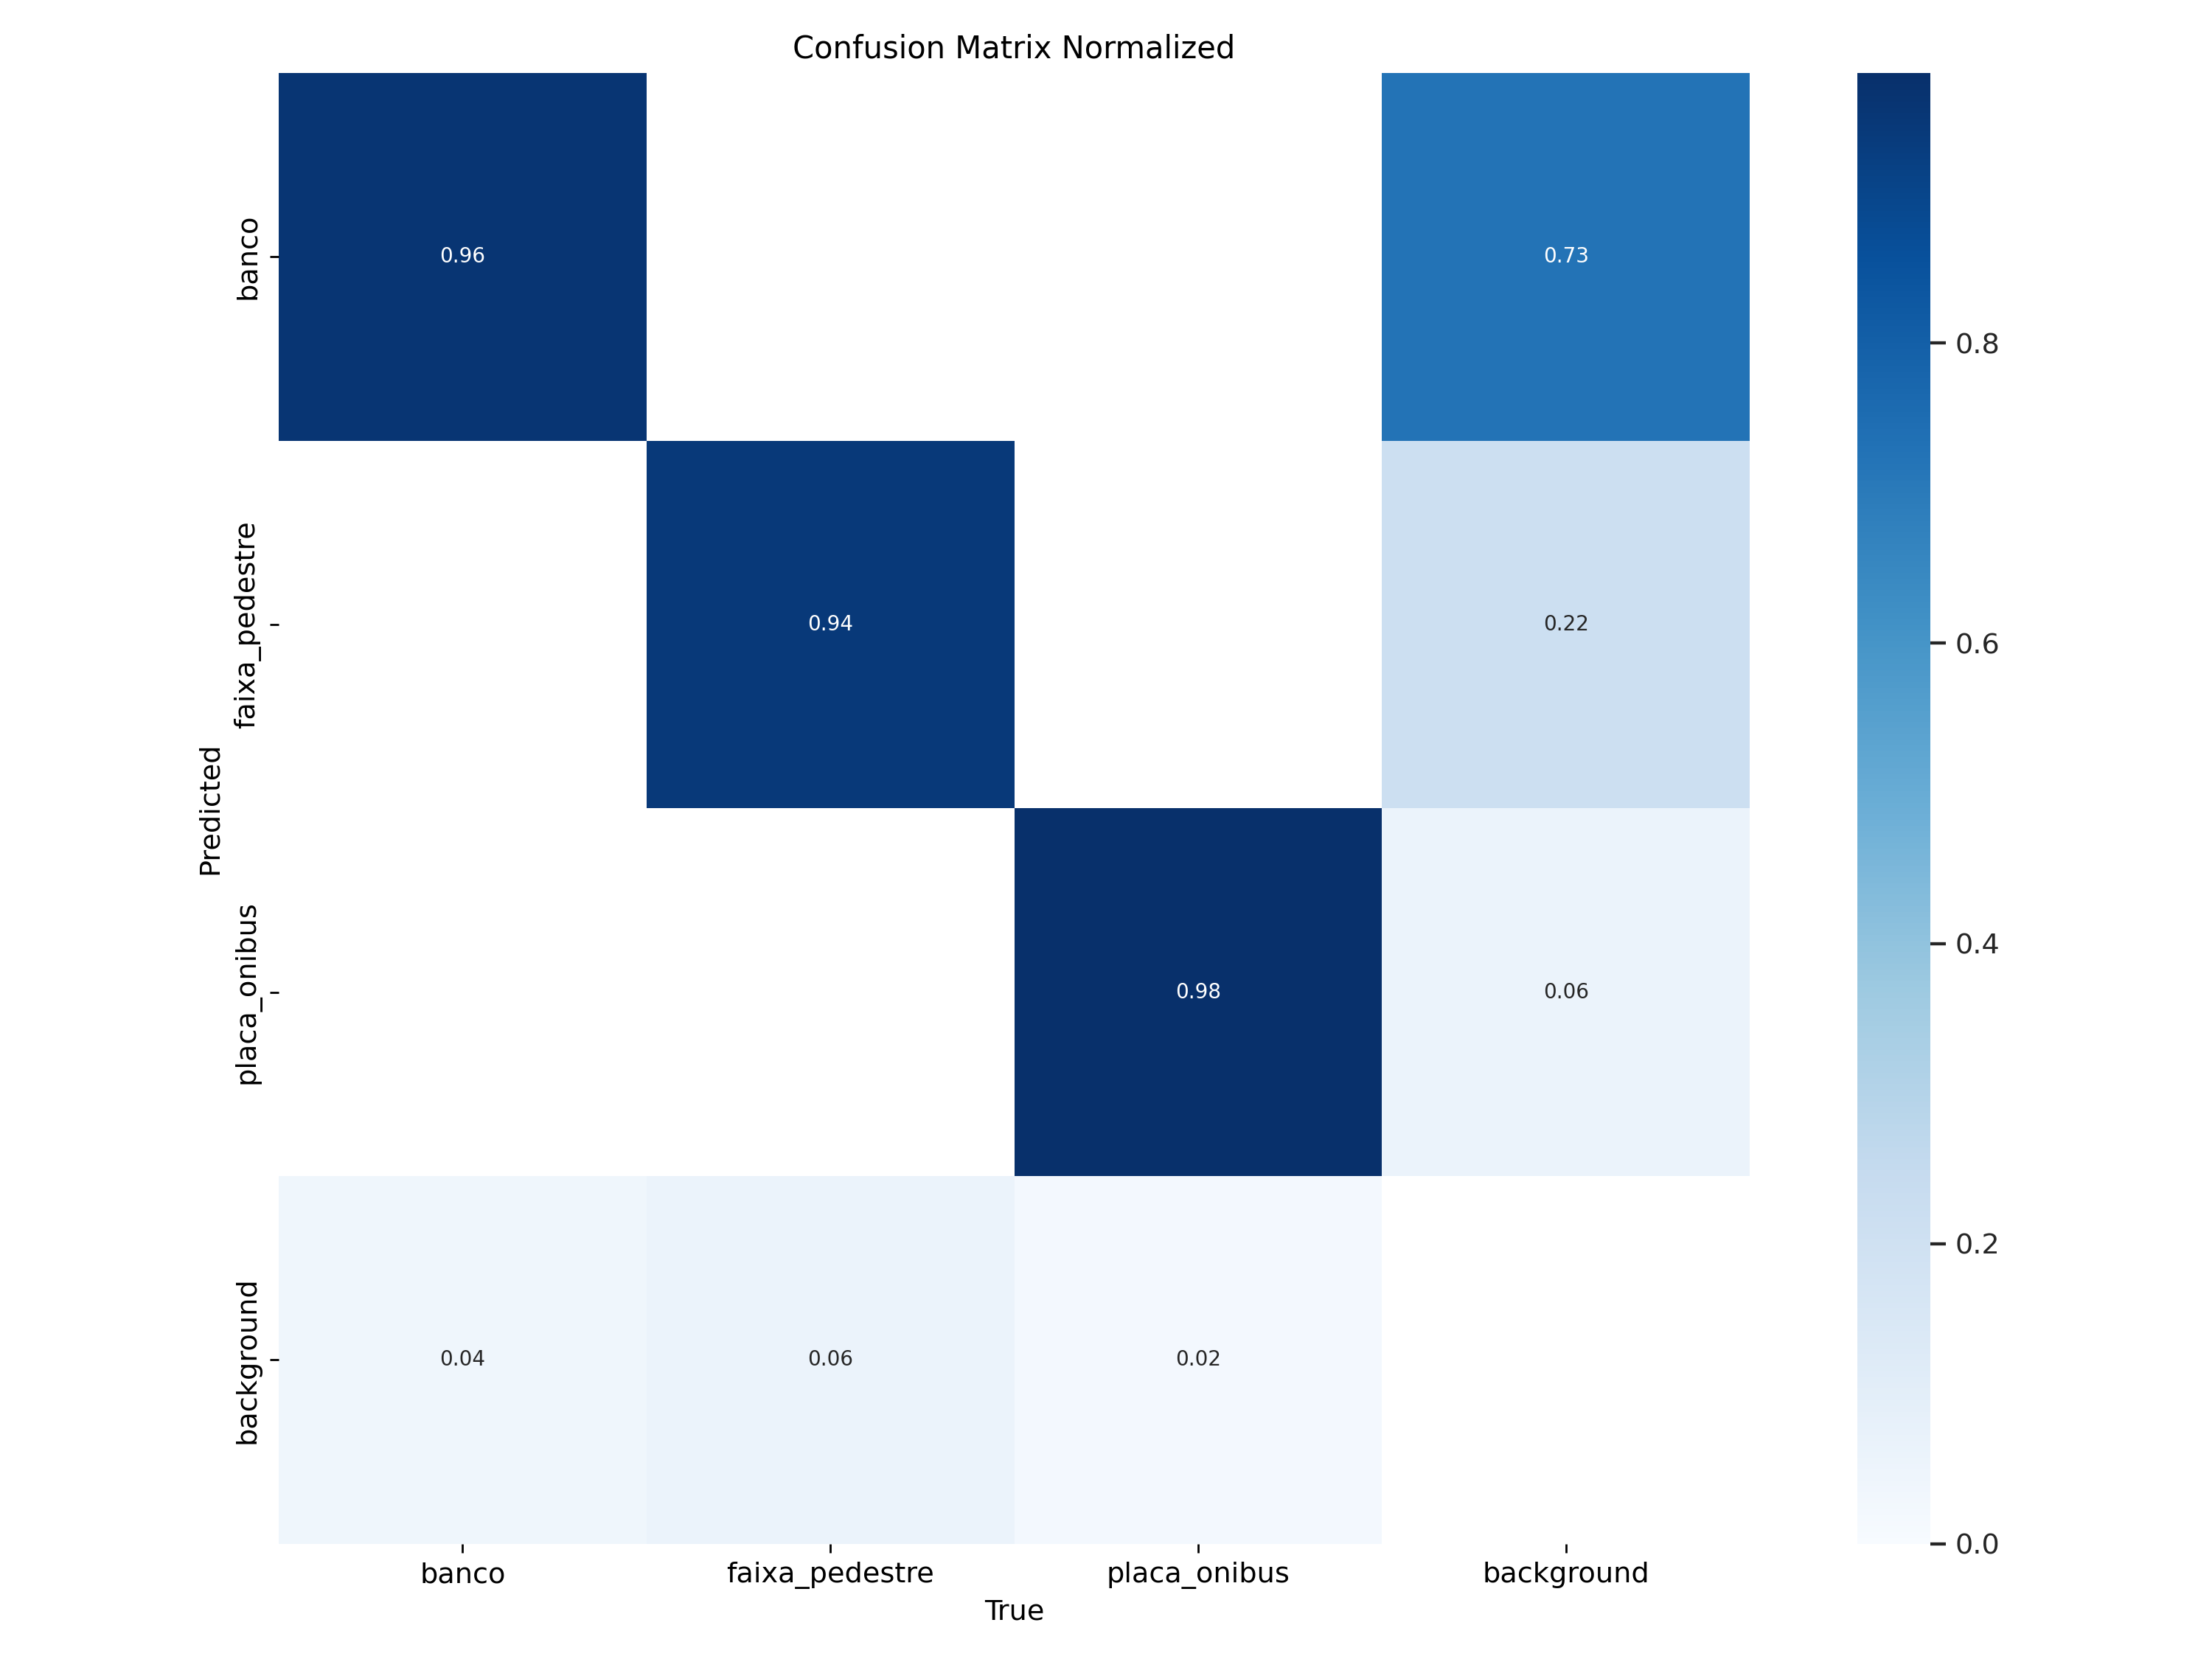
\includegraphics[width=1\textwidth]{Figuras/confusion_matrix_normalized.png}
  \\
  Fonte: Autoral.
  \label{fg-confusion_matrix_normalized}
\end{figure}
% --- Figura

A classe banco, apesar de apresentar um bom desempenho geral, foi a que mais acumulou falsos positivos. Isso sugere a necessidade de refinamento adicional, seja por meio da inclusão de exemplos negativos (\textit{background}s semelhantes a bancos) no \textit{dataset}, seja pela calibragem mais cuidadosa do limiar de confiança durante a inferência. Essa medida pode ajudar a minimizar alertas incorretos na aplicação final assistiva, sem comprometer o \textit{recall} da classe.

Em síntese, a análise das matrizes de confusão reforça que o modelo é confiável para aplicações práticas, demonstrando altos índices de acerto e baixa taxa de confusão entre classes. As limitações identificadas são pontuais e passíveis de aprimoramento, sem comprometer a viabilidade da ferramenta assistiva.


\section{\textbf{Relação entre Limiar de Confiança, \textit{Precision}, \textit{Recall} e \textit{F1-Score}}}

O desempenho de modelos de detecção de objetos é influenciado diretamente pelo limiar de confiança utilizado na inferência. Esse parâmetro define o grau mínimo de certeza que o modelo deve ter para considerar uma detecção como válida. Assim, ajustes nesse valor afetam diretamente o equilíbrio entre \textit{precision} (proporção de detecções corretas entre as detectadas) e \textit{recall} (proporção de detecções corretas entre as existentes). A análise das curvas PR e F1 permite entender essa dinâmica de maneira visual e quantitativa.

A Figura \ref{fg-pr_curve} apresenta as curvas PR para cada uma das classes, bem como para a média geral do modelo. Essas curvas ilustram o comportamento da \textit{precision} em função do aumento do \textit{recall}. Curvas que se mantêm próximas do canto superior direito do gráfico indicam um desempenho superior, com alta \textit{precision} mesmo quando o \textit{recall} é elevado. No presente modelo, observou-se que todas as classes apresentam curvas com esse comportamento desejável, com destaque para a classe placa\_onibus, que manteve \textit{precision} elevada em quase toda a faixa de \textit{recall}.

% --- Figura
\begin{figure}[htbp]
  \centering
  \caption{Curvas \textit{Precision}-\textit{Recall} para cada classe e para a média de todas as classes (mAP@0.5) no conjunto de validação do treinamento do modelo}
  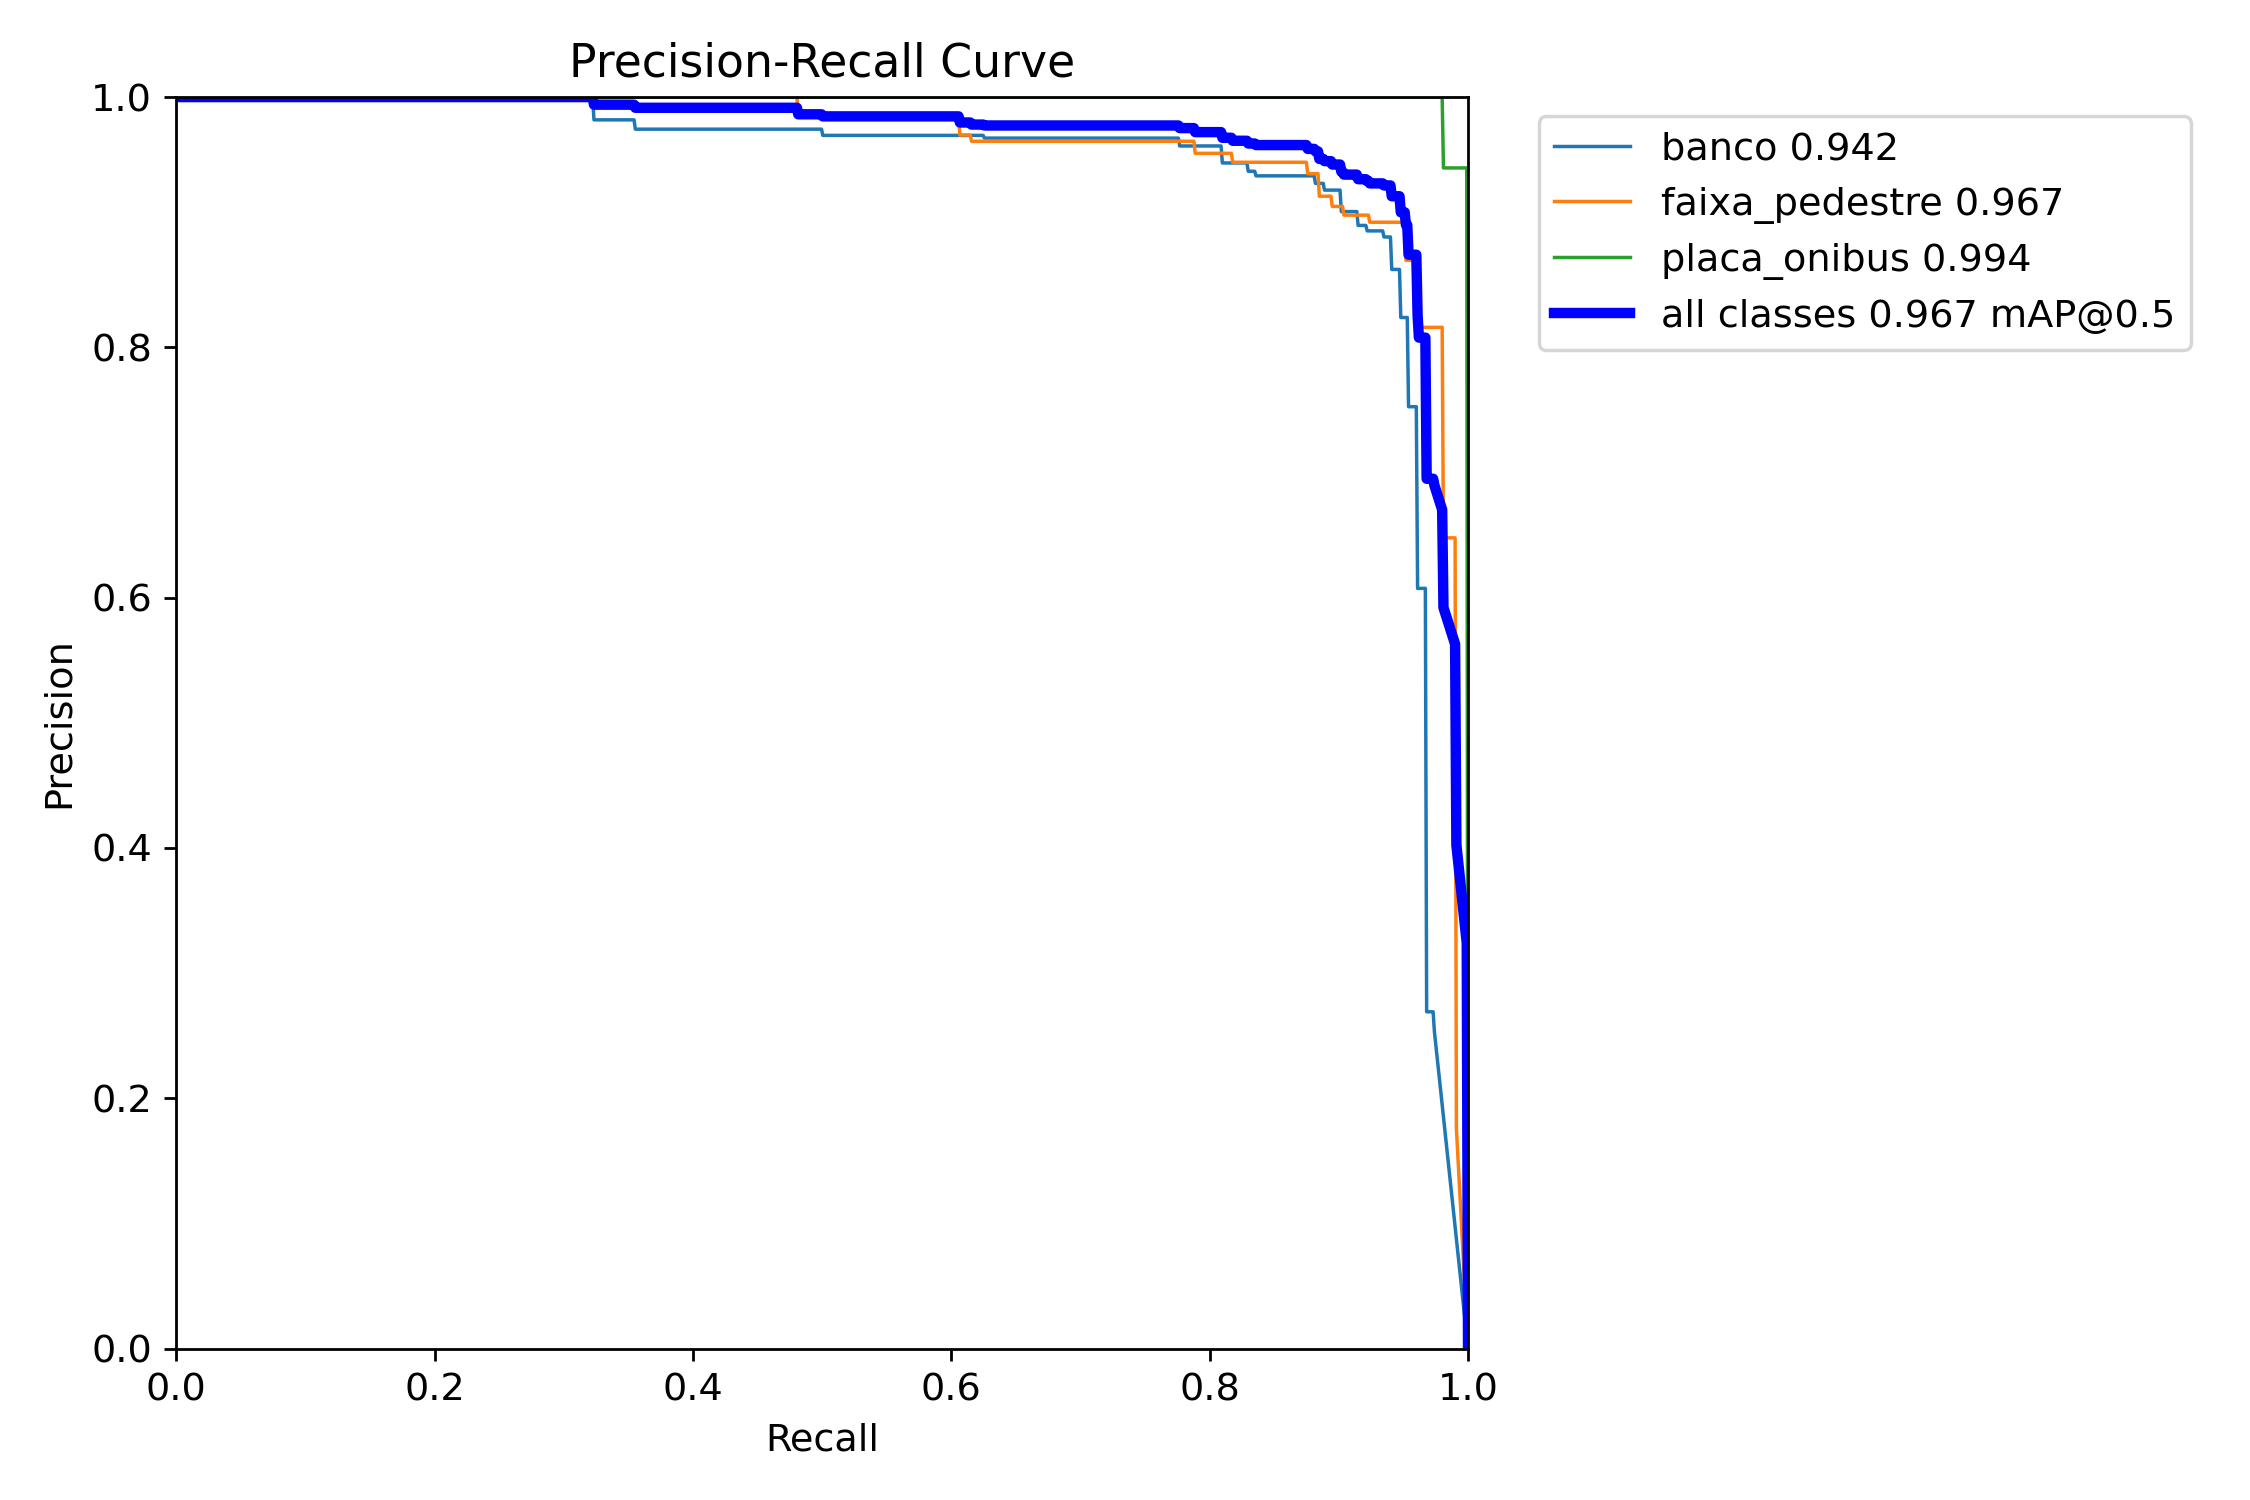
\includegraphics[width=1\textwidth]{Figuras/PR_curve.png}
  \\
  Fonte: Autoral.
  \label{fg-pr_curve}
\end{figure}
% --- Figura

Os valores de \textit{average precision} (AP) extraídos das curvas são bastante expressivos: 0.942 para banco, 0.967 para faixa\_pedestre e 0.994 para placa\_onibus. Esses resultados refletem a alta eficácia do modelo, especialmente considerando que foram obtidos com um \textit{dataset} personalizado e em ambiente não controlado. O AP médio de 0.967 indica que o modelo mantém um equilíbrio adequado entre \textit{precision} e \textit{recall} na maioria das situações.

A Figura \ref{fg-f1_curve} complementa a análise ao mostrar o comportamento do \textit{F1-Score} em função do limiar de confiança. O \textit{F1-Score} é uma métrica harmônica entre \textit{precision} e \textit{recall}, sendo especialmente útil para identificar o ponto ótimo de operação do modelo. Observa-se que o ponto de \textit{F1-Score} máximo para o modelo geral ocorre em torno de um limiar de 0.404, indicando que esse valor proporciona o melhor equilíbrio entre detectar objetos corretamente e evitar detecções incorretas.

% --- Figura
\begin{figure}[htbp]
  \centering
  \caption{Curvas do \textit{F1-Score} em função do Limiar de Confiança para cada classe e para a média de todas as classes no conjunto de validação do treinamento do modelo}
  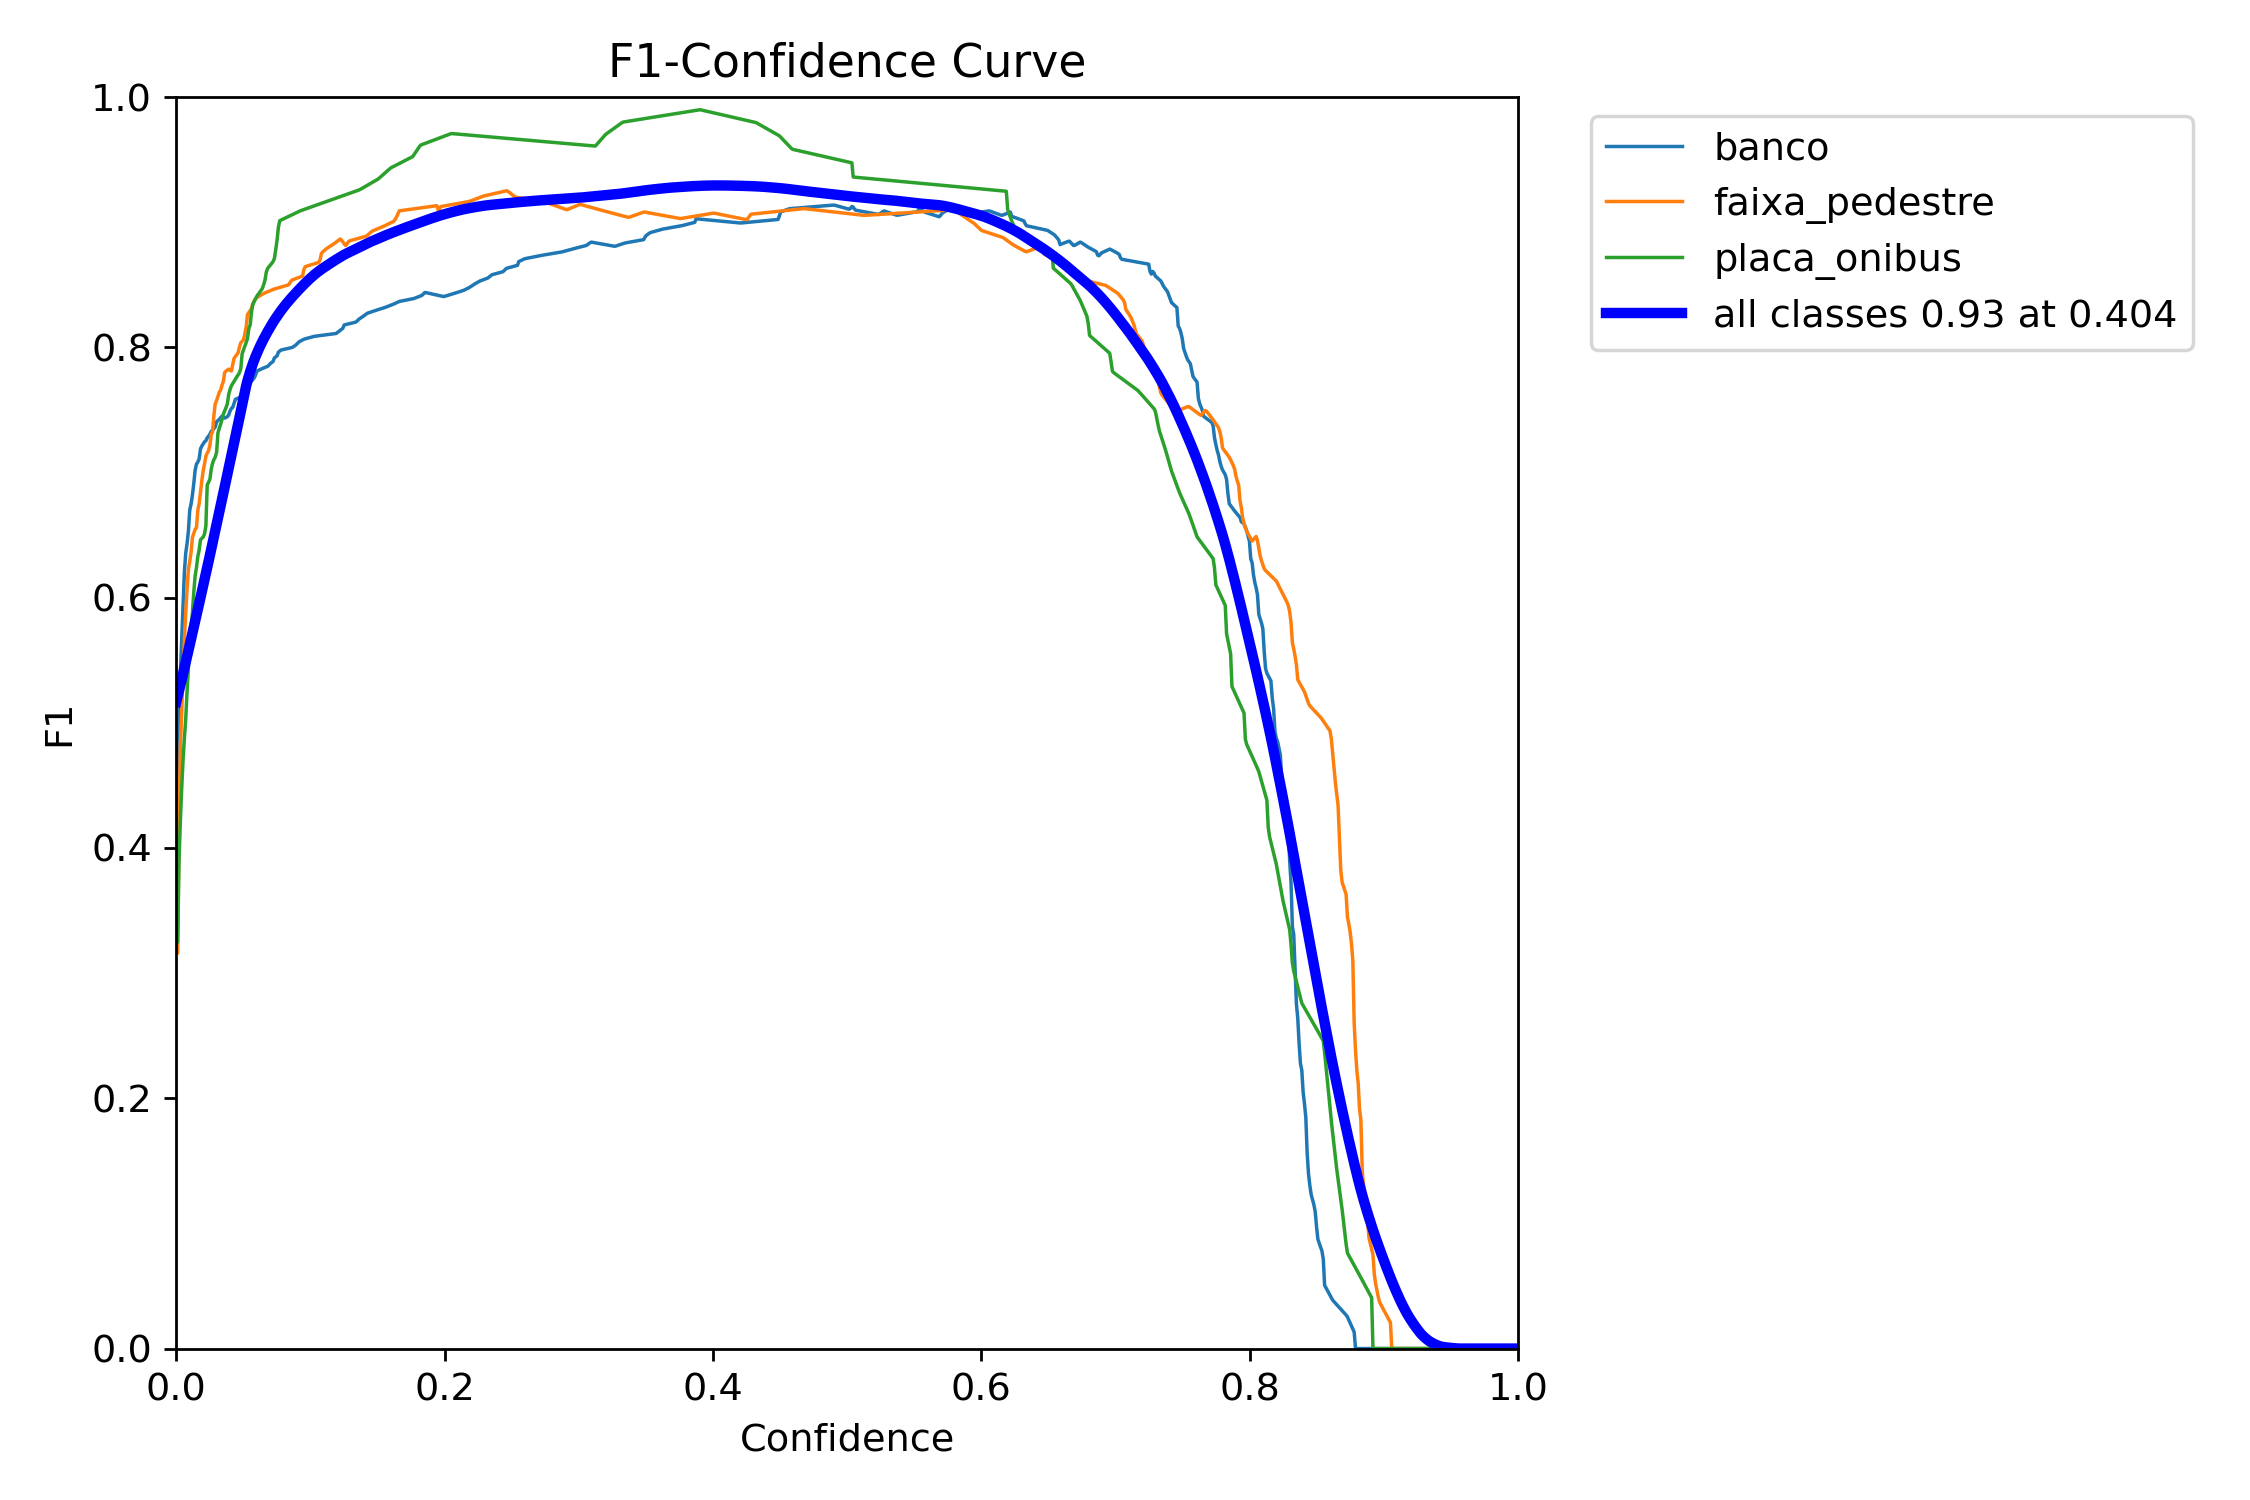
\includegraphics[width=1\textwidth]{Figuras/F1_curve.png}
  \\
  Fonte: Autoral.
  \label{fg-f1_curve}
\end{figure}
% --- Figura

Analisando individualmente as curvas de \textit{F1-Score} por classe, percebe-se que placa\_onibus mantém seu desempenho robusto mesmo em limiares mais altos, refletindo sua maior facilidade de detecção. Já as curvas de banco e faixa\_pedestre apresentam maiores variações, com picos de desempenho entre 0.35 e 0.55 de confiança, o que pode orientar o ajuste fino desses valores na aplicação prática.

Em termos de aplicação, especialmente em contextos assistivos, um maior \textit{recall} pode ser preferível, mesmo ao custo de alguns falsos positivos, desde que não comprometa a confiança do usuário no sistema. Assim, as curvas apresentadas servem não apenas como indicadores de desempenho, mas também como ferramentas de calibração para o uso prático do modelo.

\section{\textbf{Análise Qualitativa das Detecções em Cenários do Campus UFMG}}

Para além dos indicadores quantitativos, a análise qualitativa das detecções é fundamental para compreender a atuação prática do modelo em ambientes reais. Essa abordagem permite observar a qualidade visual das caixas delimitadoras, a confiabilidade das detecções em condições variadas e identificar situações específicas em que ocorrem erros, como falsos positivos ou falsos negativos, que podem não ser plenamente capturados pelas métricas agregadas.

A Figura \ref{fg-exemplo-deteccao-dia} apresenta um exemplo de detecção bem-sucedida, capturado durante o dia em local iluminado do campus Pampulha da UFMG. É possível observar múltiplas instâncias das classes de interesse sendo detectadas corretamente e com altos níveis de confiança (superiores a 0.80). As caixas delimitadoras são visualmente adequadas, envolvendo os objetos de forma precisa, com margens equilibradas e sem sobreposição excessiva com o fundo. Este resultado evidencia a capacidade do modelo em reconhecer simultaneamente diferentes objetos com confiabilidade, mesmo em ambientes dinâmicos, e reforça os elevados valores de \textit{precision} e mAP obtidos nas análises anteriores.

% --- Figura
\begin{figure}[htbp]
  \centering
  \caption{Exemplo de detecções corretas e bem localizadas para as classes banco e faixa\_pedestre em um cenário diurno no campus UFMG.}
  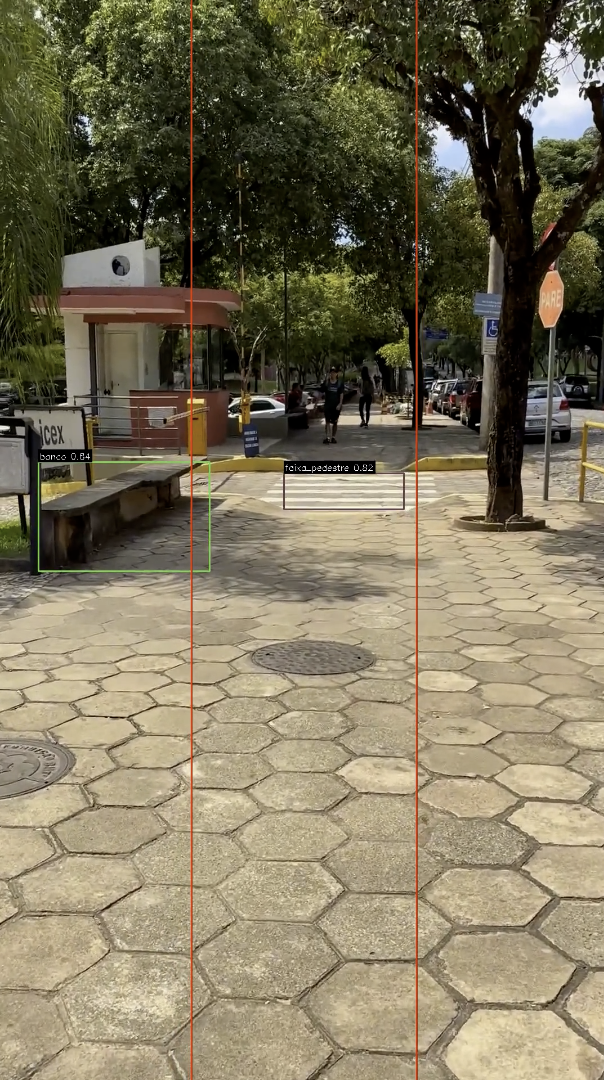
\includegraphics[width=0.6\textwidth]{Figuras/exemplo-deteccao-dia.png}
  \\
  Fonte: Autoral.
  \label{fg-exemplo-deteccao-dia}
\end{figure}
% --- Figura

Em contrapartida, a Figura \ref{fg-baixa_luminosidade} ilustra a atuação do modelo em uma situação de maior complexidade, com baixa iluminação ambiente. Nesse cenário, embora algumas detecções ainda sejam realizadas corretamente — como a identificação de uma placa\_onibus e dois bancos — observou-se uma leve redução na confiança das predições e uma maior variação na \textit{precision} espacial das caixas. Esse comportamento é esperado, dado que condições adversas de iluminação, especialmente à noite, impõem desafios à visão computacional, reduzindo o contraste e a nitidez dos objetos. Apesar disso, o modelo demonstrou capacidade de operar de forma aceitável mesmo sob essas limitações, o que reforça sua aplicabilidade em ambientes reais.

% --- Figura
\begin{figure}[htbp]
  \centering
  \caption{Desempenho do modelo em detecção de objetos sob condições de baixa luminosidade.}
  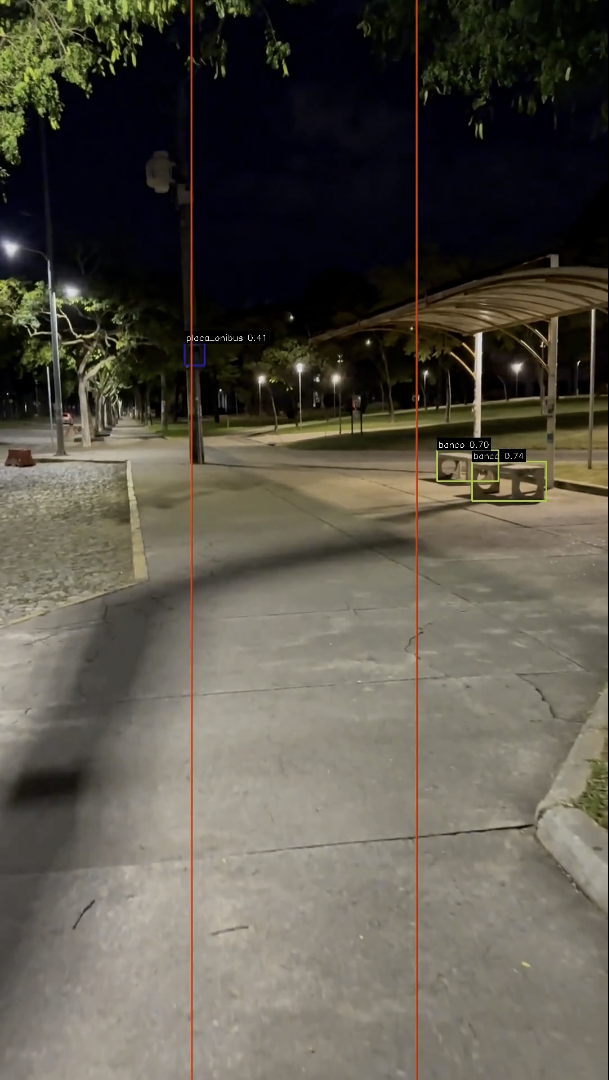
\includegraphics[width=0.6\textwidth]{Figuras/baixa_luminosidade.png}
  \\
  Fonte: Autoral.
  \label{fg-baixa_luminosidade}
\end{figure}
% --- Figura

A Figura 4.9 destaca um caso de falso positivo relacionado à classe faixa de pedestre. A imagem mostra uma região com elementos visuais semelhantes à aparência de uma faixa de pedestre (como listras brancas em cima de cada degrau), que foram incorretamente detectados como tal. Este tipo de equívoco pode ser reduzido no futuro com a inclusão de exemplos negativos mais específicos durante o treinamento ou pela aplicação de ajustes no limiar de confiança da inferência para essa classe.

% --- Figura
\begin{figure}[htbp]
  \centering
  \caption{Exemplo de um Falso Positivo para a classe 'faixa\_pedestre', onde o modelo detectou um objeto incorretamente.}
  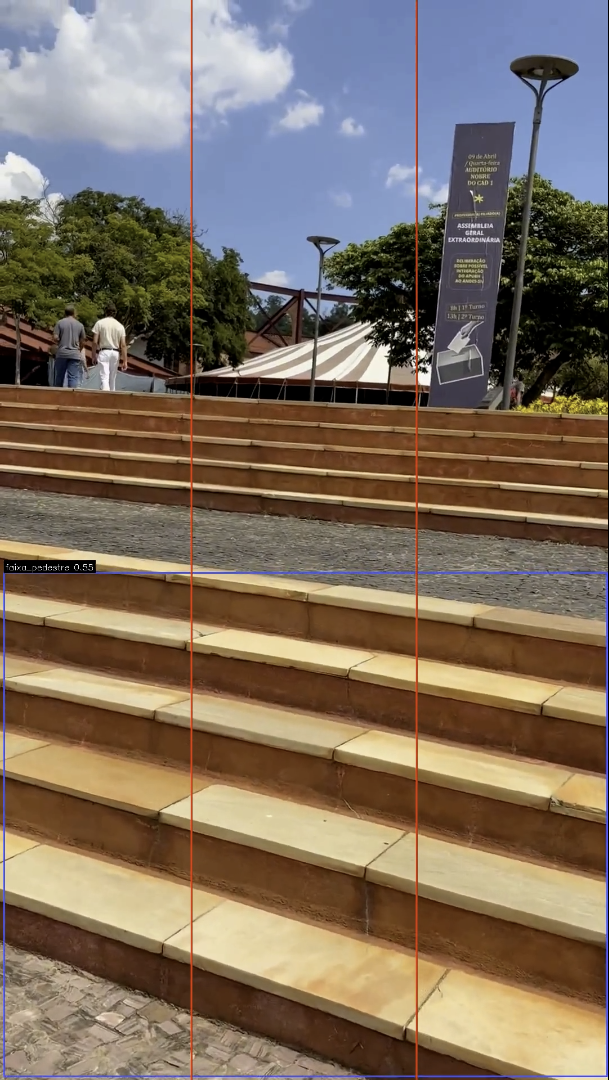
\includegraphics[width=0.6\textwidth]{Figuras/falso_positivo.png}
  \\
  Fonte: Autoral.
  \label{fg-falso_positivo}
\end{figure}
% --- Figura

Na Figura \ref{fg-falso_negativo}, evidencia-se um caso de falso negativo, em que uma faixa\_pedestre claramente visível não foi detectada pelo modelo. A provável causa está associada à condição de baixa iluminação e à presença de sombras que encobrem parcialmente o objeto. Tais situações ressaltam a importância da diversidade do \textit{dataset} e da inclusão de exemplos mais desafiadores, especialmente para objetos que sofrem alterações visuais relevantes em função do tempo ou das condições ambientais.

% --- Figura
\begin{figure}[htbp]
  \centering
  \caption{Exemplo de um Falso Negativo, onde o modelo não detectou um objeto presente.}
  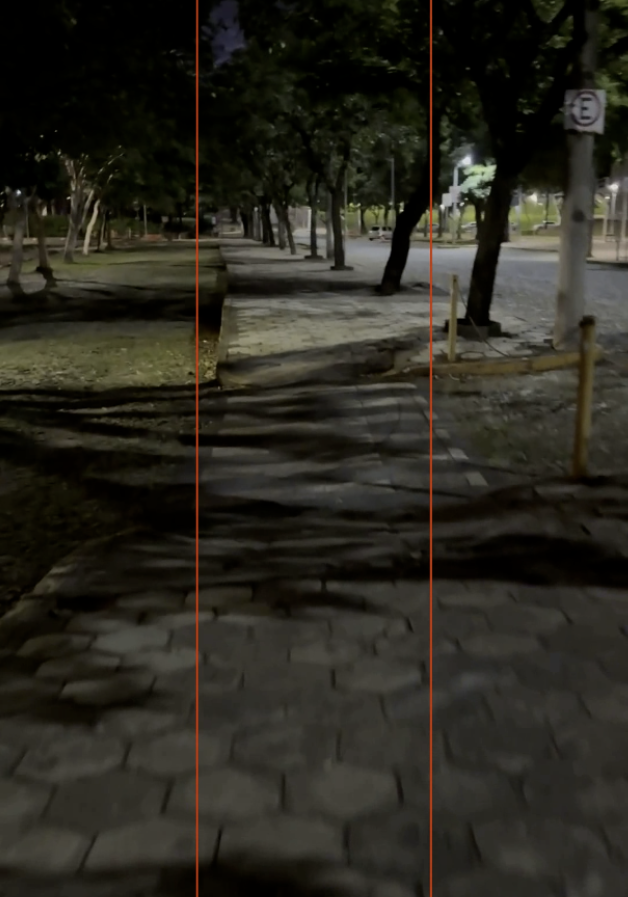
\includegraphics[width=0.6\textwidth]{Figuras/falso_negativo.png}
  \\
  Fonte: Autoral.
  \label{fg-falso_negativo}
\end{figure}
% --- Figura

Conclui-se, com base nesta análise qualitativa, que o modelo é robusto para a maioria dos cenários de uso previstos, mas que ainda existem oportunidades de melhoria, especialmente na redução de falsos positivos da classe banco e faixa de pedestre e no aumento da sensibilidade do modelo em situações de iluminação comprometida. Essas observações visuais corroboram os achados estatísticos apresentados nos tópicos anteriores e oferecem subsídios práticos para ajustes na implementação final do sistema assistivo.

\section{\textbf{Discussão Consolidada dos Resultados e Implicações para a Ferramenta Assistiva}}

A consolidação das análises quantitativa e qualitativa permite uma avaliação abrangente do modelo no que diz respeito à sua viabilidade como núcleo de uma ferramenta assistiva para pessoas com deficiência visual no campus da UFMG. Os resultados obtidos ao longo das avaliações apontam para um desempenho consistente, com alto potencial de aplicação prática e algumas limitações pontuais que podem ser endereçadas em fases posteriores do projeto.

O treinamento do modelo mostrou-se eficaz, com as curvas de perda e de mAP indicando um processo de aprendizagem estável, sem indícios de \textit{overfitting}. As métricas consolidadas no conjunto de validação, como o mAP@0.5 de 0.944 e o mAP@0.5:0.95 de 0.672, colocam o modelo em um patamar competitivo para aplicações reais, especialmente considerando que foi treinado com um volume relativamente modesto de dados. O uso da arquitetura YOLOv11, aliada a um \textit{dataset} bem curado e técnicas de \textit{data augmentation}, demonstrou ser uma escolha acertada, capaz de equilibrar velocidade de inferência e precisão.

No plano das métricas individuais, o desempenho foi particularmente elevado para a classe placa\_onibus, com valores próximos à perfeição em \textit{precision} e \textit{recall}. As classes faixa\_pedestre e banco também apresentaram bons resultados, ainda que a última tenha exibido maior propensão a falsos positivos. Isso indica que, embora o modelo tenha aprendido bem a distinguir visualmente as classes, algumas ambiguidades visuais ainda geram confusões com o fundo. Esse ponto poderá ser refinado com novos ciclos de treinamento, ajustes no limiar de confiança ou por meio de técnicas mais avançadas de regularização.

A análise das curvas de \textit{precision}-\textit{recall} e de \textit{F1-Score} reforçou a qualidade do modelo e ainda ofereceu um subsídio valioso para calibragem prática do sistema: a escolha de um limiar de confiança em torno de 0.4-0.5 tende a maximizar o equilíbrio entre acertos e erros. Essa configuração é especialmente relevante em aplicações assistivas, onde o excesso de alertas incorretos pode gerar desconfiança, e a omissão de objetos críticos pode comprometer a segurança do usuário. Assim, essa análise estatística apoia diretamente as decisões de projeto na integração da detecção com o sistema de \textit{background} auditivo.

As observações visuais das detecções, por sua vez, confirmam que o modelo é funcional em diversos cenários do campus, inclusive em horários noturnos e em ambientes parcialmente oclusos. Ainda que haja margem para melhorias, os resultados indicam que a ferramenta assistiva baseada nesse modelo tem potencial real para contribuir com a autonomia e a mobilidade de pessoas com deficiência visual. A velocidade de inferência, próxima de 20 a 30ms por imagem em ambiente de GPU, sugere viabilidade inclusive para aplicações futuras em tempo real, desde que se utilize \textit{hardware} com capacidade compatível.

Em síntese, o modelo desenvolvido atende de forma satisfatória aos objetivos propostos neste trabalho. Suas limitações são específicas, bem compreendidas e tecnicamente solucionáveis. A base técnica construída ao longo do projeto estabelece um ponto de partida sólido para a evolução da ferramenta, seja por meio de refinamento contínuo do modelo, integração com sensores complementares ou validação com usuários reais em ambientes de uso.
\chapter{\textbf{CONCLUSÃO}}

Este trabalho teve como objetivo desenvolver uma ferramenta baseada em inteligência artificial, utilizando o algoritmo YOLOv11, capaz de reconhecer objetos e elementos urbanos no campus Pampulha da UFMG, com o intuito de oferecer suporte à locomoção autônoma de pessoas com deficiência visual. A proposta buscou contribuir para a inclusão no ambiente universitário por meio do uso de tecnologias assistivas que possam promover maior autonomia e segurança.

Para atingir esse propósito, foi construída uma base de dados personalizada composta por imagens extraídas de vídeos gravados no próprio campus, considerando diferentes horários, condições de luminosidade e variações de ocupação dos espaços. As imagens foram anotadas manualmente e processadas utilizando técnicas de \textit{data augmentation}, com o objetivo de expandir a diversidade dos exemplos e garantir robustez ao modelo. O processo de treinamento foi realizado por meio do ambiente Google Colab, utilizando o modelo yolo11m.pt, com base em pesos pré-treinados e um conjunto de hiperparâmetros ajustado automaticamente pela biblioteca Ultralytics.

Os resultados quantitativos demonstraram que o modelo atingiu um desempenho robusto, com mAP@0.5 de 0.967 e mAP@0.5:0.95 de 0.670, o que indica boa capacidade tanto de classificação quanto de localização dos objetos de interesse. As métricas individuais por classe também se mostraram expressivas, especialmente para placa de ônibus e faixa de pedestre, com valores de \textit{precision} e \textit{recall} superiores a 0.970. A classe banco, embora com desempenho satisfatório, apresentou maior incidência de falsos positivos, sugerindo margem para aprimoramentos futuros no balanceamento do \textit{dataset} e na calibragem de limiares de confiança.

A análise qualitativa das detecções reforçou a eficácia prática do sistema, evidenciando sua capacidade de operar em diferentes cenários visuais, mesmo sob variações de iluminação. As limitações identificadas, como a maior confusão entre bancos e o \textit{background} em certas condições, bem como a ausência de testes com usuários reais e o funcionamento apenas com vídeos gravados (não em tempo real), não comprometem a viabilidade do projeto, mas delimitam seu escopo como uma prova de conceito funcional.

Embora não tenha sido possível implementar a aplicação em tempo real dentro do escopo deste trabalho, os resultados obtidos apontam para o potencial de aplicação futura dessa tecnologia em dispositivos móveis com \textit{background} auditivo automatizado. A ferramenta desenvolvida mostra-se promissora para auxiliar pessoas com deficiência visual na navegação em ambientes públicos complexos como o campus universitário, contribuindo com os princípios de acessibilidade e inclusão.

Como sugestões para trabalhos futuros, destaca-se a possibilidade de expandir o número de classes de objetos detectados, realizar testes em tempo real com câmeras acopladas a dispositivos móveis, integrar a ferramenta com sistemas de \textit{background} por vibração ou áudio adaptativo, e sobretudo, conduzir testes com usuários reais, o que poderá fornecer insights mais profundos sobre a usabilidade, eficiência e impacto social da ferramenta proposta.

Dessa forma, este trabalho não apenas cumpre seus objetivos iniciais, como estabelece uma base sólida para o desenvolvimento contínuo de soluções tecnológicas voltadas à acessibilidade, aliando inovação técnica e compromisso com a inclusão social no espaço universitário.
\clearpage
\small
%%%%%%%%%%%%%%%%%%%%%%%%%%%%%%%%%%%%%%%%%%%%%%%%
\bibliographystyle{abntex2-alf}
\bibliography{bibliografia}
\label{ultima_pagina}
%---------------------
\end{document}
